% **************************************************************************************************************
% A Classic Thesis Style
% An Homage to The Elements of Typographic Style
%
% Copyright (C) 2017 André Miede and Ivo Pletikosić
%
% If you like the style then I would appreciate a postcard. My address
% can be found in the file ClassicThesis.pdf. A collection of the
% postcards I received so far is available online at
% http://postcards.miede.de
%
% License:
% This program is free software; you can redistribute it and/or modify
% it under the terms of the GNU General Public License as published by
% the Free Software Foundation; either version 2 of the License, or
% (at your option) any later version.
%
% This program is distributed in the hope that it will be useful,
% but WITHOUT ANY WARRANTY; without even the implied warranty of
% MERCHANTABILITY or FITNESS FOR A PARTICULAR PURPOSE.  See the
% GNU General Public License for more details.
%
% You should have received a copy of the GNU General Public License
% along with this program; see the file COPYING.  If not, write to
% the Free Software Foundation, Inc., 59 Temple Place - Suite 330,
% Boston, MA 02111-1307, USA.
%
% PLEASE SEE ALSO THE AUTHORS' NOTE REGARDING THIS LICENSE
% IN THE DOCUMENTATION (ClassicThesis.pdf --> Chapter 1 / Chapter01.tex)
% **************************************************************************************************************
\RequirePackage{silence} % :-\
    \WarningFilter{scrreprt}{Usage of package `titlesec'}
    %\WarningFilter{scrreprt}{Activating an ugly workaround}
    \WarningFilter{titlesec}{Non standard sectioning command detected}
\documentclass[ oneside,openright,titlepage,numbers=noenddot,headinclude,%1headlines,% letterpaper a4paper
                footinclude=true,cleardoublepage=empty,abstractoff, % <--- obsolete, remove (todo)
                BCOR=5mm,paper=a4,fontsize=11pt,%11pt,a4paper,%
                ngerman,american,italian%
                ]{scrreprt}

%********************************************************************
% Note: Make all your adjustments in here
%*******************************************************
% ****************************************************************************************************
% classicthesis-config.tex
% formerly known as loadpackages.sty, classicthesis-ldpkg.sty, and classicthesis-preamble.sty
% Use it at the beginning of your ClassicThesis.tex, or as a LaTeX Preamble
% in your ClassicThesis.{tex,lyx} with % ****************************************************************************************************
% classicthesis-config.tex
% formerly known as loadpackages.sty, classicthesis-ldpkg.sty, and classicthesis-preamble.sty
% Use it at the beginning of your ClassicThesis.tex, or as a LaTeX Preamble
% in your ClassicThesis.{tex,lyx} with % ****************************************************************************************************
% classicthesis-config.tex
% formerly known as loadpackages.sty, classicthesis-ldpkg.sty, and classicthesis-preamble.sty
% Use it at the beginning of your ClassicThesis.tex, or as a LaTeX Preamble
% in your ClassicThesis.{tex,lyx} with \input{classicthesis-config}
% ****************************************************************************************************
% If you like the classicthesis, then I would appreciate a postcard.
% My address can be found in the file ClassicThesis.pdf. A collection
% of the postcards I received so far is available online at
% http://postcards.miede.de
% ****************************************************************************************************


% ****************************************************************************************************
% 0. Set the encoding of your files. UTF-8 is the only sensible encoding nowadays. If you can't read
% äöüßáéçèê∂åëæƒÏ€ then change the encoding setting in your editor, not the line below. If your editor
% does not support utf8 use another editor!
% ****************************************************************************************************
\PassOptionsToPackage{utf8}{inputenc}
  \usepackage{inputenc}

% ****************************************************************************************************
% 1. Configure classicthesis for your needs here, e.g., remove "drafting" below
% in order to deactivate the time-stamp on the pages
% (see ClassicThesis.pdf for more information):
% ****************************************************************************************************
\PassOptionsToPackage{
  drafting=false,    % print version information on the bottom of the pages
  tocaligned=false, % the left column of the toc will be aligned (no indentation)
  dottedtoc=false,  % page numbers in ToC flushed right
  parts=true,       % use part division
  eulerchapternumbers=true, % use AMS Euler for chapter font (otherwise Palatino)
  linedheaders=false,       % chaper headers will have line above and beneath
  floatperchapter=true,     % numbering per chapter for all floats (i.e., Figure 1.1)
  eulermath=true,  % use awesome Euler fonts for mathematical formulae (only with pdfLaTeX)
  beramono=true,    % toggle a nice monospaced font (w/ bold)
  % palatino=false,   % deactivate standard font for loading another one, see the last section at the end of this file for suggestions
}{classicthesis}


% ****************************************************************************************************
% 2. Personal data and user ad-hoc commands
% ****************************************************************************************************
\newcommand{\myTitle}{Design of Real-Time Optical Coherence Tomography\xspace}
\newcommand{\mySubtitle}{Master Thesis in Telecommunication Engineering\xspace}
%\newcommand{\myDegree}{Doktor-Ingenieur (Dr.-Ing.)\xspace}
\newcommand{\myName}{Gianluca Marcon\xspace}
\newcommand{\myProf}{Luca Palmieri\xspace}
%\newcommand{\myOtherProf}{Put name here\xspace}
%\newcommand{\mySupervisor}{Put name here\xspace}
\newcommand{\myFaculty}{Put data here\xspace}
\newcommand{\myDepartment}{Department of Information Engineering\xspace}
\newcommand{\myUni}{Università degli Studi di Padova\xspace}
\newcommand{\myLocation}{Saarbrücken\xspace}
\newcommand{\myTime}{April 2018\xspace}
\newcommand{\myVersion}{version 1.0}

% ********************************************************************
% Setup, finetuning, and useful commands
% ********************************************************************
\newcounter{dummy} % necessary for correct hyperlinks (to index, bib, etc.)
\newlength{\abcd} % for ab..z string length calculation
\providecommand{\mLyX}{L\kern-.1667em\lower.25em\hbox{Y}\kern-.125emX\@}
\newcommand{\ie}{i.\,e.}
\newcommand{\Ie}{I.\,e.}
\newcommand{\eg}{e.\,g.}
\newcommand{\Eg}{E.\,g.}
% ****************************************************************************************************


% ****************************************************************************************************
% 3. Loading some handy packages
% ****************************************************************************************************
% ********************************************************************
% Packages with options that might require adjustments
% ********************************************************************
\PassOptionsToPackage{italian,american}{babel} % change this to your language(s), main language last
% Spanish languages need extra options in order to work with this template
%\PassOptionsToPackage{spanish,es-lcroman}{babel}
    \usepackage{babel}

\usepackage{csquotes}
\PassOptionsToPackage{%
  %backend=biber,bibencoding=utf8, %instead of bibtex
  backend=bibtex8,bibencoding=ascii,%
  language=auto,%
  style=numeric-comp,%
  %style=authoryear-comp, % Author 1999, 2010
  %bibstyle=authoryear,dashed=false, % dashed: substitute rep. author with ---
  sorting=nyt, % name, year, title
  maxbibnames=10, % default: 3, et al.
  %backref=true,%
  natbib=true % natbib compatibility mode (\citep and \citet still work)
}{biblatex}
    \usepackage{biblatex}

\PassOptionsToPackage{fleqn}{amsmath}       % math environments and more by the AMS
  \usepackage{amsmath}

% ********************************************************************
% General useful packages
% ********************************************************************
\PassOptionsToPackage{T1}{fontenc} % T2A for cyrillics
  \usepackage{fontenc}
\usepackage{textcomp} % fix warning with missing font shapes
\usepackage{scrhack} % fix warnings when using KOMA with listings package
\usepackage{xspace} % to get the spacing after macros right
\usepackage{mparhack} % get marginpar right
%\usepackage{fixltx2e} % fixes some LaTeX stuff --> since 2015 in the LaTeX kernel (see below)
% \usepackage[latest]{latexrelease} % emulate newer kernel version if older is detected
\PassOptionsToPackage{printonlyused,smaller}{acronym}
  \usepackage{acronym} % nice macros for handling all acronyms in the thesis
  %\renewcommand{\bflabel}[1]{{#1}\hfill} % fix the list of acronyms --> no longer working
  %\renewcommand*{\acsfont}[1]{\textsc{#1}}
  %\renewcommand*{\aclabelfont}[1]{\acsfont{#1}}
  %\def\bflabel#1{{#1\hfill}}
  \def\bflabel#1{{\acsfont{#1}\hfill}}
  \def\aclabelfont#1{\acsfont{#1}}
% ****************************************************************************************************
%\usepackage{pgfplots} % External TikZ/PGF support (thanks to Andreas Nautsch)
%\usetikzlibrary{external}
%\tikzexternalize[mode=list and make, prefix=ext-tikz/]
% ****************************************************************************************************


% ****************************************************************************************************
% 4. Setup floats: tables, (sub)figures, and captions
% ****************************************************************************************************
\usepackage{tabularx} % better tables
  \setlength{\extrarowheight}{3pt} % increase table row height
\newcommand{\tableheadline}[1]{\multicolumn{1}{l}{\spacedlowsmallcaps{#1}}}
\newcommand{\myfloatalign}{\centering} % to be used with each float for alignment
\usepackage{caption}
% Thanks to cgnieder and Claus Lahiri
% http://tex.stackexchange.com/questions/69349/spacedlowsmallcaps-in-caption-label
% [REMOVED DUE TO OTHER PROBLEMS, SEE ISSUE #82]
%\DeclareCaptionLabelFormat{smallcaps}{\bothIfFirst{#1}{~}\MakeTextLowercase{\textsc{#2}}}
%\captionsetup{font=small,labelformat=smallcaps} % format=hang,
\captionsetup{font=small} % format=hang,
\usepackage{subfig}
% ****************************************************************************************************


% ****************************************************************************************************
% 5. Setup code listings
% ****************************************************************************************************
\usepackage{listings}
%\lstset{emph={trueIndex,root},emphstyle=\color{BlueViolet}}%\underbar} % for special keywords
\lstset{language=[LaTeX]Tex,%C++,
  morekeywords={PassOptionsToPackage,selectlanguage},
  keywordstyle=\color{RoyalBlue},%\bfseries,
  basicstyle=\small\ttfamily,
  %identifierstyle=\color{NavyBlue},
  commentstyle=\color{Green}\ttfamily,
  stringstyle=\rmfamily,
  numbers=none,%left,%
  numberstyle=\scriptsize,%\tiny
  stepnumber=5,
  numbersep=8pt,
  showstringspaces=false,
  breaklines=true,
  %frameround=ftff,
  %frame=single,
  belowcaptionskip=.75\baselineskip
  %frame=L
}
% ****************************************************************************************************


% ****************************************************************************************************
% 6. PDFLaTeX, hyperreferences, and citation backreferences
% ****************************************************************************************************
% ********************************************************************
% Using PDFLaTeX
% ********************************************************************
\PassOptionsToPackage{hyperfootnotes=false,pdfpagelabels}{hyperref}
  \usepackage{hyperref}  % backref linktocpage pagebackref
  \usepackage{graphicx}


% ********************************************************************
% Hyperreferences
% ********************************************************************
\hypersetup{%
  %draft, % hyperref's draft mode, for printing see below
  colorlinks=true, linktocpage=true, pdfstartpage=3, pdfstartview=FitV,%
  % uncomment the following line if you want to have black links (e.g., for printing)
  %colorlinks=false, linktocpage=false, pdfstartpage=3, pdfstartview=FitV, pdfborder={0 0 0},%
  breaklinks=true, pdfpagemode=UseNone, pageanchor=true, pdfpagemode=UseOutlines,%
  plainpages=false, bookmarksnumbered, bookmarksopen=true, bookmarksopenlevel=1,%
  hypertexnames=true, pdfhighlight=/O,%nesting=true,%frenchlinks,%
  urlcolor=webbrown, linkcolor=RoyalBlue, citecolor=webgreen, %pagecolor=RoyalBlue,%
  %urlcolor=Black, linkcolor=Black, citecolor=Black, %pagecolor=Black,%
  pdftitle={\myTitle},%
  pdfauthor={\textcopyright\ \myName, \myUni, \myFaculty},%
  pdfsubject={},%
  pdfkeywords={},%
  pdfcreator={pdfLaTeX},%
  pdfproducer={LaTeX with hyperref and classicthesis}%
}

% ********************************************************************
% Setup autoreferences
% ********************************************************************
% There are some issues regarding autorefnames
% http://www.ureader.de/msg/136221647.aspx
% http://www.tex.ac.uk/cgi-bin/texfaq2html?label=latexwords
% you have to redefine the makros for the
% language you use, e.g., american, ngerman
% (as chosen when loading babel/AtBeginDocument)
% ********************************************************************
\makeatletter
\@ifpackageloaded{babel}%
  {%
    \addto\extrasamerican{%
      \renewcommand*{\figureautorefname}{Figure}%
      \renewcommand*{\tableautorefname}{Table}%
      \renewcommand*{\partautorefname}{Part}%
      \renewcommand*{\chapterautorefname}{Chapter}%
      \renewcommand*{\sectionautorefname}{Section}%
      \renewcommand*{\subsectionautorefname}{Section}%
      \renewcommand*{\subsubsectionautorefname}{Section}%
    }%
    \addto\extrasngerman{%
      \renewcommand*{\paragraphautorefname}{Absatz}%
      \renewcommand*{\subparagraphautorefname}{Unterabsatz}%
      \renewcommand*{\footnoteautorefname}{Fu\"snote}%
      \renewcommand*{\FancyVerbLineautorefname}{Zeile}%
      \renewcommand*{\theoremautorefname}{Theorem}%
      \renewcommand*{\appendixautorefname}{Anhang}%
      \renewcommand*{\equationautorefname}{Gleichung}%
      \renewcommand*{\itemautorefname}{Punkt}%
    }%
      % Fix to getting autorefs for subfigures right (thanks to Belinda Vogt for changing the definition)
      \providecommand{\subfigureautorefname}{\figureautorefname}%
    }{\relax}
\makeatother


% ****************************************************************************************************
% 7. Last calls before the bar closes
% ****************************************************************************************************
% ********************************************************************
% Development Stuff
% ********************************************************************
\listfiles
%\PassOptionsToPackage{l2tabu,orthodox,abort}{nag}
%  \usepackage{nag}
%\PassOptionsToPackage{warning, all}{onlyamsmath}
%  \usepackage{onlyamsmath}

% ********************************************************************
% Last, but not least...
% ********************************************************************
\usepackage{classicthesis}
% ****************************************************************************************************


% ****************************************************************************************************
% 8. Further adjustments (experimental)
% ****************************************************************************************************
% ********************************************************************
% Changing the text area
% ********************************************************************
%\areaset[current]{312pt}{761pt} % 686 (factor 2.2) + 33 head + 42 head \the\footskip
%\setlength{\marginparwidth}{7em}%
%\setlength{\marginparsep}{2em}%

% ********************************************************************
% Using different fonts
% ********************************************************************
%\usepackage[oldstylenums]{kpfonts} % oldstyle notextcomp
% \usepackage[osf]{libertine}
%\usepackage[light,condensed,math]{iwona}
%\renewcommand{\sfdefault}{iwona}
%\usepackage{lmodern} % <-- no osf support :-(
%\usepackage{cfr-lm} %
%\usepackage[urw-garamond]{mathdesign} <-- no osf support :-(
%\usepackage[default,osfigures]{opensans} % scale=0.95
%\usepackage[sfdefault]{FiraSans}
% \usepackage[opticals,mathlf]{MinionPro} % onlytext
% ********************************************************************
%\usepackage[largesc,osf]{newpxtext}
%\linespread{1.05} % a bit more for Palatino
% Used to fix these:
% https://bitbucket.org/amiede/classicthesis/issues/139/italics-in-pallatino-capitals-chapter
% https://bitbucket.org/amiede/classicthesis/issues/45/problema-testatine-su-classicthesis-style
% ********************************************************************
% ****************************************************************************************************

% ****************************************************************************************************
% If you like the classicthesis, then I would appreciate a postcard.
% My address can be found in the file ClassicThesis.pdf. A collection
% of the postcards I received so far is available online at
% http://postcards.miede.de
% ****************************************************************************************************


% ****************************************************************************************************
% 0. Set the encoding of your files. UTF-8 is the only sensible encoding nowadays. If you can't read
% äöüßáéçèê∂åëæƒÏ€ then change the encoding setting in your editor, not the line below. If your editor
% does not support utf8 use another editor!
% ****************************************************************************************************
\PassOptionsToPackage{utf8}{inputenc}
  \usepackage{inputenc}

% ****************************************************************************************************
% 1. Configure classicthesis for your needs here, e.g., remove "drafting" below
% in order to deactivate the time-stamp on the pages
% (see ClassicThesis.pdf for more information):
% ****************************************************************************************************
\PassOptionsToPackage{
  drafting=false,    % print version information on the bottom of the pages
  tocaligned=false, % the left column of the toc will be aligned (no indentation)
  dottedtoc=false,  % page numbers in ToC flushed right
  parts=true,       % use part division
  eulerchapternumbers=true, % use AMS Euler for chapter font (otherwise Palatino)
  linedheaders=false,       % chaper headers will have line above and beneath
  floatperchapter=true,     % numbering per chapter for all floats (i.e., Figure 1.1)
  eulermath=true,  % use awesome Euler fonts for mathematical formulae (only with pdfLaTeX)
  beramono=true,    % toggle a nice monospaced font (w/ bold)
  % palatino=false,   % deactivate standard font for loading another one, see the last section at the end of this file for suggestions
}{classicthesis}


% ****************************************************************************************************
% 2. Personal data and user ad-hoc commands
% ****************************************************************************************************
\newcommand{\myTitle}{Design of Real-Time Optical Coherence Tomography\xspace}
\newcommand{\mySubtitle}{Master Thesis in Telecommunication Engineering\xspace}
%\newcommand{\myDegree}{Doktor-Ingenieur (Dr.-Ing.)\xspace}
\newcommand{\myName}{Gianluca Marcon\xspace}
\newcommand{\myProf}{Luca Palmieri\xspace}
%\newcommand{\myOtherProf}{Put name here\xspace}
%\newcommand{\mySupervisor}{Put name here\xspace}
\newcommand{\myFaculty}{Put data here\xspace}
\newcommand{\myDepartment}{Department of Information Engineering\xspace}
\newcommand{\myUni}{Università degli Studi di Padova\xspace}
\newcommand{\myLocation}{Saarbrücken\xspace}
\newcommand{\myTime}{April 2018\xspace}
\newcommand{\myVersion}{version 1.0}

% ********************************************************************
% Setup, finetuning, and useful commands
% ********************************************************************
\newcounter{dummy} % necessary for correct hyperlinks (to index, bib, etc.)
\newlength{\abcd} % for ab..z string length calculation
\providecommand{\mLyX}{L\kern-.1667em\lower.25em\hbox{Y}\kern-.125emX\@}
\newcommand{\ie}{i.\,e.}
\newcommand{\Ie}{I.\,e.}
\newcommand{\eg}{e.\,g.}
\newcommand{\Eg}{E.\,g.}
% ****************************************************************************************************


% ****************************************************************************************************
% 3. Loading some handy packages
% ****************************************************************************************************
% ********************************************************************
% Packages with options that might require adjustments
% ********************************************************************
\PassOptionsToPackage{italian,american}{babel} % change this to your language(s), main language last
% Spanish languages need extra options in order to work with this template
%\PassOptionsToPackage{spanish,es-lcroman}{babel}
    \usepackage{babel}

\usepackage{csquotes}
\PassOptionsToPackage{%
  %backend=biber,bibencoding=utf8, %instead of bibtex
  backend=bibtex8,bibencoding=ascii,%
  language=auto,%
  style=numeric-comp,%
  %style=authoryear-comp, % Author 1999, 2010
  %bibstyle=authoryear,dashed=false, % dashed: substitute rep. author with ---
  sorting=nyt, % name, year, title
  maxbibnames=10, % default: 3, et al.
  %backref=true,%
  natbib=true % natbib compatibility mode (\citep and \citet still work)
}{biblatex}
    \usepackage{biblatex}

\PassOptionsToPackage{fleqn}{amsmath}       % math environments and more by the AMS
  \usepackage{amsmath}

% ********************************************************************
% General useful packages
% ********************************************************************
\PassOptionsToPackage{T1}{fontenc} % T2A for cyrillics
  \usepackage{fontenc}
\usepackage{textcomp} % fix warning with missing font shapes
\usepackage{scrhack} % fix warnings when using KOMA with listings package
\usepackage{xspace} % to get the spacing after macros right
\usepackage{mparhack} % get marginpar right
%\usepackage{fixltx2e} % fixes some LaTeX stuff --> since 2015 in the LaTeX kernel (see below)
% \usepackage[latest]{latexrelease} % emulate newer kernel version if older is detected
\PassOptionsToPackage{printonlyused,smaller}{acronym}
  \usepackage{acronym} % nice macros for handling all acronyms in the thesis
  %\renewcommand{\bflabel}[1]{{#1}\hfill} % fix the list of acronyms --> no longer working
  %\renewcommand*{\acsfont}[1]{\textsc{#1}}
  %\renewcommand*{\aclabelfont}[1]{\acsfont{#1}}
  %\def\bflabel#1{{#1\hfill}}
  \def\bflabel#1{{\acsfont{#1}\hfill}}
  \def\aclabelfont#1{\acsfont{#1}}
% ****************************************************************************************************
%\usepackage{pgfplots} % External TikZ/PGF support (thanks to Andreas Nautsch)
%\usetikzlibrary{external}
%\tikzexternalize[mode=list and make, prefix=ext-tikz/]
% ****************************************************************************************************


% ****************************************************************************************************
% 4. Setup floats: tables, (sub)figures, and captions
% ****************************************************************************************************
\usepackage{tabularx} % better tables
  \setlength{\extrarowheight}{3pt} % increase table row height
\newcommand{\tableheadline}[1]{\multicolumn{1}{l}{\spacedlowsmallcaps{#1}}}
\newcommand{\myfloatalign}{\centering} % to be used with each float for alignment
\usepackage{caption}
% Thanks to cgnieder and Claus Lahiri
% http://tex.stackexchange.com/questions/69349/spacedlowsmallcaps-in-caption-label
% [REMOVED DUE TO OTHER PROBLEMS, SEE ISSUE #82]
%\DeclareCaptionLabelFormat{smallcaps}{\bothIfFirst{#1}{~}\MakeTextLowercase{\textsc{#2}}}
%\captionsetup{font=small,labelformat=smallcaps} % format=hang,
\captionsetup{font=small} % format=hang,
\usepackage{subfig}
% ****************************************************************************************************


% ****************************************************************************************************
% 5. Setup code listings
% ****************************************************************************************************
\usepackage{listings}
%\lstset{emph={trueIndex,root},emphstyle=\color{BlueViolet}}%\underbar} % for special keywords
\lstset{language=[LaTeX]Tex,%C++,
  morekeywords={PassOptionsToPackage,selectlanguage},
  keywordstyle=\color{RoyalBlue},%\bfseries,
  basicstyle=\small\ttfamily,
  %identifierstyle=\color{NavyBlue},
  commentstyle=\color{Green}\ttfamily,
  stringstyle=\rmfamily,
  numbers=none,%left,%
  numberstyle=\scriptsize,%\tiny
  stepnumber=5,
  numbersep=8pt,
  showstringspaces=false,
  breaklines=true,
  %frameround=ftff,
  %frame=single,
  belowcaptionskip=.75\baselineskip
  %frame=L
}
% ****************************************************************************************************


% ****************************************************************************************************
% 6. PDFLaTeX, hyperreferences, and citation backreferences
% ****************************************************************************************************
% ********************************************************************
% Using PDFLaTeX
% ********************************************************************
\PassOptionsToPackage{hyperfootnotes=false,pdfpagelabels}{hyperref}
  \usepackage{hyperref}  % backref linktocpage pagebackref
  \usepackage{graphicx}


% ********************************************************************
% Hyperreferences
% ********************************************************************
\hypersetup{%
  %draft, % hyperref's draft mode, for printing see below
  colorlinks=true, linktocpage=true, pdfstartpage=3, pdfstartview=FitV,%
  % uncomment the following line if you want to have black links (e.g., for printing)
  %colorlinks=false, linktocpage=false, pdfstartpage=3, pdfstartview=FitV, pdfborder={0 0 0},%
  breaklinks=true, pdfpagemode=UseNone, pageanchor=true, pdfpagemode=UseOutlines,%
  plainpages=false, bookmarksnumbered, bookmarksopen=true, bookmarksopenlevel=1,%
  hypertexnames=true, pdfhighlight=/O,%nesting=true,%frenchlinks,%
  urlcolor=webbrown, linkcolor=RoyalBlue, citecolor=webgreen, %pagecolor=RoyalBlue,%
  %urlcolor=Black, linkcolor=Black, citecolor=Black, %pagecolor=Black,%
  pdftitle={\myTitle},%
  pdfauthor={\textcopyright\ \myName, \myUni, \myFaculty},%
  pdfsubject={},%
  pdfkeywords={},%
  pdfcreator={pdfLaTeX},%
  pdfproducer={LaTeX with hyperref and classicthesis}%
}

% ********************************************************************
% Setup autoreferences
% ********************************************************************
% There are some issues regarding autorefnames
% http://www.ureader.de/msg/136221647.aspx
% http://www.tex.ac.uk/cgi-bin/texfaq2html?label=latexwords
% you have to redefine the makros for the
% language you use, e.g., american, ngerman
% (as chosen when loading babel/AtBeginDocument)
% ********************************************************************
\makeatletter
\@ifpackageloaded{babel}%
  {%
    \addto\extrasamerican{%
      \renewcommand*{\figureautorefname}{Figure}%
      \renewcommand*{\tableautorefname}{Table}%
      \renewcommand*{\partautorefname}{Part}%
      \renewcommand*{\chapterautorefname}{Chapter}%
      \renewcommand*{\sectionautorefname}{Section}%
      \renewcommand*{\subsectionautorefname}{Section}%
      \renewcommand*{\subsubsectionautorefname}{Section}%
    }%
    \addto\extrasngerman{%
      \renewcommand*{\paragraphautorefname}{Absatz}%
      \renewcommand*{\subparagraphautorefname}{Unterabsatz}%
      \renewcommand*{\footnoteautorefname}{Fu\"snote}%
      \renewcommand*{\FancyVerbLineautorefname}{Zeile}%
      \renewcommand*{\theoremautorefname}{Theorem}%
      \renewcommand*{\appendixautorefname}{Anhang}%
      \renewcommand*{\equationautorefname}{Gleichung}%
      \renewcommand*{\itemautorefname}{Punkt}%
    }%
      % Fix to getting autorefs for subfigures right (thanks to Belinda Vogt for changing the definition)
      \providecommand{\subfigureautorefname}{\figureautorefname}%
    }{\relax}
\makeatother


% ****************************************************************************************************
% 7. Last calls before the bar closes
% ****************************************************************************************************
% ********************************************************************
% Development Stuff
% ********************************************************************
\listfiles
%\PassOptionsToPackage{l2tabu,orthodox,abort}{nag}
%  \usepackage{nag}
%\PassOptionsToPackage{warning, all}{onlyamsmath}
%  \usepackage{onlyamsmath}

% ********************************************************************
% Last, but not least...
% ********************************************************************
\usepackage{classicthesis}
% ****************************************************************************************************


% ****************************************************************************************************
% 8. Further adjustments (experimental)
% ****************************************************************************************************
% ********************************************************************
% Changing the text area
% ********************************************************************
%\areaset[current]{312pt}{761pt} % 686 (factor 2.2) + 33 head + 42 head \the\footskip
%\setlength{\marginparwidth}{7em}%
%\setlength{\marginparsep}{2em}%

% ********************************************************************
% Using different fonts
% ********************************************************************
%\usepackage[oldstylenums]{kpfonts} % oldstyle notextcomp
% \usepackage[osf]{libertine}
%\usepackage[light,condensed,math]{iwona}
%\renewcommand{\sfdefault}{iwona}
%\usepackage{lmodern} % <-- no osf support :-(
%\usepackage{cfr-lm} %
%\usepackage[urw-garamond]{mathdesign} <-- no osf support :-(
%\usepackage[default,osfigures]{opensans} % scale=0.95
%\usepackage[sfdefault]{FiraSans}
% \usepackage[opticals,mathlf]{MinionPro} % onlytext
% ********************************************************************
%\usepackage[largesc,osf]{newpxtext}
%\linespread{1.05} % a bit more for Palatino
% Used to fix these:
% https://bitbucket.org/amiede/classicthesis/issues/139/italics-in-pallatino-capitals-chapter
% https://bitbucket.org/amiede/classicthesis/issues/45/problema-testatine-su-classicthesis-style
% ********************************************************************
% ****************************************************************************************************

% ****************************************************************************************************
% If you like the classicthesis, then I would appreciate a postcard.
% My address can be found in the file ClassicThesis.pdf. A collection
% of the postcards I received so far is available online at
% http://postcards.miede.de
% ****************************************************************************************************


% ****************************************************************************************************
% 0. Set the encoding of your files. UTF-8 is the only sensible encoding nowadays. If you can't read
% äöüßáéçèê∂åëæƒÏ€ then change the encoding setting in your editor, not the line below. If your editor
% does not support utf8 use another editor!
% ****************************************************************************************************
\PassOptionsToPackage{utf8}{inputenc}
  \usepackage{inputenc}

% ****************************************************************************************************
% 1. Configure classicthesis for your needs here, e.g., remove "drafting" below
% in order to deactivate the time-stamp on the pages
% (see ClassicThesis.pdf for more information):
% ****************************************************************************************************
\PassOptionsToPackage{
  drafting=false,    % print version information on the bottom of the pages
  tocaligned=false, % the left column of the toc will be aligned (no indentation)
  dottedtoc=false,  % page numbers in ToC flushed right
  parts=true,       % use part division
  eulerchapternumbers=true, % use AMS Euler for chapter font (otherwise Palatino)
  linedheaders=false,       % chaper headers will have line above and beneath
  floatperchapter=true,     % numbering per chapter for all floats (i.e., Figure 1.1)
  eulermath=true,  % use awesome Euler fonts for mathematical formulae (only with pdfLaTeX)
  beramono=true,    % toggle a nice monospaced font (w/ bold)
  % palatino=false,   % deactivate standard font for loading another one, see the last section at the end of this file for suggestions
}{classicthesis}


% ****************************************************************************************************
% 2. Personal data and user ad-hoc commands
% ****************************************************************************************************
\newcommand{\myTitle}{Design of Real-Time Optical Coherence Tomography\xspace}
\newcommand{\mySubtitle}{Master Thesis in Telecommunication Engineering\xspace}
%\newcommand{\myDegree}{Doktor-Ingenieur (Dr.-Ing.)\xspace}
\newcommand{\myName}{Gianluca Marcon\xspace}
\newcommand{\myProf}{Luca Palmieri\xspace}
%\newcommand{\myOtherProf}{Put name here\xspace}
%\newcommand{\mySupervisor}{Put name here\xspace}
\newcommand{\myFaculty}{Put data here\xspace}
\newcommand{\myDepartment}{Department of Information Engineering\xspace}
\newcommand{\myUni}{Università degli Studi di Padova\xspace}
\newcommand{\myLocation}{Saarbrücken\xspace}
\newcommand{\myTime}{April 2018\xspace}
\newcommand{\myVersion}{version 1.0}

% ********************************************************************
% Setup, finetuning, and useful commands
% ********************************************************************
\newcounter{dummy} % necessary for correct hyperlinks (to index, bib, etc.)
\newlength{\abcd} % for ab..z string length calculation
\providecommand{\mLyX}{L\kern-.1667em\lower.25em\hbox{Y}\kern-.125emX\@}
\newcommand{\ie}{i.\,e.}
\newcommand{\Ie}{I.\,e.}
\newcommand{\eg}{e.\,g.}
\newcommand{\Eg}{E.\,g.}
% ****************************************************************************************************


% ****************************************************************************************************
% 3. Loading some handy packages
% ****************************************************************************************************
% ********************************************************************
% Packages with options that might require adjustments
% ********************************************************************
\PassOptionsToPackage{italian,american}{babel} % change this to your language(s), main language last
% Spanish languages need extra options in order to work with this template
%\PassOptionsToPackage{spanish,es-lcroman}{babel}
    \usepackage{babel}

\usepackage{csquotes}
\PassOptionsToPackage{%
  %backend=biber,bibencoding=utf8, %instead of bibtex
  backend=bibtex8,bibencoding=ascii,%
  language=auto,%
  style=numeric-comp,%
  %style=authoryear-comp, % Author 1999, 2010
  %bibstyle=authoryear,dashed=false, % dashed: substitute rep. author with ---
  sorting=nyt, % name, year, title
  maxbibnames=10, % default: 3, et al.
  %backref=true,%
  natbib=true % natbib compatibility mode (\citep and \citet still work)
}{biblatex}
    \usepackage{biblatex}

\PassOptionsToPackage{fleqn}{amsmath}       % math environments and more by the AMS
  \usepackage{amsmath}

% ********************************************************************
% General useful packages
% ********************************************************************
\PassOptionsToPackage{T1}{fontenc} % T2A for cyrillics
  \usepackage{fontenc}
\usepackage{textcomp} % fix warning with missing font shapes
\usepackage{scrhack} % fix warnings when using KOMA with listings package
\usepackage{xspace} % to get the spacing after macros right
\usepackage{mparhack} % get marginpar right
%\usepackage{fixltx2e} % fixes some LaTeX stuff --> since 2015 in the LaTeX kernel (see below)
% \usepackage[latest]{latexrelease} % emulate newer kernel version if older is detected
\PassOptionsToPackage{printonlyused,smaller}{acronym}
  \usepackage{acronym} % nice macros for handling all acronyms in the thesis
  %\renewcommand{\bflabel}[1]{{#1}\hfill} % fix the list of acronyms --> no longer working
  %\renewcommand*{\acsfont}[1]{\textsc{#1}}
  %\renewcommand*{\aclabelfont}[1]{\acsfont{#1}}
  %\def\bflabel#1{{#1\hfill}}
  \def\bflabel#1{{\acsfont{#1}\hfill}}
  \def\aclabelfont#1{\acsfont{#1}}
% ****************************************************************************************************
%\usepackage{pgfplots} % External TikZ/PGF support (thanks to Andreas Nautsch)
%\usetikzlibrary{external}
%\tikzexternalize[mode=list and make, prefix=ext-tikz/]
% ****************************************************************************************************


% ****************************************************************************************************
% 4. Setup floats: tables, (sub)figures, and captions
% ****************************************************************************************************
\usepackage{tabularx} % better tables
  \setlength{\extrarowheight}{3pt} % increase table row height
\newcommand{\tableheadline}[1]{\multicolumn{1}{l}{\spacedlowsmallcaps{#1}}}
\newcommand{\myfloatalign}{\centering} % to be used with each float for alignment
\usepackage{caption}
% Thanks to cgnieder and Claus Lahiri
% http://tex.stackexchange.com/questions/69349/spacedlowsmallcaps-in-caption-label
% [REMOVED DUE TO OTHER PROBLEMS, SEE ISSUE #82]
%\DeclareCaptionLabelFormat{smallcaps}{\bothIfFirst{#1}{~}\MakeTextLowercase{\textsc{#2}}}
%\captionsetup{font=small,labelformat=smallcaps} % format=hang,
\captionsetup{font=small} % format=hang,
\usepackage{subfig}
% ****************************************************************************************************


% ****************************************************************************************************
% 5. Setup code listings
% ****************************************************************************************************
\usepackage{listings}
%\lstset{emph={trueIndex,root},emphstyle=\color{BlueViolet}}%\underbar} % for special keywords
\lstset{language=[LaTeX]Tex,%C++,
  morekeywords={PassOptionsToPackage,selectlanguage},
  keywordstyle=\color{RoyalBlue},%\bfseries,
  basicstyle=\small\ttfamily,
  %identifierstyle=\color{NavyBlue},
  commentstyle=\color{Green}\ttfamily,
  stringstyle=\rmfamily,
  numbers=none,%left,%
  numberstyle=\scriptsize,%\tiny
  stepnumber=5,
  numbersep=8pt,
  showstringspaces=false,
  breaklines=true,
  %frameround=ftff,
  %frame=single,
  belowcaptionskip=.75\baselineskip
  %frame=L
}
% ****************************************************************************************************


% ****************************************************************************************************
% 6. PDFLaTeX, hyperreferences, and citation backreferences
% ****************************************************************************************************
% ********************************************************************
% Using PDFLaTeX
% ********************************************************************
\PassOptionsToPackage{hyperfootnotes=false,pdfpagelabels}{hyperref}
  \usepackage{hyperref}  % backref linktocpage pagebackref
  \usepackage{graphicx}


% ********************************************************************
% Hyperreferences
% ********************************************************************
\hypersetup{%
  %draft, % hyperref's draft mode, for printing see below
  colorlinks=true, linktocpage=true, pdfstartpage=3, pdfstartview=FitV,%
  % uncomment the following line if you want to have black links (e.g., for printing)
  %colorlinks=false, linktocpage=false, pdfstartpage=3, pdfstartview=FitV, pdfborder={0 0 0},%
  breaklinks=true, pdfpagemode=UseNone, pageanchor=true, pdfpagemode=UseOutlines,%
  plainpages=false, bookmarksnumbered, bookmarksopen=true, bookmarksopenlevel=1,%
  hypertexnames=true, pdfhighlight=/O,%nesting=true,%frenchlinks,%
  urlcolor=webbrown, linkcolor=RoyalBlue, citecolor=webgreen, %pagecolor=RoyalBlue,%
  %urlcolor=Black, linkcolor=Black, citecolor=Black, %pagecolor=Black,%
  pdftitle={\myTitle},%
  pdfauthor={\textcopyright\ \myName, \myUni, \myFaculty},%
  pdfsubject={},%
  pdfkeywords={},%
  pdfcreator={pdfLaTeX},%
  pdfproducer={LaTeX with hyperref and classicthesis}%
}

% ********************************************************************
% Setup autoreferences
% ********************************************************************
% There are some issues regarding autorefnames
% http://www.ureader.de/msg/136221647.aspx
% http://www.tex.ac.uk/cgi-bin/texfaq2html?label=latexwords
% you have to redefine the makros for the
% language you use, e.g., american, ngerman
% (as chosen when loading babel/AtBeginDocument)
% ********************************************************************
\makeatletter
\@ifpackageloaded{babel}%
  {%
    \addto\extrasamerican{%
      \renewcommand*{\figureautorefname}{Figure}%
      \renewcommand*{\tableautorefname}{Table}%
      \renewcommand*{\partautorefname}{Part}%
      \renewcommand*{\chapterautorefname}{Chapter}%
      \renewcommand*{\sectionautorefname}{Section}%
      \renewcommand*{\subsectionautorefname}{Section}%
      \renewcommand*{\subsubsectionautorefname}{Section}%
    }%
    \addto\extrasngerman{%
      \renewcommand*{\paragraphautorefname}{Absatz}%
      \renewcommand*{\subparagraphautorefname}{Unterabsatz}%
      \renewcommand*{\footnoteautorefname}{Fu\"snote}%
      \renewcommand*{\FancyVerbLineautorefname}{Zeile}%
      \renewcommand*{\theoremautorefname}{Theorem}%
      \renewcommand*{\appendixautorefname}{Anhang}%
      \renewcommand*{\equationautorefname}{Gleichung}%
      \renewcommand*{\itemautorefname}{Punkt}%
    }%
      % Fix to getting autorefs for subfigures right (thanks to Belinda Vogt for changing the definition)
      \providecommand{\subfigureautorefname}{\figureautorefname}%
    }{\relax}
\makeatother


% ****************************************************************************************************
% 7. Last calls before the bar closes
% ****************************************************************************************************
% ********************************************************************
% Development Stuff
% ********************************************************************
\listfiles
%\PassOptionsToPackage{l2tabu,orthodox,abort}{nag}
%  \usepackage{nag}
%\PassOptionsToPackage{warning, all}{onlyamsmath}
%  \usepackage{onlyamsmath}

% ********************************************************************
% Last, but not least...
% ********************************************************************
\usepackage{classicthesis}
% ****************************************************************************************************


% ****************************************************************************************************
% 8. Further adjustments (experimental)
% ****************************************************************************************************
% ********************************************************************
% Changing the text area
% ********************************************************************
%\areaset[current]{312pt}{761pt} % 686 (factor 2.2) + 33 head + 42 head \the\footskip
%\setlength{\marginparwidth}{7em}%
%\setlength{\marginparsep}{2em}%

% ********************************************************************
% Using different fonts
% ********************************************************************
%\usepackage[oldstylenums]{kpfonts} % oldstyle notextcomp
% \usepackage[osf]{libertine}
%\usepackage[light,condensed,math]{iwona}
%\renewcommand{\sfdefault}{iwona}
%\usepackage{lmodern} % <-- no osf support :-(
%\usepackage{cfr-lm} %
%\usepackage[urw-garamond]{mathdesign} <-- no osf support :-(
%\usepackage[default,osfigures]{opensans} % scale=0.95
%\usepackage[sfdefault]{FiraSans}
% \usepackage[opticals,mathlf]{MinionPro} % onlytext
% ********************************************************************
%\usepackage[largesc,osf]{newpxtext}
%\linespread{1.05} % a bit more for Palatino
% Used to fix these:
% https://bitbucket.org/amiede/classicthesis/issues/139/italics-in-pallatino-capitals-chapter
% https://bitbucket.org/amiede/classicthesis/issues/45/problema-testatine-su-classicthesis-style
% ********************************************************************
% ****************************************************************************************************

\usepackage{epigraph}
\usepackage{mathtools}

\usepackage{todonotes}
%\renewcommand{\todo}[1]{\let\marginpar\oldmarginpar \todo{#1}}
%********************************************************************
% Bibliographies
%*******************************************************
\addbibresource{Bibliography.bib}
%\addbibresource[label=ownpubs]{AMiede_Publications.bib}

%********************************************************************
% Hyphenation
%*******************************************************
%\hyphenation{put special hyphenation here}

% ********************************************************************
% GO!GO!GO! MOVE IT!
%*******************************************************
\begin{document}
\frenchspacing
\raggedbottom
\selectlanguage{american} % american ngerman
%\renewcommand*{\bibname}{new name}
%\setbibpreamble{}
\pagenumbering{roman}
\pagestyle{plain}
%********************************************************************
% Frontmatter
%*******************************************************
%*******************************************************
% Little Dirty Titlepage
%*******************************************************
\thispagestyle{empty}
%\begin{addmargin}[-1cm]{-3cm}
\begin{center}
\large


\vspace*{3cm}
\begingroup
	\large
	\spacedallcaps{\myUni}\\\medskip    
    \normalsize
    \color{black}\spacedallcaps{\myDepartment} \\
    \color{black}{\mySubtitle}
\endgroup

\vfill
%\vspace*{2cm}

\begingroup
\large \color{Maroon}\spacedallcaps{\myTitle} \\ \bigskip % Thesis title
\endgroup
\vfill


\textit{Master Candidate} \\ \smallskip
\spacedlowsmallcaps{\myName} \\ \bigskip \bigskip

\textit{Supervisor} \\ \smallskip
\spacedlowsmallcaps{Prof. \myProf}



\centering

\vfill



{
	\normalsize
    April 18, 2018\\
	Academic Year 2017/2018 % Time and version
}



%\pdfbookmark[1]{Titel}{title}
%*******************************************************
% \begin{center}
%     \spacedlowsmallcaps{\myName} \\ \medskip

%     \begingroup
%         \color{Maroon}\spacedallcaps{\myTitle}
%     \endgroup
% \end{center}
    
\end{center}
%\end{addmargin}
% Title Page

\begin{titlepage}

%\begin{addmargin}[-1cm]{-3cm}
\begin{center}
\large

\hfill

%\vspace*{2cm}


\includegraphics[height=3.5cm]{gfx/logos/unipd}% \hspace{0.7cm} 
\includegraphics[height=3.5cm]{gfx/dei} \\ \medskip % Picture
%
\includegraphics[height=1.5cm]{gfx/peg} \\ 

\vspace*{1cm}
\begingroup
	\large
	\spacedallcaps{\myUni}\\\medskip    
    \normalsize
    \color{black}\spacedallcaps{\myDepartment} \\
    \color{black}{\mySubtitle}
\endgroup

\vfill
%\vspace*{2cm}

\begingroup
\large \color{Maroon}\spacedallcaps{\myTitle} \\ \bigskip % Thesis title
\endgroup
\vfill


\flushleft{
\textit{Master Candidate} \\ \smallskip
\spacedlowsmallcaps{\myName} \\ \bigskip \bigskip
} 

\flushright{
\textit{Supervisor} \\ \smallskip
\spacedlowsmallcaps{\myProf}
}



\centering

\vfill



{
	\normalsize
    April 18, 2018\\
	Academic Year 2017/2018 % Time and version
}



\end{center}
%\end{addmargin}

\end{titlepage}

\thispagestyle{empty}

\hfill

\vfill

\noindent\myName: \textit{\myTitle,} \mySubtitle, %\myDegree,
\textcopyright\ \myTime

%\bigskip
%
%\noindent\spacedlowsmallcaps{Supervisors}: \\
%\myProf \\
%\myOtherProf \\
%\mySupervisor
%
%\medskip
%
%\noindent\spacedlowsmallcaps{Location}: \\
%\myLocation
%
%\medskip
%
%\noindent\spacedlowsmallcaps{Time Frame}: \\
%\myTime

\cleardoublepage% Dedication

\thispagestyle{empty}
\refstepcounter{dummy}

\pdfbookmark[1]{Dedication}{Dedication} % Bookmark name visible in a PDF viewer

\vspace*{3cm}


\epigraph{\flushright \slshape
If one feels the need of something grand, something infinite, something that makes one feel aware of God, one need not go far to find it. I think that I see something deeper, more infinite, more eternal than the ocean in the expression of the eyes of a little baby when it wakes in the morning and coos or laughs because it sees the sun shining on its cradle.
}{ \itshape Vincent van Gogh }

\vfill

\begin{center}
Dedicated to my niece, Teresa. \\ \smallskip
\flushright{\emph{April 2018}}
\end{center}

\cleardoublepage%*******************************************************
% Abstract
%*******************************************************
%\renewcommand{\abstractname}{Abstract}
\pdfbookmark[1]{Abstract}{Abstract}
\begingroup
\let\clearpage\relax
\let\cleardoublepage\relax
\let\cleardoublepage\relax

\chapter*{Abstract}
\ac{OCT} is a non-invasive imaging technique that exploits the coherence property of light to generate 2-D (cross-sectional) and 3-D (volumetric) images of a live sample from the backscattered electromagnetic field. OCT imaging has found widespread application in medicine, mainly in the areas of \emph{Ophthalmology} and \emph{Angiography}, but also in industrial processes where non-destructive or contactless testing is necessary.\\ % \note{make examples: EXALOS} \\

\noindent There are two main categories of OCT systems: \ac{TD-OCT} and \ac{FD-OCT}. As the names suggest, the former technique makes use of time domain measurements, while the latter takes advantage of the  frequency contents of the reflected signals. FD-OCT offers significant advantages over TD-OCT, such as faster scanning rates, better imaging resolution, and enhanced sensitivity, while at the same time requiring no mechanical movements of critical components such as lenses or collimators. \\

\noindent In this thesis I focus on a particular FD-OCT technique called \ac{SS-OCT}, which uses a rapidly tunable narrow band laser as a light source. A working SS-OCT system capable of real-time imaging is fully developed, along with the data-acquisition and signal-processing modules needed for a complete tomographic imaging device. \\

\noindent Future development includes the migration of the signal processing stack on a \ac{GPU} in order to enhance the performance of the system making use of the \ac{GPGPU} paradigm. This approach opens up the possibility to implent more advanced and refined OCT schemes, such as \ac{PS-OCT} and \ac{svOCT}. 

\vfill

\begin{otherlanguage}{italian}
\pdfbookmark[1]{Sommario}{Sommario}
\chapter*{Sommario}
La Tomografia a Coerenza Ottica (\acs{OCT}) è una tecnica di imaging non invasiva che sfrutta la proprietà di coerenza della luce per generare immagini 2-D (a sezioni) e 3-D (volumetriche) di un campione in vivo a partire dalla luce retrodiffusa dallo stesso. La tecnica OCT ha trovato ampio utilizzo nel campo della medicina, in particolare nelle aree dell'\emph{Oftalmologia} e dell'\emph{Angiografia}, ma anche in processi industriali in cui sono necessarie misure non distruttive e senza
contatto. \\

\noindent Vi sono due principali categorie di sistemi OCT: TD-OCT (OCT nel dominio del tempo) e FD-OCT (OCT nel dominio della frequenza). Come suggerisce il nome, la prima di queste due tecniche sfrutta delle misure nel dominio del tempo, mentre la seconda utilizza il contenuto spettrale dei segnali riflessi per ricostruire l'immagine del campione in esame. FD-OCT offre vantaggi significativi rispetto a TD-OCT, come velocità di scansione più elevate, risoluzione più fine e migliore
sensitività. Tutto ciò avviene senza che vi siano movimenti meccanici di componenti critici come lenti e collimatori. \\

\noindent In questa tesi lavorerò su un particolare sistema FD-OCT chiamato Swept-Source OCT (\ac{SS-OCT}) che sfrutta un laser a banda molto stretta e con alta velocità di sintonizzazione. Verrà quindi sviluppato un sistema SS-OCT funzionante, capace di eseguire misure continue e in tempo reale. Il lavorò verterà sulla parte di progettazione e ottimizzazione dello schema ottico e sullo sviluppo di algoritmi per l'acquisizione ed elaborazione dei dati. \\

\noindent Sviluppi futuri verteranno sulla migrazione dell'intero sistema di elaborazione dati su GPU (Graphical Processing Unit) facendo uso del paradigma di \acf {GPGPU}, che renderà più efficente il dispositivo e permetterà la progettazione di tecniche più avanzate come OCT sensibile alla polarizzazione (\acs{PS-OCT}), per ottenere misure di birifrangenza del campione, o \acf{svOCT}.
\end{otherlanguage}

\endgroup

\vfill

\cleardoublepage% Acknowledgements

\pdfbookmark[1]{Acknowledgements}{Acknowledgements} % Bookmark name visible in a PDF viewer

\begin{flushright}{\slshape    
 In truth, O judges, while I wish to be adorned with every virtue, yet there is nothing which I can esteem more highly than the being and appearing grateful. For this one virtue is not only the greatest, but is also the parent of all the other virtues.} \medskip

--- Marcus Tullius Cicero
\end{flushright}
\bigskip

%----------------------------------------------------------------------------------------

\begingroup

\let\clearpage\relax
\let\cleardoublepage\relax
\let\cleardoublepage\relax

\chapter*{Acknowledgements}

\noindent First of all, I would like to thank professor Palmieri, my supervisor, for the opportunity he gave me to work on this project, but mostly for his countless advices which made my job a little easier. \\

\noindent A special thought goes to my class-mates Giacomo, Linda and Caterina, with which I shared these last few months as a university student, and the other lab-mates Riccardo, Leonardo, Gianluca, Francesco and especially Marco, whom I could always rely upon. \\

\noindent  I also thank Elena, who was always by my side in the most difficult moments. \\ 

\noindent Finally, I heartily thank my family for the essential role they played in my life up until now. Thank you Annachiara, Mariella and Giancarlo.  \\

\bigskip

\endgroup

\cleardoublepage%*******************************************************
% Table of Contents
%*******************************************************
\pagestyle{scrheadings}
%\phantomsection
\refstepcounter{dummy}
\pdfbookmark[1]{\contentsname}{tableofcontents}
\setcounter{tocdepth}{2} % <-- 2 includes up to subsections in the ToC
\setcounter{secnumdepth}{3} % <-- 3 numbers up to subsubsections
\manualmark
\markboth{\spacedlowsmallcaps{\contentsname}}{\spacedlowsmallcaps{\contentsname}}
\tableofcontents
\automark[section]{chapter}
\renewcommand{\chaptermark}[1]{\markboth{\spacedlowsmallcaps{#1}}{\spacedlowsmallcaps{#1}}}
\renewcommand{\sectionmark}[1]{\markright{\thesection\enspace\spacedlowsmallcaps{#1}}}
%*******************************************************
% List of Figures and of the Tables
%*******************************************************
\clearpage
% \pagestyle{empty} % Uncomment this line if your lists should not have any headlines with section name and page number
\begingroup
    \let\clearpage\relax
    \let\cleardoublepage\relax
    %*******************************************************
    % List of Figures
    %*******************************************************
    %\phantomsection
    \refstepcounter{dummy}
    %\addcontentsline{toc}{chapter}{\listfigurename}
    \pdfbookmark[1]{\listfigurename}{lof}
    \listoffigures

    \vspace{8ex}

    %*******************************************************
    % List of Tables
    %*******************************************************
    %\phantomsection
    \refstepcounter{dummy}
    %\addcontentsline{toc}{chapter}{\listtablename}
    \pdfbookmark[1]{\listtablename}{lot}
    \listoftables

    \vspace{8ex}
    % \newpage

    %*******************************************************
    % List of Listings
    %*******************************************************
    %\phantomsection
    \refstepcounter{dummy}
    %\addcontentsline{toc}{chapter}{\lstlistlistingname}
    \pdfbookmark[1]{\lstlistlistingname}{lol}
    \lstlistoflistings

    \vspace{8ex}

    %*******************************************************
    % Acronyms
    %*******************************************************
    %\phantomsection
    \refstepcounter{dummy}
    \pdfbookmark[1]{Acronyms}{acronyms}
    \markboth{\spacedlowsmallcaps{Acronyms}}{\spacedlowsmallcaps{Acronyms}}
    \chapter*{Acronyms}
    \begin{acronym}[UMLX]
        \acro{OCT}{Optical Coherence Tomography}
        \acro{SS-OCT}{Swept-Source OCT}
        \acro{TD-OCT}{Time-Domain OCT}
        \acro{FD-OCT}{Fourier-Domain OCT}
        \acro{SD-OCT}{Spectral-Domain OCT}
        \acro{PS-OCT}{Polarization-Sensitive OCT}
        \acro{svOCT}{Speckle Variance OCT}
        \acro{GPGPU}{General-Purpose computing on Graphics Processing Units}
        \acro{GPU}{Graphics Processing Unit}
        \acro{MZI}{Mach-Zender interferometer}
        \acro{PM}{Power Meter}
        \acro{OPD}{Optical Path Difference}
        \acro{PD}{Photodiode}
        \acro{BPD}{Balanced Photodiode}
        \acro{OSA}{Optical Spectrum Analyzer}
        \acro{SMF}{Single Mode Fiber}
        \acro{API}{Application Programming Interface}
        \acro{UML}{Unified Modeling Language}
        \acro{EOCT}{Endoscopic Optical Coherence Tomography}
        \acro{IVUS}{Intravascular Ultrasound}
        \acro{SEM}{Scanning Electron Microscope}
        \acro{MRI}{Magnetic Resonance Imaging}
        \acro{DOCT}{Doppler OCT}
        \acro{PEG}{Photonic and Electromagnetic Group}
        \acro{DEI}{Department of Information Engineering}
        \acro{DAQ}{data acquisition}
        \acro{PZT}{piezoelectric transducer}
        \acro{ADC}{Analog-to-Digital Converter}
        \acro{SLD}{Superluminescent Diode}
        \acro{CCD}{charged coupled device}
        \acro{CMOS}{complementary metal-oxide semiconductor}
        \acro{SNR}{signal-to-noise ratio}
        \acro{FWHM}{full-width half-maximum}
        \acro{PSD}{power spectral density}
        \acro{OFDI}{optical frequency domain interferometry}
        \acro{FFT}{Fast Fourier Transform}
        \acro{MEMS}{micro electro-mechanical systems}
        \acro{PZT}{piezoelectric transducer}
        \acro{EOM}{electro-optic modulator}
        \acro{SOA}{semiconductor optical amplifier}
        \acro{FDML}{Fourier domain mode locking}
        \acro{VCSEL}{vertical cavity surface-emitting laser}
        \acro{FPGA}{Field Programmable Gate Array}
        \acro{SDK}{Software Development Kit}
        \acro{FIFO}{First-In First-Out}
        \acro{DMA}{Direct Memory Access}
        \acro{LVTTL}{Low-Voltage Transistor-Transistor-Logic}
        \acro{OFDR}{Optical Frequency-Domain Reflectometer}
        \acro{GUI}{Graphical User Interface}
        \acro{API}{Application Programming Interface}
        \acro{HDD}{Hard Disk Drive}
        \acro{SSD}{Solid State Drive}
        \acro{VOA}{Variable Optical Attenuator}
    \end{acronym}

\endgroup

%********************************************************************
% Mainmatter
%*******************************************************
\cleardoublepage
\pagestyle{scrheadings}
\pagenumbering{arabic}
%\setcounter{page}{90}
% use \cleardoublepage here to avoid problems with pdfbookmark
\cleardoublepage
%\part{Some Kind of Manual}\label{pt:manual}
% Chapter 1

\chapter{Introduction} % Chapter title
\label{ch:introduction} % For referencing the chapter elsewhere, use \autoref{ch:introduction} 

%----------------------------------------------------------------------------------------
\section{Summary on Optical Coherence Tomography}
\label{sec:intro}

The technique of \acf{OCT}, firstly introduced in the late 80's by \citeauthor{Fujimoto1986} \cite{Fujimoto1986} and later improved by \citeauthor{Huang1991} \cite{Huang1991}, was delevoped for the noninvasive axial and cross-sectional imaging of biological tissues.
In a way similar to ultrasonic imaging, 2D images are generated by combining a replica of the impinging electromagnetic radiation with its delayed version reflected by the sample under test.\\
% OCT imaging is based on low-coherence interferometry, which employs broad bandwidth optical sources to 



The advantage over conventional ultrasound techniques is that it permits imaging resolutions
that range from 1 to 20 $\mu$m, which is up to two orders of magnitude smaller than for ultrasound. This enables the diagnonis of pathologies that were previously only detectable by histological techniques, which have the advantage of higher resolution at the expense of the capability of non-destructive measurement. In fact, histology requires the following steps to be performed on the sample:
\begin{itemize}
    \item Excision
    \item Fixation
    \item Embedding
    \item Microtoming
    \item Staining
\end{itemize}

These operations prevent the use of histology in certain areas where the sample to be analyzed cannot be damaged, such as \emph{Ophtalmology}, a field of medicine which studies the pathologies of the human eyeball and orbit. These characteristics, coupled with its real-time imaging capability, make \ac{OCT} one of the strongest candidates for this particular branch of medicine. 

In \autoref{fig:huang-oct-vs-histology} we can compare the images of a human retina obtained with the first type of OCT technique invented, \acf{TD-OCT}
(\autoref{fig:huang-oct-sub}) and histology (\autoref{fig:huang-hist-sub}) \citep{Huang1991}. Image quality, while arguably low, is enough to identify and measure the thickness of the main structures of the eye. In \autoref{fig:dhallaeyessoctsub} we can instead see a high quality image of a live sample obtained with the more modern \acf{SS-OCT} technique \citep{Dhalla2012}, which allows higher quality measurements and fast image acquisitions. \\ 

\begin{figure}[hbt]
\myfloatalign
\subfloat[OCT]
{\label{fig:huang-oct-sub}
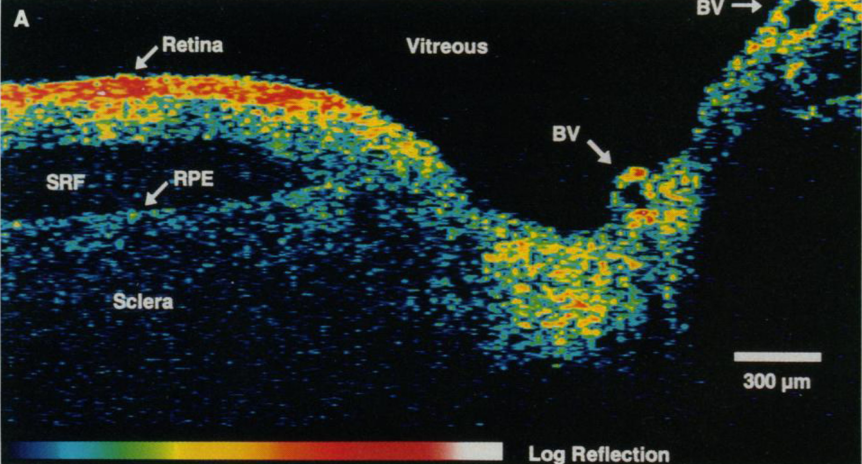
\includegraphics[width=.45\linewidth]{gfx/ch1/huang-eye}} \quad
\subfloat[Histology]
{\label{fig:huang-hist-sub}
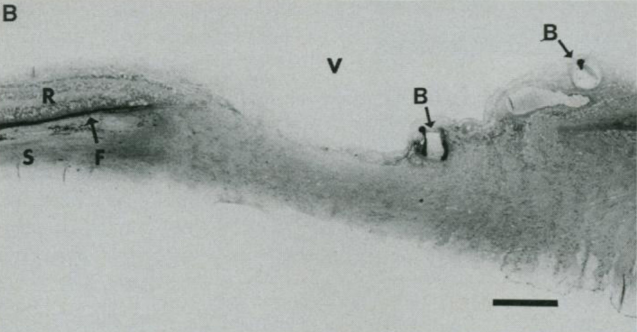
\includegraphics[width=.45\linewidth]{gfx/ch1/huang-histology}}\\
\subfloat[SSOCT]
{\label{fig:dhallaeyessoctsub}
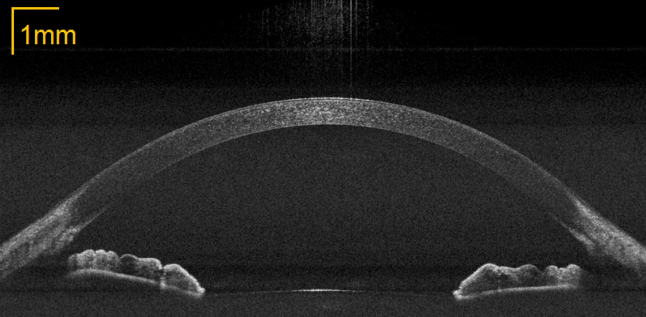
\includegraphics[width=.65\linewidth]{gfx/ch1/dhalla-eye-ssoct-2}}\\
\caption[OCT and histological images of the human eye.]{Optical coherence tomograph of human retina and optic disk in vitro (top left) and histologic section of the same sample (top right) \citep{Huang1991}. On the bottom, a \ac{SS-OCT} image of a live human eye sample \citep{Dhalla2012}. }\label{fig:huang-oct-vs-histology}
\end{figure}


The first drawback of OCT as a medical imaging technique comes from its relatively low imaging penetration, which is usually between less than a millimeter up to a couple of centimeter, depending on the specific technology and the absorption coefficient of the sample to analyse. In \autoref{fig:imaging-techniques-comparison}, a comparison between OCT, Ultrasound, and Confocal Microscopy is available \citep{Drexler2015}. The trend is that for an increasingly better imaging resolution, imaging depth has to be sacrificed. In this aspect, OCT sits right between the other two techniques, offering micrometer-level resolution for a moderate image penetration. \\

\begin{figure}[htb]
\myfloatalign
{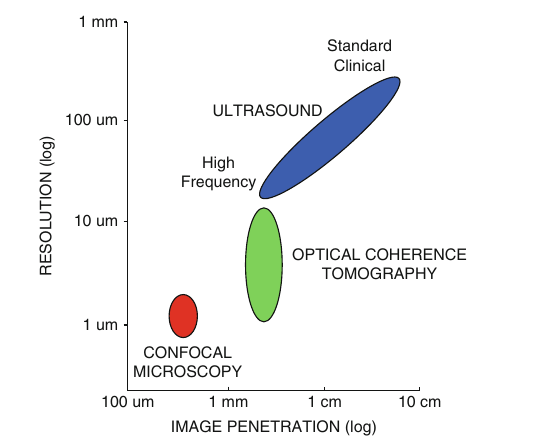
\includegraphics[width=.7\linewidth]{gfx/ch1/techniques-comparison}}
\caption{Imaging resolution and image penetration compared for different imaging techniques.}\label{fig:imaging-techniques-comparison}
\end{figure}

\begin{table}
\myfloatalign
\begin{tabularx}{\textwidth}{Xllll} \toprule
    \tableheadline{Source} & \tableheadline{Year} & \tableheadline{Voxels} & \tableheadline{Vol. Rate} & \tableheadline{Speed} \\
                           &  &  & {\scriptsize Volumes/s} & {\scriptsize GVoxels/s} \\ \midrule
    \citeauthor{Zhang10}\cite{Zhang10}             & 2010 & 6400000    & 10    & 0.06 \\
    \citeauthor{Choi2012} \cite{Choi2012}           & 2012 & 4194304    & 41    & 0.17 \\
    \citeauthor{Wieser14} \cite{Wieser14}           & 2014 & 40960000   & 26    & 1.07 \\
    \citeauthor{Darbrazi2016} \cite{Darbrazi2016}   & 2016 & 1408800000 & 2.05  & 2.89 \\
\bottomrule
\end{tabularx}
\caption{Performance of different implementations of volumetric OCT using GPGPU (adapted from \citep{Darbrazi2016}).}
\label{tab:volume-performance}
\end{table}


Whenever cross-sectional images are not sufficient for a correct diagnosis, volumetric data can be exploited for a more in-depth analysis. Volumetric images are composed by multiple 2D images captured in succession along a certain scanning direction, creating a 3D grid of datapoints called Voxels. \marginpar{A voxel is the primary unit of three-dimensional datasets, like the pixel is for 2D data. The word voxel originated by analogy with the word "pixel", with vo representing "volume" and el representing "element"} Two examples of 3D-OCT data obtained with SS-OCT (left) \citep{Dhalla2012} and SD-OCT (right) \citep{Choi2012} are depicted in \autoref{fig:3d-example}. 

With the near-exponential growth in computing power over the last decades, and the advent of \ac{GPU} computing by means of the \ac{GPGPU} paradigm, advanced volume rendering and signal-processing algorithms can be applied on large OCT data sets in real-time. In \autoref{tab:volume-performance} a few results from the literature are summarized, highlighting the advancement in processing power using GPU solutions (adapted from \citep{Darbrazi2016}).

Starting from 3D-OCT data it is also possible to generate \emph{en-face} projections of the sample at different depths, providing an invaluable tool for further analysis. A result of this technique is available in \autoref{fig:en-face-example}, which shows a frontal view of the macula, the central part of the retina, affected by an edema.

\begin{figure}[hbt]
\myfloatalign
\subfloat[Human eye]
{\label{fig:3d-example-a}
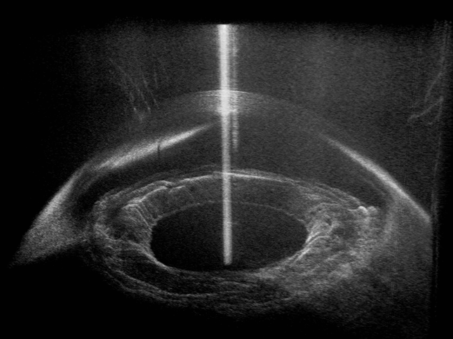
\includegraphics[height=4.5cm]{gfx/ch1/dhalla-eye-3d}} \quad
\subfloat[Human finger]
{\label{fig:3d-example-b}
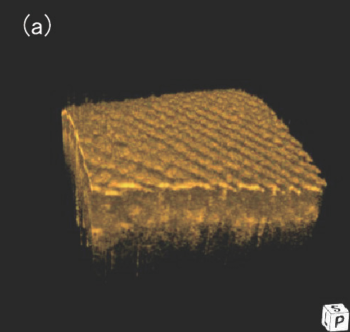
\includegraphics[height=4.5cm]{gfx/ch1/choi-finger-3d}}\\
\caption{Example of 3D OCT data: human eye obtained with SS-OCT \citep{Dhalla2012} (left) and human finger obtained with SD-OCT \citep{Choi2012} (right).}\label{fig:3d-example}
\end{figure}

\begin{figure}[hbt]
	\myfloatalign
		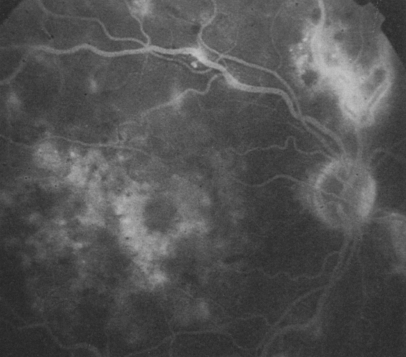
\includegraphics[width=0.45\linewidth]{gfx/ch1/en-face}
	\caption{En-face view for the assessment of macular edema \cite{MichaelRHee1995}.}\label{fig:en-face-example}
\end{figure}

% APPLICATIONS
\section{Applications}
\subsection{Medicine}
\marginpar{Angiography or arteriography is a medical imaging technique used to visualize the inside, or lumen, of blood vessels and organs of the body}
Ophtalmic applications have already been briefly mentioned in \autoref{sec:intro}, but other areas of medicine such as Cardiology \citep{Jang604,Bouma317} and Angiography \citep{Spaide2015,Jia2014} have benefitted from the diagnostic capabilities of OCT. A comparison between OCT and Ultrasound images of a coronary plaque is available in \autoref{fig:coronary}: the higher resolution of the optical system is substantial.



\begin{figure}[hbt]
	\myfloatalign
	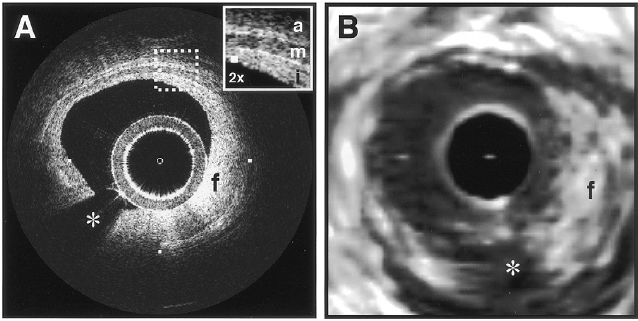
\includegraphics[height=4.5cm]{gfx/ch1/oct-vs-ultrasound-endoscopy}
	\caption{Coronary plaque imaged by OCT (left) and  \acf{IVUS} (right) \citep{Jang604}.}\label{fig:coronary}
\end{figure}


These applications are made possible by the small footprint of optical fibers (in the order of 200 $\mu$m of diameter) and the use of \ac{MEMS} mirrors, which can be easily embedded in endoscopes, catheters or other special probes \citep{Tearney96,Liao2017}. An example of a focus-adjustable probe is depicted in \autoref{fig:oct-endoscope}.

\begin{figure}[hbt]
	\myfloatalign
	\subfloat[Scheme.]
	{\label{fig:endoscope-scheme}
		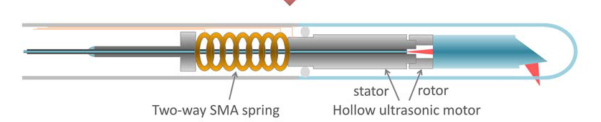
\includegraphics[width=0.55\linewidth]{gfx/ch1/endoscope-scheme}} \\
	\subfloat[Real life model.]
	{\label{fig:endoscope-real}
		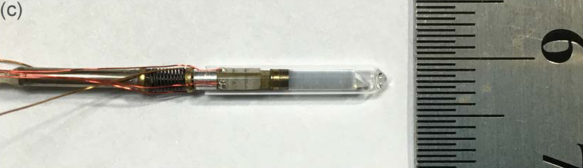
\includegraphics[width=0.55\linewidth]{gfx/ch1/endoscope-real}}\\
	\caption{Probe for endoscopic OCT \cite{Liao2017}.}\label{fig:oct-endoscope}
\end{figure}

\ac{EOCT} became an important tool for the detection of cancers affecting different parts of the human body, including bladder \citep{Xie2003}, cervix \citep{Escobar2004} and colon \citep{Hariri2006}. 
Other applications in the field of medicine include dermatology \citep{Korde2007,GAMBICHLER2005} and dentistry \citep{Amaechi2001,Machoy2017}. Low-delay, real-time OCT systems are also employed as a guidance tool for surgeries or tissue removal \cite{Boppart1999,Boppart2004}, allowing micrometer-scale resolution and providing depth-resolved images which are unobtainable with other classical methods.

\subsection{Industrial}
OCT has also found widespread application in a variety of non-medical fields, especially where non-contact, high-precision measurements are needed. For example, real-time monitoring and thickness measurement of multi-layer structures are important tools in the manufacturing of microelectronics and optical devices. Industrial uses of OCT range from defect detection in ceramic and polymeric materials \cite{Wiesauer2005,Su2014} to quality evaluation of paper products \cite{Prykari2010,Alarousu2005}. An interesting usage is found in \cite{Liang2005}, where the non-invasive examination of museum paintings was demonstrated, paving the way for OCT to the field of art conservation.

\begin{figure}[hbt]
	\myfloatalign
	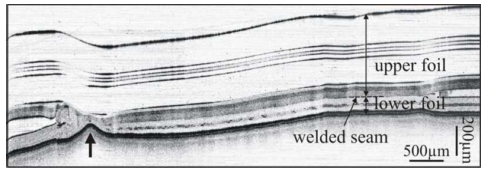
\includegraphics[width=0.5\linewidth]{gfx/ch1/material}
	\caption{Cross-sectional OCT image of a multi-layered plastic foil used in the food packaging industry \citep{Wiesauer2005}.}\label{fig:material}
\end{figure}

\subsection{In vivo monitoring of biological specimen}
We've seen that non-destructive measurements are essential in human medical diagnostic, but in vivo cross-sectional analysis is suited for a wide range of other biological samples. OCT has been used for growth monitoring of seeds \cite{Ravichandran2017}, virus detection in plants \cite{Chow2009}, and even quality assessment of egg quality in the poultry industry \cite{Sabuncu2015}. Alternative methods such as histology, \ac{SEM} imaging, \ac{MRI} and X-Ray radiography are either distructive or can not guarantee the possibility of continuous monitoring with a comparable image resolution.

\begin{figure}[hbt]
	\myfloatalign
	\subfloat[Plant seeds]
	{\label{fig:seeds}
		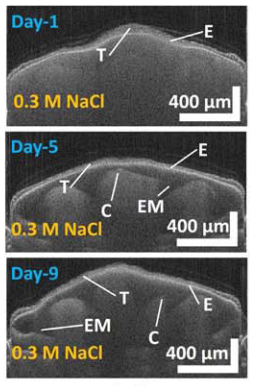
\includegraphics[height=2.5cm]{gfx/ch1/seeds}} \quad
	\subfloat[Lettuce leaf]
	{\label{fig:lettuce}
		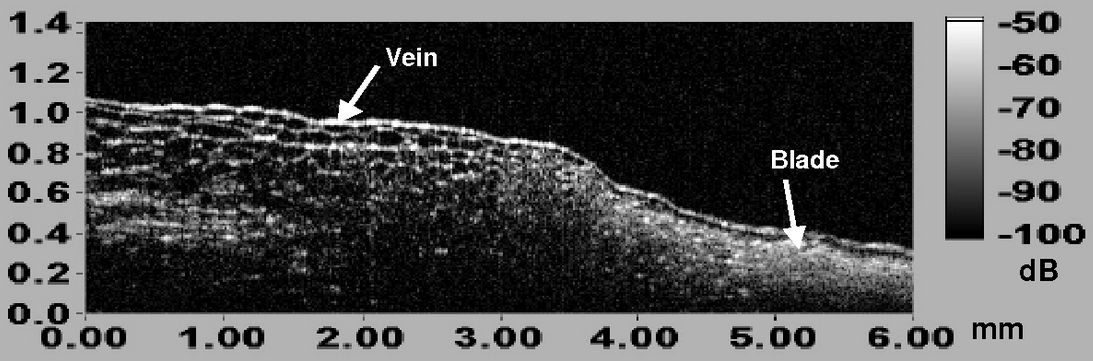
\includegraphics[height=2.5cm]{gfx/ch1/lettuce}}\\
	\caption{Growth monitoring of \emph{Capsicum annuum seeds} \cite{Ravichandran2017} (left) and lettuce leaf \cite{Loeb2003} (right).}\label{fig:plant-monitoring}
\end{figure}

\subsection{Functional imaging}
Apart from the structural imaging of biological tissue, OCT can also be utilized to perform \emph{functional} imaging, giving the user insights on the different properties of the material under analysis. \ac{PS-OCT} schemes can measure properties such as birefringence, dichroism and optic axis orientation of the sample \cite{DeBoer1997}, while \ac{DOCT} and \ac{svOCT} are able to estimate the direction and velocity of the blood flow in vessels \cite{Mahmud2013}. Birefringence measurement has found use in dentistry, specifically in the monitoring of caries lesions and their progression, enabling early detection and preventing the need for surgical intervention \cite{Fried2002}. 

\section{Objectives}
The study conducted in this thesis is based on a previous thesis \cite{Calabrese2017} developed in the \ac{PEG} Laboratory at the \ac{DEI} of the University of Padova. It consisted in the preliminary characterization of the main components of a high speed \acf{SS-OCT} system working in the 1300 nm range and the experimental determination of different parameters of the device, such as the source coherence length, the achievable scanning speed and the transversal resolution permitted by the focusing optics. \\

\noindent The primary objectives of this thesis are the following:
\begin{enumerate}
	\item Designing and testing the optical circuitry needed for a stable SS-OCT system.
	\item Developing a \ac{DAQ} application capable of continuous and low-delay video stream.
	\item Control and synchronization of the Galvanometric System with the optical source and the \ac{DAQ} board. 
	\item Acquiring cross-sectional and volumetric data of different samples.
\end{enumerate}

\section{Thesis Structure}
The structure of this document is organized in the following manner:
\begin{itemize}
	\item \autoref{ch:theory} consists of the theoretical background on the electromagnetic phenomena of interference and temporal coherence. The basic operating principle of different OCT schemes will be thoroughly detailed. 
	\item In \autoref{ch:setup} I will give a description of the optical and electrical devices that were used for the implementation of the final SS-OCT system. Additionally, the methods that were employed for its design and for the characterization of its performance will be reviewed. 
	\item \autoref{ch:results} is dedicated to a comprehensive explanation of the OCT software that was created to acquire and visualize OCT images in real-time. It will also showcase a series of cross-sectional images and basic volume renderings obtained from a variety of different samples. 
	\item \autoref{ch:conclusions} concludes the thesis, illustrating possible future developments and further improvements of the presented work.  
\end{itemize}


% \begin{figure}[hbt]
% \myfloatalign
% \documentclass{standalone}


\usepackage[osf,sc]{mathpazo}
\linespread{1.05}
  \usepackage{pgfplots}
  \usepackage[euler-digits]{eulervm}
  \pgfplotsset{compat=newest}
  %% the following commands are needed for some matlab2tikz features
  \usetikzlibrary{plotmarks}
  \usetikzlibrary{arrows.meta}
  \usepgfplotslibrary{patchplots}
  \usepackage{grffile}
  \usepackage{amsmath}
  

  %% you may also want the following commands
  %\pgfplotsset{plot coordinates/math parser=false}
  %\newlength\figureheight
  %\newlength\figurewidth

\begin{document}
  \documentclass{standalone}


\usepackage[osf,sc]{mathpazo}
\linespread{1.05}
  \usepackage{pgfplots}
  \usepackage[euler-digits]{eulervm}
  \pgfplotsset{compat=newest}
  %% the following commands are needed for some matlab2tikz features
  \usetikzlibrary{plotmarks}
  \usetikzlibrary{arrows.meta}
  \usepgfplotslibrary{patchplots}
  \usepackage{grffile}
  \usepackage{amsmath}
  

  %% you may also want the following commands
  %\pgfplotsset{plot coordinates/math parser=false}
  %\newlength\figureheight
  %\newlength\figurewidth

\begin{document}
  \input{falloff-fit.tikz}
\end{document}

\end{document}

% \caption[]{Example of 3D OCT data: human eye obtained with SS-OCT \citep{Dhalla2012} (left) and human finger obtained with SD-OCT \citep{Choi2012} (right).}\label{fig:3d-example}
% \end{figure}

% \begin{figure}[hbt]
% \myfloatalign
% \documentclass{standalone}


\usepackage[osf,sc]{mathpazo}
\linespread{1.05}
  \usepackage{pgfplots}
  \usepackage[euler-digits]{eulervm}
  \pgfplotsset{compat=newest}
  %% the following commands are needed for some matlab2tikz features
  \usetikzlibrary{plotmarks}
  \usetikzlibrary{arrows.meta}
  \usepgfplotslibrary{patchplots}
  \usepackage{grffile}
  \usepackage{amsmath}
  

  %% you may also want the following commands
  %\pgfplotsset{plot coordinates/math parser=false}
  %\newlength\figureheight
  %\newlength\figurewidth

\begin{document}
  \documentclass{standalone}


\usepackage[osf,sc]{mathpazo}
\linespread{1.05}
  \usepackage{pgfplots}
  \usepackage[euler-digits]{eulervm}
  \pgfplotsset{compat=newest}
  %% the following commands are needed for some matlab2tikz features
  \usetikzlibrary{plotmarks}
  \usetikzlibrary{arrows.meta}
  \usepgfplotslibrary{patchplots}
  \usepackage{grffile}
  \usepackage{amsmath}
  

  %% you may also want the following commands
  %\pgfplotsset{plot coordinates/math parser=false}
  %\newlength\figureheight
  %\newlength\figurewidth

\begin{document}
  \input{falloff.tikz}
\end{document}

\end{document}

% \caption[]{Example of 3D OCT data: human eye obtained with SS-OCT \citep{Dhalla2012} (left) and human finger obtained with SD-OCT \citep{Choi2012} (right).}\label{fig:3d-example}
% \end{figure}

% \begin{figure}[hbt]
% \myfloatalign
% \documentclass{standalone}


\usepackage[osf,sc]{mathpazo}
\linespread{1.05}
  \usepackage{pgfplots}
  \usepackage[euler-digits]{eulervm}
  \pgfplotsset{compat=newest}
  %% the following commands are needed for some matlab2tikz features
  \usetikzlibrary{plotmarks}
  \usetikzlibrary{arrows.meta}
  \usepgfplotslibrary{patchplots}
  \usepackage{grffile}
  \usepackage{amsmath}
  

  %% you may also want the following commands
  %\pgfplotsset{plot coordinates/math parser=false}
  %\newlength\figureheight
  %\newlength\figurewidth

\begin{document}
  \documentclass{standalone}


\usepackage[osf,sc]{mathpazo}
\linespread{1.05}
  \usepackage{pgfplots}
  \usepackage[euler-digits]{eulervm}
  \pgfplotsset{compat=newest}
  %% the following commands are needed for some matlab2tikz features
  \usetikzlibrary{plotmarks}
  \usetikzlibrary{arrows.meta}
  \usepgfplotslibrary{patchplots}
  \usepackage{grffile}
  \usepackage{amsmath}
  

  %% you may also want the following commands
  %\pgfplotsset{plot coordinates/math parser=false}
  %\newlength\figureheight
  %\newlength\figurewidth

\begin{document}
  \input{clock.tikz}
\end{document}

\end{document}

% \caption[]{Example of 3D OCT data: human eye obtained with SS-OCT \citep{Dhalla2012} (left) and human finger obtained with SD-OCT \citep{Choi2012} (right).}\label{fig:3d-example}
% \end{figure}

% \begin{figure}[hbt]
% \myfloatalign
% \input{gfx/clock-1.tikz}
% \caption[]{Example of 3D OCT data: human eye obtained with SS-OCT \citep{Dhalla2012} (left) and human finger obtained with SD-OCT \citep{Choi2012} (right).}\label{fig:3d-example}
% \end{figure}

% \begin{figure}[hbt]
% \myfloatalign
% \input{gfx/clock-2.tikz}
% \caption[]{Example of 3D OCT data: human eye obtained with SS-OCT \citep{Dhalla2012} (left) and human finger obtained with SD-OCT \citep{Choi2012} (right).}\label{fig:3d-example}
% \end{figure}

% \begin{figure}[hbt]
% \myfloatalign
% \input{gfx/frequency-estimation.tikz}
% \caption[]{Example of 3D OCT data: human eye obtained with SS-OCT \citep{Dhalla2012} (left) and human finger obtained with SD-OCT \citep{Choi2012} (right).}\label{fig:3d-example}
% \end{figure}

% \begin{figure}[bth]
% \myfloatalign
% {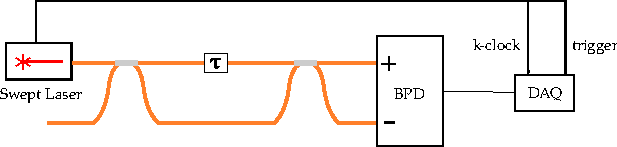
\includegraphics[width=\linewidth]{gfx/interferometer.pdf}}
% \caption{En vivo measurement of rabbit's eyeball.}
% \end{figure}


% \begin{figure}[bth]
% \myfloatalign
% {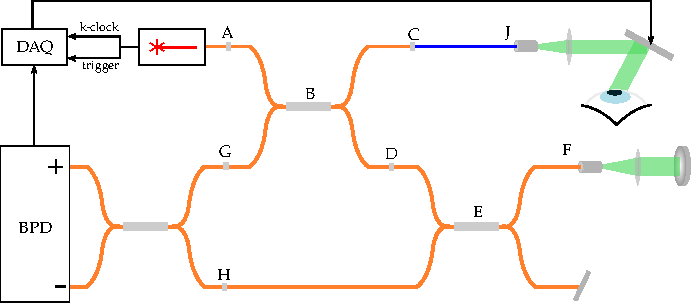
\includegraphics[width=\linewidth]{gfx/final-setup.pdf}}
% \caption{En vivo measurement of rabbit's eyeball.}
% \end{figure}

% \begin{figure}[bth]
% \myfloatalign
% {\includegraphics[width=.75\linewidth]{gfx/ch1/fujimoto-rabbit}}
% \caption{En vivo measurement of rabbit's eyeball.}
% \end{figure}

% \begin{figure}[bth]
% \myfloatalign
% \subfloat[Asia personas duo.]
% {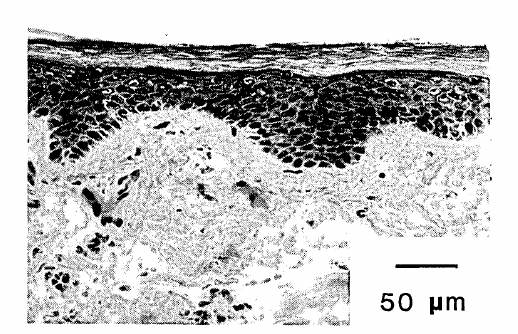
\includegraphics[width=.55\linewidth]{gfx/ch1/fujimoto-histology}} \quad
% \subfloat[Pan ma signo.]
% {\label{fig:example-b}
% 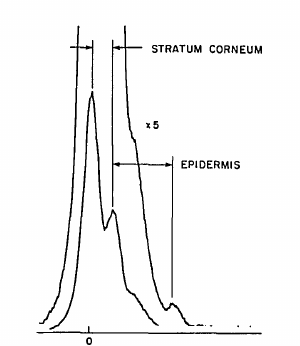
\includegraphics[width=.35\linewidth]{gfx/ch1/fujimoto-ascan}}
% \caption[Tu duo titulo debitas latente]{Tu duo titulo debitas latente.}\label{fig:example}
% \end{figure}

% Chapter 2

\chapter{Basic Theory of Optical Coherence Tomograpy} % Chapter title
\label{ch:theory} % For referencing the chapter elsewhere, use \autoref{ch:examples} 

In this chapter I will report the basic theoretical background needed to comprehend the working mechanisms behind the OCT technique, introduce the different schemes and compare them in terms of performance. The content of this chapter is partially adapted from \cite{Midrio2006,Someda2006,Wolf1999}. 


\section{Principles of Coherence and Interference}
A solution to a generic electromagnetic problem is completely determined by the vector couple $\mathcal{S} = \left\{\mathbf{E}(\mathbf{r}, t),\; \mathbf{H}(\mathbf{r}, t)\right\}$, whose components represent the time-varying electric and magnetic field at a specific point $\textbf{r}$  in space. The electromagnetic field determined by $\mathcal{S}$ is considered a valid solution if it satisfies both Maxwell's Equations and the boundary conditions specific to the problem. 

For monochromatic waves, i.e. fields oscillating at a single frequency $\omega$, we can use Steinmetz notation and write
\begin{equation}\label{eq:steinmetz}
	\textbf{E}(\textbf{r}, t) = \Re\left[\widetilde{\mathbf{E}}(\textbf{r})e^{j\omega t}\right] \qquad \textbf{H}(\textbf{r}, t) = \Re\left[\widetilde{\mathbf{H}}(\textbf{r})e^{j\omega t}\right]\,,
\end{equation}
where $\widetilde{\textbf{E}}$ and $\widetilde{\textbf{H}}$ are complex 3D vectors and $\Re\left[\cdot\right]$ is the real value operator. In a linear, homogeneous, isotropic, and current-free medium, Maxwell's equations can be written in the frequency domain in the following way

\begin{subequations}\label{eq:maxwell-frequency}
\begin{align}
& \nabla \times \widetilde{\textbf{E}} = -j\omega\mu\widetilde{\textbf{H}} \label{eq:maxwell-e}\\
& \nabla \times \widetilde{\textbf{H}} = j\omega\varepsilon_c\widetilde{\textbf{E}}\label{eq:maxwell-h}
\end{align}
\end{subequations}
where $\mu$ is the magnetic permeability of the medium, $\varepsilon_c = \varepsilon - \sigma/\omega$ is the complex dielectric permettivity and $\sigma$ is the conductivity. The simplest solution of \autoref{eq:maxwell-frequency} is given by the \emph{homogeneous plane wave}. Using a cartesian coordinate system, the electric field can be expressed as
\begin{equation}\label{eq:e-field-expansion}
		\widetilde{\textbf{E}}(\textbf{r}) = \sum_{i=1}^3 A_i \cdot \hat{\textbf{x}}_i  = \sum_{i=1}^3 a_i \exp\left[jg_i(\textbf{r})\right]  \cdot \hat{\textbf{x}}_i
\end{equation}
where the amplitudes $a_i$ are constant and $g_i(\textbf{r}) = \textbf{k}\cdot\textbf{r} - \delta_i$ represent the phase functions of the electric field components. The propagation vector $\textbf{k}$ is given as a function of the wavelength $\lambda$ as follows
\begin{equation}
	|\textbf{k}| = \frac{2\pi}{\lambda},
\end{equation}
while the $\delta_i$'s are the phase differences which determine the state of polarization of the electromagnetic field. The magnetic field is instead obtained by applying \autoref{eq:maxwell-e} to \autoref{eq:e-field-expansion}. 

The intensity of an electromagnetic field is given by the average amount of energy which crosses in a unit time a unit area perpendicular to the direction of the energy flow. In the case of homogenous plane waves, it is expressed as
\begin{equation}\label{eq:intensity}
	I \propto \langle \textbf{E}^2 \rangle
\end{equation}

Using \autoref{eq:steinmetz}, we can express the electric field as
\begin{equation}\label{eq:e-steinmetz}
\textbf{E}(\textbf{r}, t) = \frac{1}{2}\left[ \widetilde{\textbf{E}}(\textbf{r})e^{-j\omega t} + \widetilde{\textbf{E}}^*(\textbf{r})e^{j\omega t}\right],
\end{equation}
so that \autoref{eq:intensity} can be written as
\begin{equation}
	\langle\textbf{E}^2\rangle = \frac{1}{4} \left\langle\widetilde{\textbf{E}}^2 e^{-2j\omega t} + \widetilde{\textbf{E}}^{*2}e^{2j\omega t} + 2  \widetilde{\textbf{E}}\cdot\widetilde{\textbf{E}}^*\right\rangle \,.
\end{equation}
Averaging over a time interval sufficiently larger than the period $T=2\pi/ \omega$, we obtain
\begin{equation}
	\langle \textbf{E}^2 \rangle =\frac{1}{2}\widetilde{\textbf{E}}\cdot\widetilde{\textbf{E}}^* =\frac{1}{2}\left(a_1^2 + a_2^2 + a_3^2\right) = \text{constant},
\end{equation}
as the high frequency terms at $2\omega$ are canceled by the detector.

Suppose now that the field $\textbf{E}$ is split in two components $\textbf{E}_1$ and $\textbf{E}_2$ which are then superimposed in a certain point $\textbf{r}'$ in space, then
\begin{equation}
\textbf{E}(\textbf{r}') = \textbf{E}_1(\textbf{r}') + \textbf{E}_2(\textbf{r}'),
\end{equation}

which implies that
\begin{equation}
	\textbf{E}^2 (\textbf{r}')= \textbf{E}_1^2(\textbf{r}') + \textbf{E}_2^2(\textbf{r}') + 2\textbf{E}_1(\textbf{r}')\cdot\textbf{E}_2(\textbf{r}')
\end{equation}

The field intensity is thus
\begin{equation}\label{eq:intensity-interference}
I = I_1 + I_2 + J_{12} = \langle\textbf{E}_1^2\rangle + \langle\textbf{E}_2^2\rangle + 2\langle\textbf{E}_1\cdot\textbf{E}_2\rangle.
\end{equation}
The last term in \autoref{eq:intensity-interference} is called \emph{interference}. Depending on the phase difference between the two fields, the total intensity can assume different values.  If the difference between the optical paths traveled by the two components is $\Delta z$, the phase difference will be $\delta = \Delta z \cdot 2\pi/\lambda $, and the interference term will be equal to
\begin{equation}
	J_{12} = 2\langle\textbf{E}_1\cdot\textbf{E}_2\rangle = \left(a_1^2 + a_2^2 + a_3^2\right)\cos\delta.
\end{equation}
In the simple case in which the two fields are linearly polarized along the $\textbf{x}_1$ direction, we have that $a_2 = a_3 = 0$, and $I_1 = I_2 = 1/2\, a_1^2$, while the interference is
given by $J_{12} = a_1^2\cos\delta = 2\sqrt{I_1 I_2}\cos \delta$. 
The total intensity is then
\begin{equation}
	I = I_1 + I_2 + 2 \sqrt{I_1I_2}\cos\delta = 2I_1 + 2I_1\cos\delta \in [0, 4I_1].
\end{equation}
The intensity profile is displayed in \autoref{fig:intensity-interference}. In this first approximation of perfectly monochromatic waves there are no constraint on the phase offset $\delta$ or on the optical path difference $\Delta z$ for the presence of intereference. 

\begin{figure}[hbt]
	\myfloatalign
	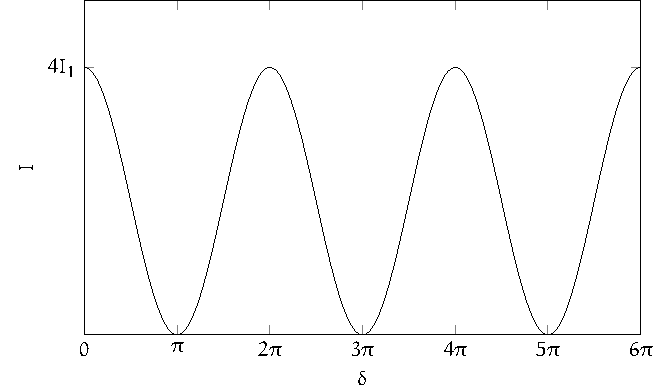
\includegraphics[width=0.8\linewidth]{gfx/tikz/interference.pdf}
	\caption{Interference fringes created by two beams of equal intensity.}\label{fig:intensity-interference}
\end{figure}

\subsection{Michelson interferometer}
\label{sub:michelson}
A classical example of the application of interference is given by the scheme called \emph{Michelson interferometer}, whose schematic diagram is available in \autoref{fig:michelson}. A light source emits an electric field $\textbf{E}_0$ which is then split in two by a semitransparent mirror. The two replicas, $\textbf{E}_1$ and $\textbf{E}_2$, travel along the two \emph{arms} of the interferometer, of length $l_1$ and $l_2$, are reflected by two mirrors and finally recombined. The intensity of the superposition of two fields is then measured by a photodetector. The two replicas arrive at the detector with a time difference given by
\begin{equation}
	\tau = 2\frac{l_2 - l_1}{c},
\end{equation}
where $c$ is the speed of light in the considered medium. From \autoref{eq:intensity-interference} we then obtain
\begin{align}\label{eq:michelson-intensity}
	I &= I_1 + I_2 + 2 \langle\textbf{E}_1(t) \cdot \textbf{E}_2(t)\rangle =  2 \left[I_1 + \langle\textbf{E}_1(t) \textbf{E}_1(t-\tau) \rangle\right]\\
	 &= 2I_1\left\{ 1 + \cos\left[\frac{2\pi}{\lambda}2(l_2-l_1)\right]\right\}.
\end{align}

%\todo{Expand this formula defining the degree of coherence so that it's easier to describe TDOCT signals}

\begin{figure}[hbt]
	\myfloatalign
	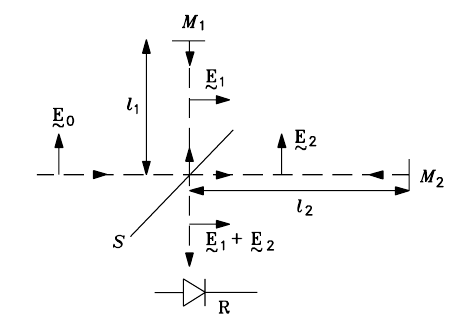
\includegraphics[width=0.7\linewidth]{gfx/michelson}
	\caption{Diagram of a Michelson interferometer \cite{Someda2006}. }\label{fig:michelson}
\end{figure}

This type of interferometer can be used to perform high-precision measurements of distances by making one of the arms mobile and mantaining the other fixed as a reference. Counting the number of "peaks" and "valleys" of the intensity profile as the mobile arm is translated, an estimate of path length difference is given with a precision of $\lambda/2$. \\


\subsection{Fringe visibility}

\noindent We can define a useful parameter called \emph{fringe visibily} as follows
\begin{equation}
\label{eq:fringevisibily}
v = \frac{I_{max} - I_{min}}{I_{max} + I_{min}}.
\end{equation}


For a perfectly monochromatic source, $v$ will always be constant. In particular, in the case when $I_1 = I_2$  $v$ is equal to 1, as $I_{min} = 0$. Real-life optical sources however will always have a bandwidth $\Delta f$ greater than 0 due to random fluctuations of the electromagnetic radiation. In these cases $v$ is a monotonically decreasing function of the time delay $\tau$.  The \emph{coherence time} of a source is defined as the value $\tau_c$ such that $v(\tau_c) = 1/e$ (\autoref{fig:fringe-visibility}). 




\begin{figure}[hbt]
	\myfloatalign
	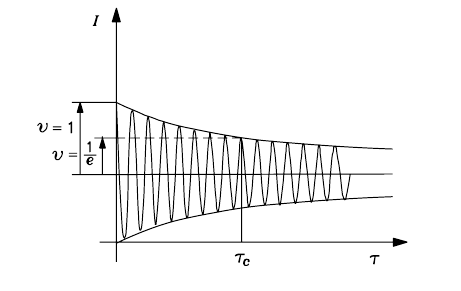
\includegraphics[width=0.8\linewidth]{gfx/fringe-visibility}
	\caption{Effect of the coherence time of a source on the interference fringes at the output of a Michelson interferometer \cite{Someda2006}.}\label{fig:fringe-visibility}
\end{figure}


Intuitively, we may think of the coherence time as the time slot after which the optical source loses memory of what it was at the beginning. In fact, after this time slot has passed, some properties of the source randomly change due to the stochastic nature of photon emission. A perfectly coherent source emits a sinusoidal field with a well defined and constant phase relation. Similarly, two electromagnetic fields are perfectly coherent if the phase difference between the two is mantained constant for an infinite amount of time. This property is however impossible to obtain in real life, as every source has a finite coherence time.
\subsection{The coherence function}
Another way to describe the coherence property of light other than the fringe visibility parameter, is through the so-called \emph{mutual coherence function}. It is defined for polychromatic, i.e., non-monochromatic fields as follows \cite{Wolf1999}:
\begin{equation}\label{eq:mutual-coherence}
	\Gamma_{12}(\tau) = \left\langle  \mathbf{E}_1(t+\tau)\mathbf{E}_2^*(t)   \right\rangle,
\end{equation}
If $\mathbf{E}_1 = \mathbf{E}_2$, it is called \emph{self-coherence function}, and it's written as $\Gamma_{11}(\tau)$. Notice that when $\tau = 0$ it reduces to the field intensity:
\begin{equation}
	\Gamma_{ii}(0) = I_i\,.
\end{equation}
It is then useful to apply the following normalization
\begin{equation}
	\gamma_{ij} (\tau) = \frac{\Gamma_{ij}(\tau)}{\sqrt{\Gamma_{ii}(0)}\sqrt{\Gamma_{jj}(0)}},
\end{equation}
so that the function assumes values in the $[0,1]$ interval. This normalized function is called \emph{complex degree of coherence}, and it allows the following definitions:
\begin{enumerate}
	\item Completely incoherent fields: $|\gamma_{ij}| = 0$, no interference fringes are visible.
	\item Completely coherent fields: $|\gamma_{ij}| = 1$, the total intensity includes the interference term. 
	\item Partially coherent fields: $0 < |\gamma_{ij}| < 1$, interference fringes are present, and assume a visibility parameter equal to 
	\begin{equation}
		v = \frac{2\sqrt{I_i I_j}}{I_i + I_j}|\gamma_{ij}|.
	\end{equation}
	When the two fields have equal intensity the two parameters coincide.
\end{enumerate}

Using this notation, the equation for the intensity of two partially-coherent beams is then
\begin{equation}
	I = I_1 + I_2 + 2\sqrt{I_1I_2}|\gamma_{12}(\tau)| \cos( \delta + \angle \gamma_{12}(\tau) )\,
\end{equation}
where we can clearly see the effect of coherence on the shaping of the interference fringes. Using the coherence function instead of the fringe visibility as a measure of coherence, the coherence time of a source, $\tau_c$, is defined as the \ac{FWHM} parameter of its self-coherence function, that is, the value of $\tau$ such that
\begin{equation}
	|\gamma(\tau)| = \frac{|\gamma(0)|}{2}.
\end{equation}

The shape of the coherence function of an optical source is completely determined by its spectrum $I(k)$ through the Wiener-Khintchine theorem, which states that the autocorrelation function and the \ac{PSD} of a random process are connected through their Fourier Transform. 




\subsection{Coherence length}

Starting from the coherence time of the source, $\tau_c$, we can also define its coherence length as follows
\begin{equation}
	l_c = c_0 \tau_c,
\end{equation}
where $c_0 \simeq 3\cdot10^8$ m/s is the speed of light in vacuum. Using a light source with a coherence length $l_c$ in the Michelson interferometer previously presented, we would observe an interference pattern at the photoreceiver only if the difference in length of the two arms is such that 
\begin{equation}
\Delta l = |l_2 - l_1| \leq l_c / 2,
\end{equation}
or, equivalently, if the total \ac{OPD} is matched to within the coherence length of the source. 


While we just defined the coherence \emph{length} of a source, it's important to note that it is a parameter that is directly related to the time coherence and does not describe the phenomenon of spatial coherence. 

\section{OCT Terminology}
Before introducing the different OCT techniques it is useful to introduce some terminology that will be used throughout this thesis. The most basic OCT measure is called A-scan (Axial-scan), which is a signal that represents the reflectivity of a sample as a function of depth. The amount of information carried by these measurements is limited, but can be used to perform thickness measurements if the structure of the sample is known a priori. 

 \begin{figure}[hbt]
	\myfloatalign
	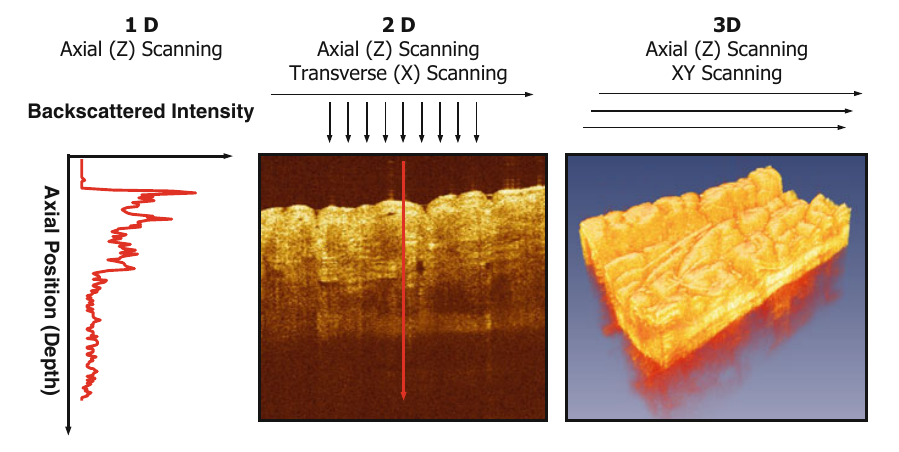
\includegraphics[width=\linewidth]{gfx/ch2/terminology}
	\caption{Diffent types of OCT measurements. \cite{Drexler2015}}\label{fig:terminology}
\end{figure}

If multiple consecutive A-scans are acquired along a transverse direction on the sample, a cross-sectional image, called B-scan, is generated. They are the most direct way to determine the anatomy of an unknown sample and are often sufficient for diagnostic purposes, especially in Ophtalmology. Their visualization does not require advanced techniques, but if a real-time high-resolution video stream is desired then careful design choices have to be made. 

Finally, 3D volumetric data can be generated by acquiring consecutive B-scans along a second direction on the transverse plane. Intuitively, they are called C-scans. Contrary to B-scans, volume rendering requires sophisticated and efficient algorithms for a correct data interpretation and visualization \cite{Lacroute1994,Cabral1994,Engel2001}. Starting from 3D data its also possible to obtain frontal projections of the sample, called \emph{en-face} views (\autoref{fig:enface}), or to generate cross-sections along an arbitrary plane.

 \begin{figure}[hbt]
	\myfloatalign
	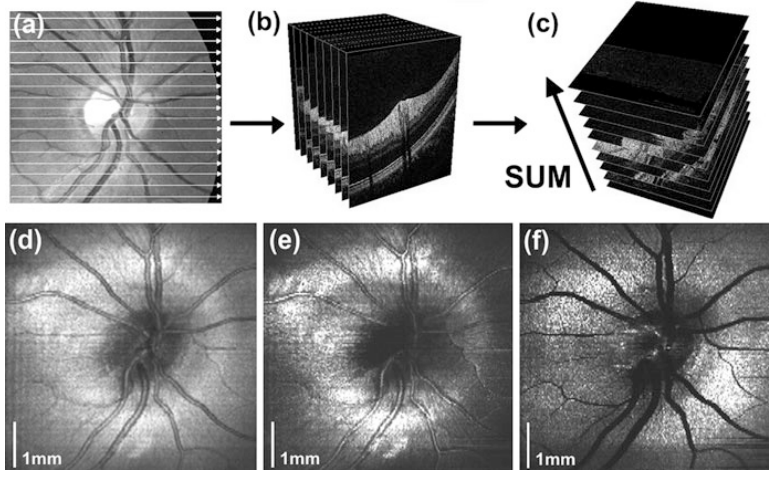
\includegraphics[width=\linewidth]{gfx/ch2/enface}
	\caption{\emph{En-face} view reconstructed from volumetric data\cite{Drexler2015}}\label{fig:enface}
\end{figure}

%The intensity profile given by \autoref{eq:michelson-intensity} can also be described through the \emph{coherence function} of the two fields, defined as
%\begin{equation}
%\Gamma_{ij}(\tau) = \left\langle  \textbf{E}_i(t)\cdot \textbf{E}_j(t+\tau)  \right\rangle,
%\end{equation}
%which gives
%\begin{equation}
%I = I_1 + I_2 + 2 \Re\left[\Gamma_{12}(\tau)\right] = I_1 + I_2 + 2 \Re\left[\Gamma_{21}(\tau)\right].
%\end{equation}
%
%In fact, since $\Gamma_{ii}(0) = I_i$, we can define the normalized coherence function as 
%\begin{equation}
%\gamma(\tau) = \frac{\Gamma(\tau)}{\Gamma(0)}
%\end{equation}




%In reality, eletromagnetic radiation consists in the emission of photons dictated by the decaying of atoms from a higher energy state to a lower energy state. The energy difference between these states, $E$, is directly proportional to the frequency $f$ of the emitted photon through Planck's constant $h$. The energy gap $E$ is however not uniquely defined, but is instead an interval of energies $\Delta E$, meaning that the frequency of the emitted photons will fall in a certain bandwidth $\Delta f = \Delta E / h$. 


%Copy from \cite{Wolf1999,Someda2006}

\section{Time Domain OCT}
 \acf{TD-OCT} is the first OCT technique that was demonstrated in the literature \cite{Huang1991}. The basic setup is that of a Michelson Interferometer in which one of the two mirrors is translatable and the other is replaced by the sample that we wish to analyze. The two arms are called respectively \emph{Reference arm} and \emph{Sample arm}. As explained in \autoref{sub:michelson}, the two beams arriving at the photodetector generate interference fringes if the \ac{OPD} is less than the coherence length $l_c$ of the source. A diagram of this setup is available in \autoref{fig:tdoct-michelson}. 
 
 
 \begin{figure}[hbt]
 	\myfloatalign
 	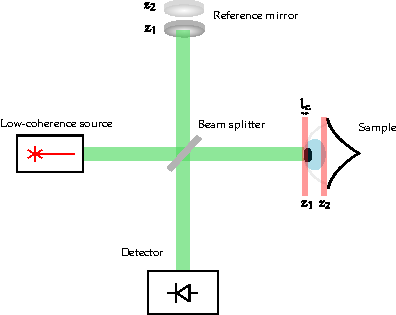
\includegraphics[width=0.8\linewidth]{gfx/tdoct}
 	\caption{Diagram of the basic \ac{TD-OCT} setup using a Michelson interferometer.}\label{fig:tdoct-michelson}
 \end{figure}
 
The light beam reflected by the reference mirror while in position $z_1$ will interfere with all the reflections occurring in the sample at depths $z \in [z_1 - l_c/2, z_1 + l_c/2]$. By measuring the intensity of the fringes it is then possible to obtain an estimate of the sample reflectivity at those depths. The whole axial measurement of the sample can be acquired by moving the translatable mirror along an adequate interval of positions. Since a single mirror position is mapped to an interval of length $l_c$ of axial positions in the sample, the coherence length of the source can be considered to be the axial resolution of the system. As a consequence short coherence lenghts are preferred, meaning that broadband sources are more widely employed. 

If the light source was perfectly monochromatic, the reference signal would interfere with an infinite number of reflected replicas generated at every depth in the sample, as there would be no constraint on the \ac{OPD}. 


To better understand this concept, suppose that the sample is an ideal reflector with a reflection coefficient $\rho_s$ is positioned in such a way that the \ac{OPD} is 0. The intensity measured by the detector when a \ac{OPD} equal to $\Delta z$ is introduced is then

\begin{align}\label{eq:tdoct-interference}
I(\Delta z) \propto |\rho_s|^2 |E_i|^2 + |\rho_r|^2 |E_i|^2 + |\rho_s\rho_r|^2|E_i|^2|\gamma(\Delta z)|\cos\left(\frac{2\pi}{\lambda_0}\Delta z\right)
\end{align}


\begin{figure}[hbt]
	\myfloatalign
	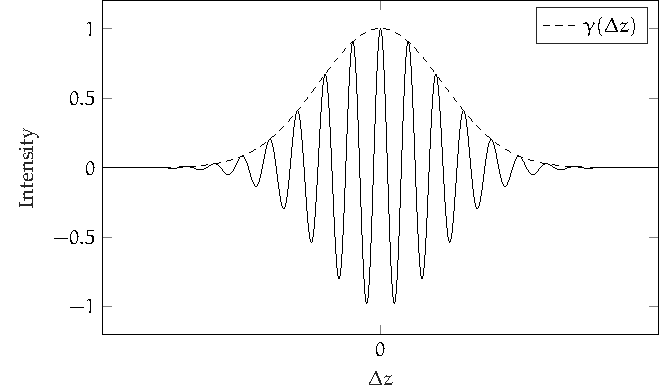
\includegraphics[width=0.8\linewidth]{gfx/tikz/tdoct-signal}
	\caption{Diagram of the basic \ac{TD-OCT} setup using a Michelson interferometer used in \cite{Huang1991}.}\label{fig:tdoct-signal}
\end{figure}


Apart from the DC offset given by the intensity of the two signals there is an oscillating term with period equal to $\lambda_0$, which is the central wavelength of the source. \autoref{fig:tdoct-signal} illustrates the oscillating term and its envelope, which is dictated by the coherence function $\gamma$ and the sample reflectivity $\rho_s$ (set equal to 1). With a perfectly coherent source $\gamma$ would be equal to 1 for all values of $\Delta z $ and we would not be able to identify the reflector. On the other hand, with an increasingly sharper $\gamma$, the ideal reflector would be more and more defined. 


Since the difference between the arm lengths is $\Delta l = \Delta z / 2$, when scanning the reference arm, interference fringes will be generated as a function of time with periodicity equal to $(\lambda/2) / \sigma$ where $\sigma$ is the mirror scanning speed. 

 
\begin{figure}[hbt]
	\myfloatalign
	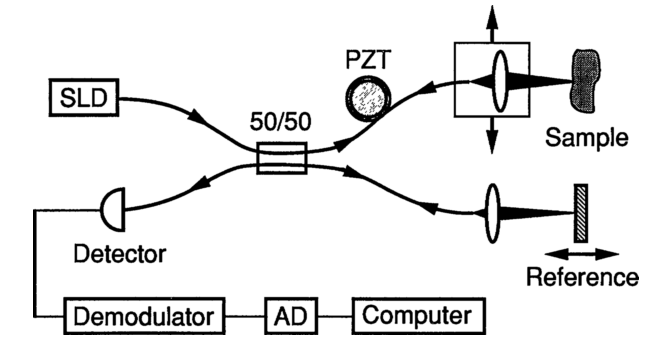
\includegraphics[width=0.8\linewidth]{gfx/ch2/huang-setup}
	\caption{Diagram of the basic \ac{TD-OCT} setup using a Michelson interferometer used in \cite{Huang1991}.}\label{fig:huang-setup}
\end{figure}

A setup similar to \autoref{fig:tdoct-michelson} can be created using fiber optics components and lenses to focus the optical beam on the sample and collect the reflections, as in \autoref{fig:huang-setup} \cite{Huang1991}. The role of splitting and recombining the signals is assigned to a fiber coupler, while a \ac{PZT} is used to frequency-modulate the interference signal and shift it inside the photodetector's bandwidth. The generated electrical signal is then filtered, demodulated and acquired by an \ac{ADC}.



\begin{figure}[hbt]
	\myfloatalign
	\subfloat[Optical ranging setup]
	{\label{fig:fujimoto-setup}
		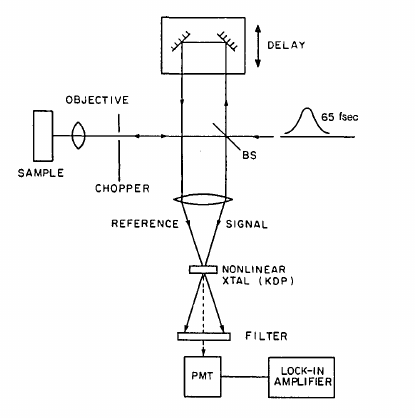
\includegraphics[width=0.45\linewidth]{gfx/ch2/fujimoto-setup}} \quad
	\subfloat[Lettuce leaf]
	{\label{fig:fujimoto-rabbit}
		\includegraphics[width=0.45\linewidth]{gfx/ch2/fujimoto-rabbit}}\\
	\caption{ Optical ranging setup (left) and measurement (right) of the cornea of the rabbit eye \cite{Fujimoto1986}. }\label{fig:fujimoto}
\end{figure}

This imaging technique is also called \emph{Optical Ranging}, and was demonstrated by \citeauthor{Fujimoto1986}\cite{Fujimoto1986} in 1986. An A-scan of the cornea of a rabbit's eye was performed \emph{in vivo}, and is available in \autoref{fig:fujimoto-rabbit}. The peaks in signal intensity located at $l = 0$ and $l \sim 450$ $\mu$m are due to the strong reflection occurring at the interface between two different media. Inbetween these two peaks it's also possible to notice the effect of light scattered by the cornea, which is not present in the air and aqueous regions. 


To acquire B-scans and C-scans, axial measurements can be repeatedly performed while moving the sample on the orthogonal plane or by deflecting the impinging optical beam by means of galvanometric mirrors. 

The main disadvantage of this scheme is the slow acquisition rate, as it requires the mechanical movement of the reference arm. Consequently, \emph{in vivo} imaging is difficult to achieve since the movement of the sample could introduce heavy distortions on both B-scans and C-scans. 

\section{Fourier Domain OCT}
\label{sec:fdoct}
\acf{FD-OCT} is a group of OCT techniques that encode the depth information of a sample in the frequency content of the interference signal and decode it through a Fourier trasform operation. As opposed to \ac{TD-OCT}, an axial scan is obtained without the need of a scanning mirror in the reference arm. This results in a much faster acquisition speed and higher quality measurements, since the distortions caused by the mechanical vibrations and uncertainty on the position of the mirror are removed. On the other hand, \ac{FD-OCT} systems require more advanced laser sources and detection schemes, other than some numerical compensation and high speed \acp{ADC}. 


The two main \ac{FD-OCT} schemes are called \acf{SD-OCT} and \acf{SS-OCT}, and will be presented in the next sections. 

\begin{figure}[hbt]
	\myfloatalign
	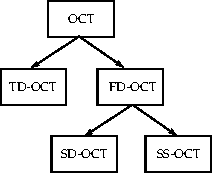
\includegraphics[width=0.5\linewidth]{gfx/ch2/oct-modalities}
	\caption{Diagram illustrating the different types of OCT modalities.}\label{fig:oct-modalities}
\end{figure}

\begin{figure}[hbt]
	\myfloatalign
	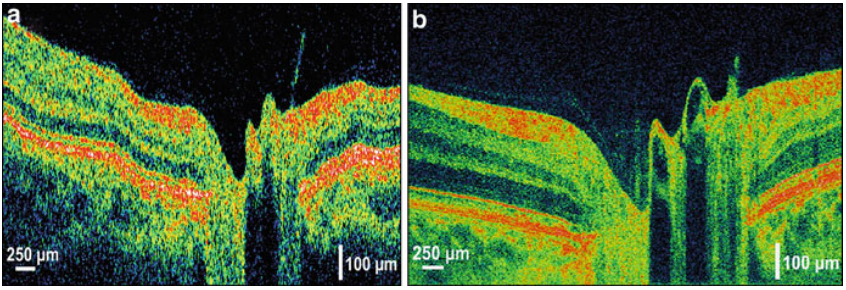
\includegraphics[width=0.95\linewidth]{gfx/ch2/td-fd-comparison}
	\caption{Comparison between images of the human retina obtained with standard \ac{TD-OCT} (left) and high-speed, high-resolution \ac{FD-OCT} (right).}\label{fig:td-fd-comparison}
\end{figure}

\subsection{Spectral Domain OCT}
\ac{SD-OCT} was the first type of \ac{FD-OCT} to be implemented, and was proposed by \citeauthor{Wojtkowski2002} in 2002 \cite{Wojtkowski2002}. This technique uses a \ac{SLD} as a broadband optical source, a Michelson interferometer similar to that in \autoref{fig:tdoct-michelson} and a detector consisting of a spectrometer. A diagram of the setup is available in \autoref{fig:fdoct-setup}. As already mentioned in \autoref{sec:fdoct}, \ac{SD-OCT} can acquire an A-scan with a single optical pulse, without the need to select the imaging depth through a scanning reference mirror. This comes at the price of a more complex detection scheme and the need for computationally intensive post-processing solutions. In order to achieve real-time performances, \ac{SD-OCT} schemes typically require the use of fast \acp{GPU}. 

\begin{figure}[hbt]
	\myfloatalign
	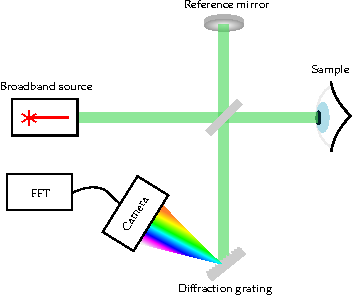
\includegraphics[width=0.75\linewidth]{gfx/ch2/fdoct-setup}
	\caption{Diagram of a typical \ac{SD-OCT} scheme.}\label{fig:fdoct-setup}
\end{figure}


To gain insight on the working principle of \ac{SD-OCT}, we can rewrite \autoref{eq:tdoct-interference} as a function of the wavenumber $k = 2\pi/\lambda$ and fixing the \ac{OPD}:
\begin{equation}
	I(k) \propto I_{source}(k)\cos\left(k \Delta z\right)
\end{equation}
This means that a reflector placed at a depth $d = \Delta z/2$ will frequency modulate the source spectrum with a frequency that is linearly dependant on $d$. This effect is illustrated in \autoref{fig:fdoct-spectrum} for a broadband source centered at 1310 nanometers, with ideal reflectors positioned at $d_1 = \Delta z/2 = 12.5$ $\mu$m and $d_2 = \Delta z/2 = 25$ $\mu$m. 

\begin{figure}[hbt]
	\myfloatalign
	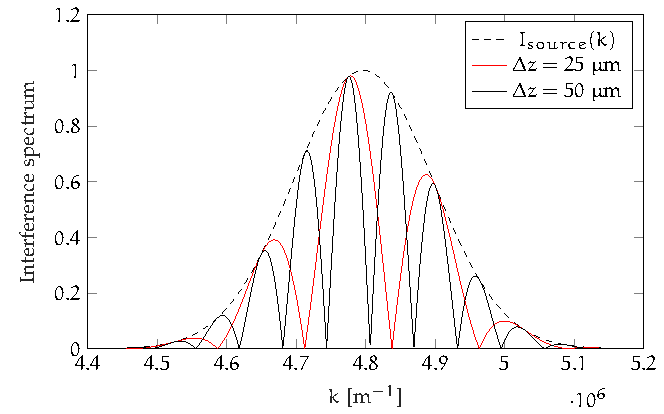
\includegraphics[width=0.85\linewidth]{gfx/tikz/fdoct-spectrum}
	\caption{\ac{SD-OCT} interference spectrum generated by two reflective surfaces.}\label{fig:fdoct-spectrum}
\end{figure}

Using a diffraction grating or a prism, the spectrum of the interference signal is spatially separated and acquired through a linear photodetector, typically a \ac{CCD} or \ac{CMOS} camera. The corresponding A-scan is then computed using an inverse Fourier Transform operation, mapping modulation frequency to axial position. The depth of the various layers of the sample are encoded in the modulation frequency of the spectrum, while their reflectivity is encoded in the fringe visibility. 

A key observation has to be made regarding the role of the coherence function $\gamma$. In fact, the spectrum modulation induced by a reflection at depth $d=\Delta z /2$ can only be detected if $\gamma(d/2)$ is non-zero, that is, only the portion of the sample that is within the coherence length of the source can be imaged. This is the main disadvantage compared to \ac{TD-OCT} schemes, in which the depth of focus in the sample was selected with the mechanical movement of the reference mirror.


\subsubsection{Drawbacks}

\paragraph{Sampling distortion}
One of the major problems corcerning this detection technique is that the interference spectrum is usually detected linearly in the wavelength domain. For example, a diffraction grating spatially separates the different wavelengths at an angle $\beta_m$ with respect to the axis normal to the grating such that
\begin{equation}
	\sin\beta_m = m \frac{\lambda}{\Lambda} + \sin\alpha,
\end{equation}
where $\Lambda$ is the spacing between each line of the grating, $\alpha$ is the angle of the inpinging wave and $m$ is the order of diffraction. 
This behaviour requires a re-sampling of the acquired spectrum before computing the Fourier Transform in order to obtain a signal which is linearly spaced in frequency instead of wavelength. If this post-processing step is ignored, an oscillating term with a fixed frequency $\propto \Delta z$ in the interference spectrum will result in a broadened peak in the Fourier domain, as can be observed in \autoref{fig:fdoct-resampling}. The linear sampling in the $\lambda$ domain will induce a chirp on the spectrum (red). Such behaviour has a detrimental effect on the axial resolution of the system. 


\begin{figure}[hbt]
	\myfloatalign
	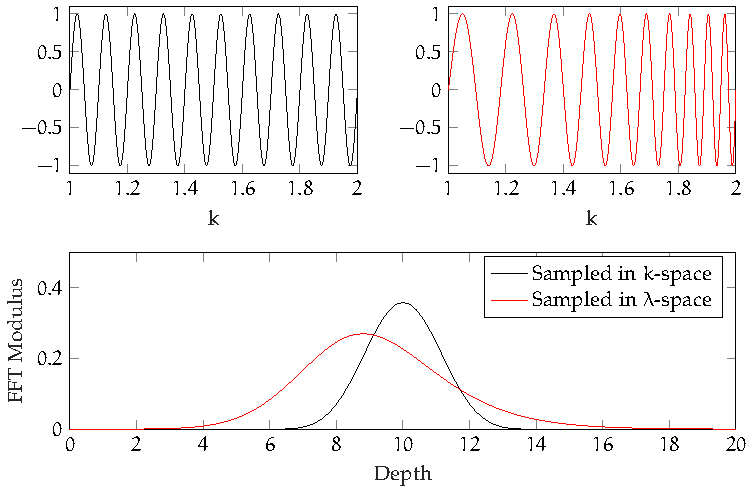
\includegraphics[width=0.95\linewidth]{gfx/tikz/fdoct-resampling}
	\caption{Interference distortion induced by linear sampling in the $\lambda$ space. }\label{fig:fdoct-resampling}
\end{figure}

\paragraph{Sensitity falloff}
A second harmful effect on the performance of this type of FD-OCT devices is the so-called \emph{Sensitivity falloff}. Sensitivity is defined as the \ac{SNR} when the sample is an ideal reflector. It's been experimentally demostrated that for increasing imaging depths, the sensitivity value drops. Such effect is illustrated in \autoref{fig:falloff}. This behaviour is due to the fact that when increasing the \ac{OPD} between reference and sample arm, the coherence function $\gamma(\Delta z)$ decreases as the two reflected signals only partially overlap, resulting in a lower signal intensity. 

\begin{figure}[bth]
	\myfloatalign
	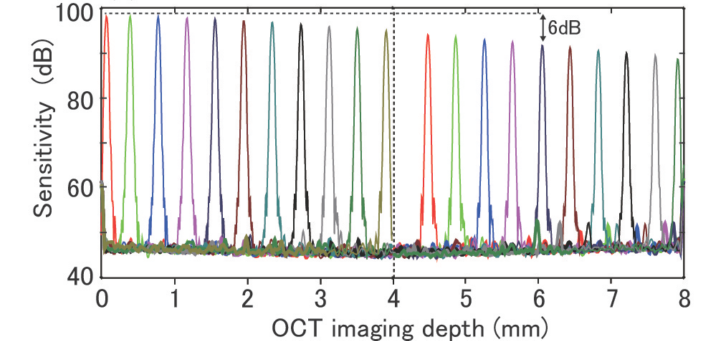
\includegraphics[width=\linewidth]{gfx/ch2/falloff}
	\caption{Sensitivity falloff in \ac{FD-OCT} systems \cite{Choi2012}.}\label{fig:falloff}
\end{figure}


An additional factor that contributes to this detrimental effect is the resolution of the photodetector arrays used to acquire the interference signal. As previously explained, higher imaging depths correspond to higher spectrum modulation frequencies. If the number of pixel $N$ of, e.g., a \ac{CCD} camera is not sufficiently high, the higher frequency components will be undersampled, reducing the range of visibility. Beam diameter and camera's pixel size also influence the loss of sensitivity. 

\paragraph{Imaging Artifacts} The massive gain in acquisition rate that comes from detecting the whole imaging range in a single shot is offset by the introduction of different artifacts in the reconstructed A-scans. The interference pattern acquired by the photodetectors array comprises three terms:
\begin{enumerate}
	\item \emph{DC component}. All the reflected replicas of the impinging signal coming from the sample contribute to a constant DC offset in the interference signal. These are equivalent to the non-interfering terms in the Michelson interferometer formula. When Fourier-transformed, they will appear as a reflector positioned at the very start of the imaging range, where the \ac{OPD} is close to zero. A simple solution to this problem is to compute and subtract the average value of the spectrum before applying the Fourier Transform.
	
	\item \emph{Cross-Correlation terms}. These are the interference terms that arise from the correlation between the reference signal and the reflections coming from the sample arm. As previously discussed, they contain the information required to reconstruct the reflectivity profile of the sample. 
	
	\item \emph{Auto-Correlation terms}. They result from the interference between reflectors in the sample that are less than a coherence length apart. 
\end{enumerate}


\begin{figure}[hbt]
	\myfloatalign
	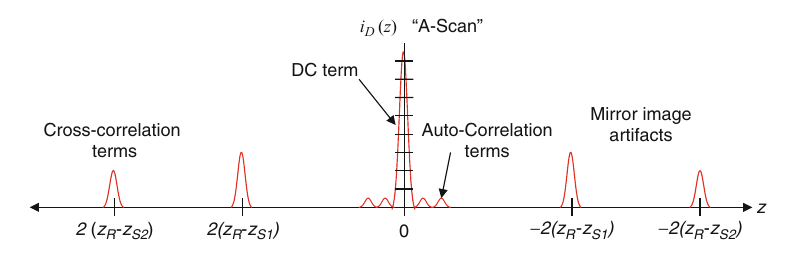
\includegraphics[width=\linewidth]{gfx/ch2/fdoct-artifacts}
	\caption{Artifacts contained in the \ac{FD-OCT} A-scans\cite{Drexler2015}}\label{fig:artifacts}
\end{figure}

These components are visible in \autoref{fig:artifacts}, who depicts the Fourier Transform of the interference signal generated by two reflectors. A further issue that is highlighted by this plot is the presence of the so called \emph{complex conjugate artifacts}, or mirror image artifacts. This phenomenon arises from the Fourier Transformation of a real signal, which will have the property of Hermitian simmetry (even magnitude and odd phase). This means that \ac{FD-OCT} techniques cannot differentiate between positive and negative frequencies, or equivalently, between a sample placed before or after the zero \ac{OPD} position. 

The easiest way to deal with this problem is to simply drop one half of the acquired A-scan, effectively halving the maximum imaging depth of the system. Mirror artifacts will still appear in the image if the sample is too close to the scanning lens and crosses the zero \ac{OPD} position, which is fixed by the reference mirror. The part of the sample which is in the "negative" \ac{OPD} range will appear flipped and superimposed to the other part of the sample. This effect is illustrated in \autoref{fig:artifacts-mirror}, in which the scanning lens is progressively moved forward, closer to the patient's retina. 

Different methods to solve this issue and restore the full imaging range have been proposed, including complex-signal detection schemes using 3x3 fiber couplers \cite{Sarunic2005}, heterodyne detection \cite{Davis2005} and phase-shifting techniques \cite{Tao2007} using either \acp{PZT} or \acp{EOM}. 

\begin{figure}[bth]
	\myfloatalign
	{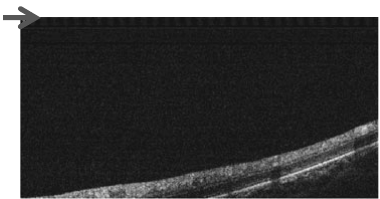
\includegraphics[width=.45\linewidth]{gfx/ch2/a}} \hspace{0.3cm}
    {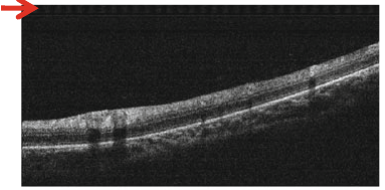
\includegraphics[width=.45\linewidth]{gfx/ch2/b}} \\[0.5cm]
	{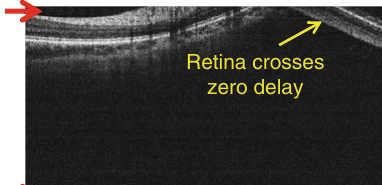
\includegraphics[width=.45\linewidth]{gfx/ch2/c}} \hspace{0.3cm}
	{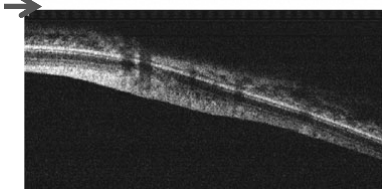
\includegraphics[width=.45\linewidth]{gfx/ch2/d}}
	\caption{Complex conjugate artifacts in \ac{SD-OCT}.}\label{fig:artifacts-mirror}
\end{figure}




\subsection{Swept-Source OCT}
\acf{SS-OCT}, also known as \ac{OFDI}, is a \ac{FD-OCT} technique that employs a narrow-bandwidth frequency-swept laser as an optical source. The introduction of tunable sources simplifies the detection scheme, removing the need for diffraction gratings and photodetector arrays. Ideally, a swept-source laser for \ac{SS-OCT} should present a frequency sweep that is linear, i.e, the istantaneous optical frequency should be expressed as
\begin{equation}\label{eq:frequency-sweep-linear}
	f(t) = f_0 + \sigma_f \cdot t,
\end{equation}
where $\sigma_f$, typically measured in Terahertz per microsecond, is the sweep speed of the source. If this requirement is satisfied, the intensity at the ouput of the interferometer when the sample is a single reflector positioned at the depth $d = \Delta z/2$, can be expressed as
\begin{equation}
	I(t) = I_1 + I_2 + 2\sqrt{I_1I_2}\cos\left( 2\pi \Delta f  t\right)\,
\end{equation}
where 
\begin{equation}
	\Delta f = \sigma_f \cdot \Delta t = \sigma_f \cdot \frac{\Delta z}{c} = \sigma_f \cdot \frac{d}{2c},
\end{equation}

 called the \emph{beat frequency}, is linearly dependant on the depth of the reflector. When the reflector is replaced by a real sample, multiple beat frequencies arise in the photodetector's current and the reflectivity profile can be reconstructed with a Fourier Transform. This technique is equivalent to \ac{SD-OCT}, with the key difference that the frequency sweep enables the detection as a function of time through a simple photodetector, while the diffraction grating spatially separates the different wavelengths and directs over a photodetector array.


\begin{figure}[hbt]
	\myfloatalign
	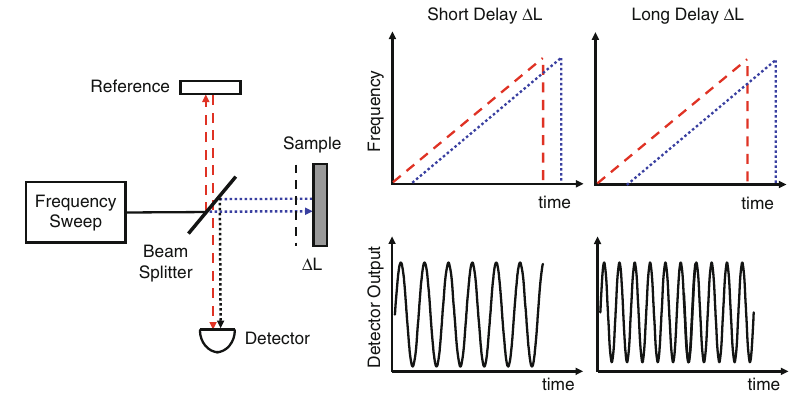
\includegraphics[width=\linewidth]{gfx/ch2/ssoct}
	\caption{Diagram of a typical SS-OCT scheme \cite{Drexler2015}}\label{fig:ssoct}
\end{figure}

\subsubsection{Sweep nonlinearity}
A tunable laser generally consists of a gain medium, typically a semiconductor optical amplifier (\acs{SOA}), a tunable wavelength filter and a laser cavity that supports a large bandwidth. The frequency-sweep is achieved by controlling the tunable filter through electrical signals to select the desired wavelength. \autoref{fig:sslaser} shows the diagram of an Axsun swept source in which frequency tuning is achieved by tilting a \ac{MEMS} mirror at the end of a Fabry-Perot filter. Rapidly changing the selected wavelength can affect the linearity frequency sweep, contributing to a nonlinear term in \autoref{eq:frequency-sweep-linear}, which then becomes

\begin{equation}
	f(t) = f_0 + \sigma_f \cdot t + \eta (t),
\end{equation}

where $\eta(t)$ contains the aforementioned nonlinearities. If the detector's output is digitized with a uniform clock rate, a similar effect to that described for \ac{SD-OCT} systems can arise (\autoref{fig:fdoct-resampling}), resulting in a non-linear sampling in the $k$-space. Consequently, distortions in the acquired A-scans can appear, hindering the image quality. A resampling of the acquired signal is then required in order to linearize the frequency sweep, adding to the total computational cost and possibly reducing the acquisition rate of the system. 


\begin{figure}[hbt]
	\myfloatalign
	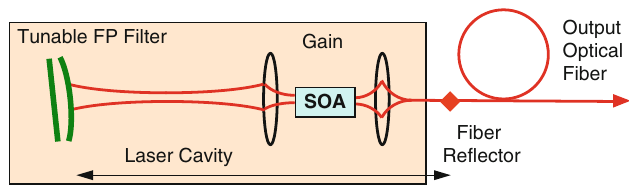
\includegraphics[width=0.7\linewidth]{gfx/ch2/sslaser}
	\caption{Frequency-swept optical source by Axsun \cite{Drexler2015}.}\label{fig:sslaser}
\end{figure}

\subsubsection{k-clocking}

While in \ac{SD-OCT} the resampling step is the only possible solution for this issue, \ac{SS-OCT} enables a hardware approach through a non-uniform clocking of the \ac{DAQ} device. This is accomplished by extracting a clock signal, called \emph{k-clock}, by means of an unbalanced \acf{MZI} which detects the frequency-sweep and generates a sinusoidal signal with a variable frequency. This approach removes the need for the computationally-intensive resampling step, but requires special \ac{DAQ} devices that can handle external clocks with a wide range of frequencies and duty cycles.  

\subsubsection{Acquisition rate}

The acquisition speed of \ac{SS-OCT} systems is dictated by the source sweep repetition rate, that is, the frequency at which the source is able to sweep the entire bandwidth. This parameter is determined by the laser cavity length. In fact, for a given frequency, the spontaneous emission has to build up in order to reach a saturation limit to be correctly amplified by the active region. Shorter cavities with a smaller round-trip generally guarantee higher repetition rates than longer cavities. Novel swept-source designs enable acquisition speeds in the order of 100,000 A-scans per second, with \ac{FDML} and \acp{VCSEL} reaching repetition rates above 500 kHz. These unprecedented values make \ac{SS-OCT} the primary candidate for real-time 3D visualization of \emph{in vivo} samples, where motion artifacts could hinder image quality. This is possible because the detection scheme is no longer the bottleneck like in \ac{SD-OCT}, where slow camera response times limited the overall rate of the system. 

\subsubsection{Axial resolution}
Just like in the case of \ac{SD-OCT}, the axial resolution depends on the tuning range of the source, $\Delta \lambda$, which is defined as the \ac{FWHM} of the spectrum. In the case of a Gaussian spectrum, the axial resolution, defined as the \ac{FWHM} of the reflection peak generated by a perfect reflector, is given by
\begin{equation}\label{eq:ss-axial-resolution}
	\delta z \simeq 0.75 \cdot \frac{\lambda_0^2}{\Delta \lambda},
\end{equation}
where $\lambda_0$ is the central wavelength of operation, which is chosen based on the application (1060 nm for Ophtalmology, 1300 nm for tissue imaging). 

\subsubsection{Imaging range}
Imaging range of \ac{SS-OCT} systems is, like other \ac{FD-OCT} schemes, limited by the coherence length of the source, which we have previously defined as the \ac{OPD} at which the visibility of the interference fringes drops to half of its maximum. This parameter is controlled by the istantaneous linewidth of the source $\delta \lambda$ by the following equation:
\begin{equation}
	l_c \approx 0.44 \frac{\lambda_0^2}{\delta \lambda}.
\end{equation}

As with \ac{SD-OCT}, complex conjugate artifacts typically limit the imaging range to be half of the coherence length. 

When using a $k$-clock to acquire A-scans, the imaging range is also dependant on the path difference of the \ac{MZI}'s arms, which has to be 4 times the maximum imaging depth, $d_{max}$. A factor of 2 is needed because a reflector positioned at $d_{max}$ will have \ac{OPD} equal to $\Delta z = 2d_{max}$ with respect to the reference mirror. The other factor of 2 is needed to satisfy Nyquist's criterion, so that the $k$-clock will have a maximum frequency that is 2 times the beat frequency generated by the reflector at $d_{max}$. 

\subsubsection{Balanced detection}
The use of simple photodetectors instead of more complex setups involving diffraction gratings and prisms allows for a dual balanced detection scheme. By collecting the reference and sample signals through a circulator and feeding them to a 3 dB fiber coupler, two interference signals can be obtained. A balanced detector can then subtract the common DC component and excess noise, while at the same time summing the interference term. This detection scheme has been proved to be more efficient than a simple Michelson interferometer. A complete \ac{SS-OCT} scheme with dual balanced detection and external $k$-clock is illustrated in \autoref{fig:ssoct-scheme}.

\begin{figure}[hbt]
	\myfloatalign
	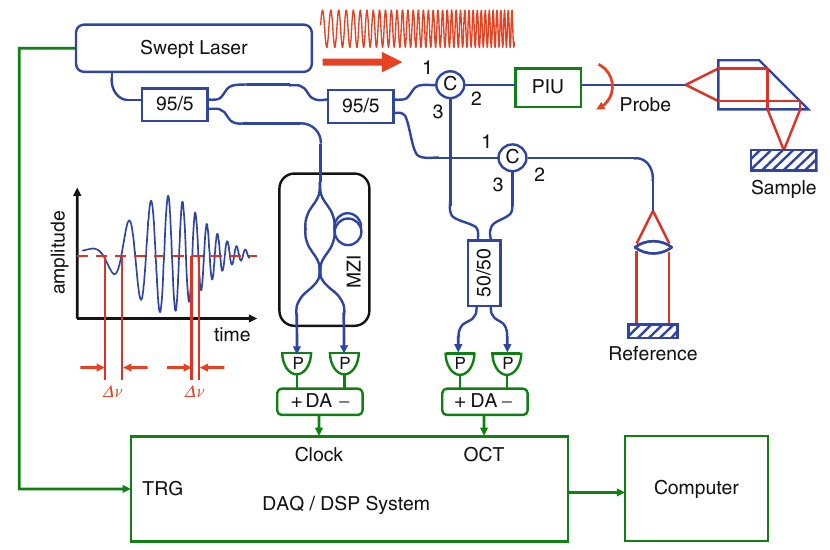
\includegraphics[width=\linewidth]{gfx/ch2/ssoct-scheme}
	\caption{Complete fiber optic SS-OCT scheme using an external clock source and balanced detection \cite{Drexler2015}.}\label{fig:ssoct-scheme}
\end{figure}

% Chapter 3

\chapter{Description of the Setup} % Chapter title
\label{ch:setup} % For referencing the chapter elsewhere, use \autoref{ch:mathtest}

This chapter details the setup that was used in the design of a Swept Source OCT system developed for this thesis work, describing the optical and electrical components that were employed. 

\noindent Particular care will be given to the characterization of the \ac{DAQ} board and the design of the acquisition software. 

\section{Optical Source}
As already discussed in \autoref{ch:theory}, \ac{SS-OCT} systems employ a narrow-bandwidth tunable laser to enable a simple detection scheme and is one of the most critical components of the entire system. The source that was used in this thesis is a SSOCT-1310 by Axsun Technologies, which is a class 3 laser that uses a \ac{MEMS} tunable filter to sweep wavelengths in the 1300 nm range. 

The two most important features of this laser are the fast sweep rate, which enables high speed imaging, and the presence of the $k$-clock signal used for equalizing the nonlinear frequency sweep. 

\begin{figure}[bth]
	\myfloatalign
	{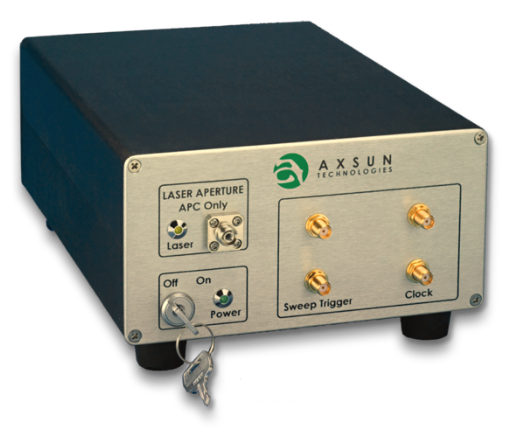
\includegraphics[width=.6\linewidth]{gfx/ch3/axsun}}
	\caption{The acquisition board, AlazarTech ATS9350.}\label{fig:axsun-laser}
\end{figure}

An photo of the laser is available in \autoref{fig:axsun-laser}. The emitted light is collected by connecting a fiber optic patch cord to the FC/APC connector on the front panel, which also includes two SMA connectors for the sweep-start trigger and the $k$-clock signal.


  \begin{table}
	\myfloatalign
	\begin{tabularx}{\textwidth}{Xll} \toprule
		\tableheadline{Parameter} & \tableheadline{Units} & \tableheadline{Value}
		\\ \midrule
		Sweep Rate &  kHz & 100.2 \\
		Center Wavelength & nm & 1305 \\
		Wavelength Tuning Range & nm & 140.38 \\
		Average Power & mW & 25.7 \\
		Duty Cycle & \% & 77.3 \\
		Sampled Duty Cycle & \% & 50.5 \\
		External Clock Min Frequency & MHz & 183.1 \\
		External Clock Average Frequency & MHz & 307.0 \\
		External Clock Max Frequency & MHz & 332.1 \\
		Sampling Clocks & -- & 1536 \\
		\bottomrule
	\end{tabularx}
	\caption{Axsun laser datasheet.}
	\label{tab:axsun-datasheet}
\end{table}

\subsection{Optical Spectrum}
A critical parameter in swept sources for OCT applications is the wavelength interval over which the laser is able to tune. From \autoref{tab:axsun-datasheet}, we can see that the Axsun SSOCT-1310 is centered at $\lambda_0 = 1305$ nm with a bandwidth of $\Delta\lambda = 140.38$ nm. These values were verified by connecting the laser output directly to an \ac{OSA}, measuring its spectrum. 

\begin{figure}[hbt]
	{\myfloatalign
		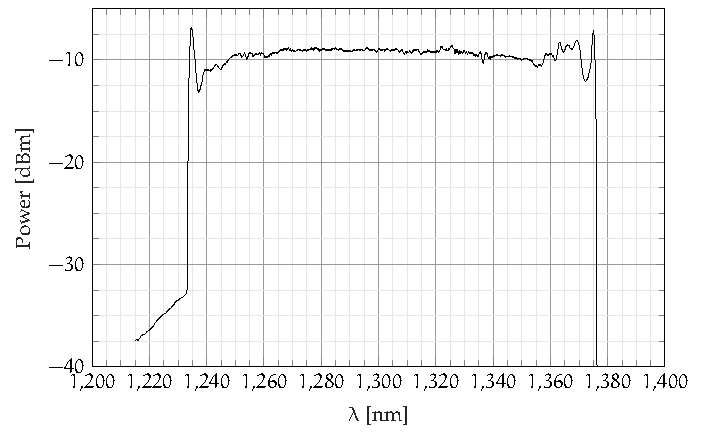
\includegraphics[width=\linewidth]{gfx/tikz/axsun/spectrum}}\\
	\caption{Spectrum of the Axsun SSOCT-1310 laser, obtained with a 1 nm resolution.}\label{fig:axsun-spectrum}
\end{figure}

The measurement was executed with a resolution of 1 nanometer, resulting in the spectrum visible in \autoref{fig:axsun-spectrum}. The edge wavelengths turned out to be $\lambda_1 \approx 1237$ nm and $\lambda_2\approx1376$ nm, which result in a bandwith of $\Delta \lambda \approx 139$ nm and central wavelength of $\lambda_0\approx 1307$ nm. These values slightly differ from those reported in the datasheet, but not enough to compromise the performance of the laser. 

The bandwidth is swept at a frequency $f_a = 100.2$ kHz and with a duty cycle $d_c=0.505$, meaning that the average sweep speed is 
\begin{equation}
\sigma_{\lambda} = \frac{\Delta\lambda f_c}{d_c} \approx 27.8 \,\,\text{nm}/\mu\text{s}.
\end{equation}

Since the goal of SS-OCT sources is to perform a linear frequency sweep, it is more useful to define this parameter in the following manner
\begin{equation}\label{eq:sweep-speed}
\sigma_f = c_0 \left(	\frac{1}{\lambda_0 - \Delta\lambda/2} - \frac{1}{\lambda_0 + \Delta\lambda/2}\right) \frac{f_a}{d_c} \approx 4.9 \,\,\text{THz}/\mu\text{s}
\end{equation}

The istantaneous frequency, after linearization, is thus expressed by 
\begin{equation}
	f(t) = f_0 + \sigma_f t
\end{equation}
where the starting frequency is determined by
\begin{equation}
f_0 = \frac{c_0}{\lambda_0 + \Delta\lambda /2} \approx 218.2 \,\,\text{THz}.
\end{equation}

\subsection{Axial Resolution}
Using \autoref{eq:ss-axial-resolution} and the data provided by \autoref{tab:axsun-datasheet} it is possible to obtain an estimate of the axial resolution provided by the employed optical source. The axial resolution is then
\begin{equation}
\delta z \simeq 0.75 \frac{\lambda_0^2}{\Delta \lambda} \approx 9.2 \,\, \mu\text{m.}
\end{equation}

This approximation is valid for sources with a Gaussian spectrum, and can lead to an overestimation of the real axial resolution of the system in case this condition is not met. 

\subsection{Sweep trigger}
The Axsun laser provides a square-wave signal that determines the start of the frequency sweep  and that is used to trigger the acquisition of A-scans. This signal is acquired with a high-speed oscilloscope and illustrated in \autoref{fig:axsun-trigger}. The voltage range was measured as $V_{range} \approx [0 ,1.48] $ V, while the duty cycle is found to be 
\begin{equation}
	d_c = \frac{t_{high}}{t_{high} + t_{low}} \approx 0.97\,.
\end{equation}

For a correct acquisition of A-scans, the datasheet recommends to trigger the acquisition device when the signal level reaches the value of $V_{trig} = 0.71$ V, pictured in \autoref{fig:axsun-trigger} with a red line. 


\begin{figure}[hbt]
	\myfloatalign
	{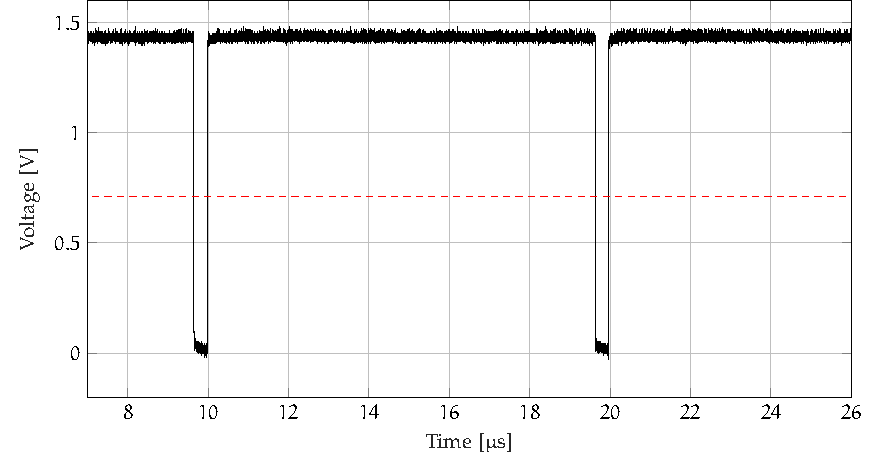
\includegraphics[width=0.8\linewidth]{gfx/ch3/trigger}}\\
	\caption{Sweep trigger of the SSOCT-1310 laser.}\label{fig:axsun-trigger}
\end{figure}

\subsection{Power profile}
Using a photodiode it's possible to measure the istantaneous power profile of the laser emission. The photodiode generates an electrical current which is proportional to the power of the detected electromagnetic field: 
\begin{equation}
	I_{ph} = \mathcal{R} \cdot P 
\end{equation}
The constant $\mathcal{R}$ is called \emph{responsivity} [A/W] and is specific to the detector used. The current can then be measured with an oscilloscope. In order to avoid the saturation of the receiver, a 3 dB coupler was inserted between the source and the photodiode. The obtained power profile is depicted in \autoref{fig:axsun-power} along with the sweep trigger. We can observe that in the first $\sim 5$ $\mu$s after the positive edge of the trigger, the istantaneous power behaves like a typical laser pulse while outside of this interval it assumes an irregular profile. 


\begin{figure}[hbt]
	\myfloatalign
	{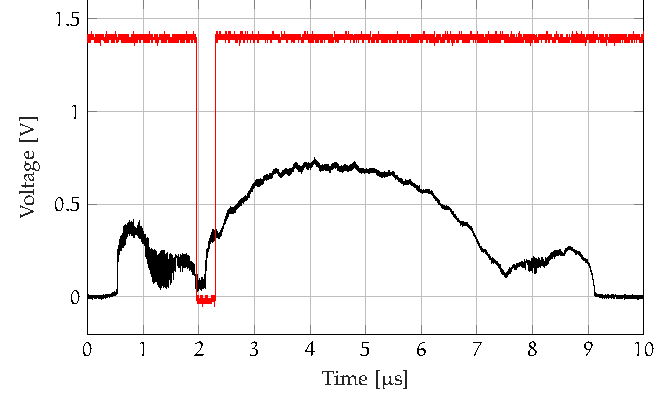
\includegraphics[width=0.8\linewidth]{gfx/ch3/power-profile}}\\
	\caption{Sweep trigger of the SSOCT-1310 laser.}\label{fig:axsun-power}
\end{figure}


\subsection{k-clock}
As already stated, this particular SS-OCT laser is equipped with an internal \ac{MZI} which generates the variable-frequency clock, called $k$-clock, used to sample the A-scan signal at a variable rate and equalize the nonlinear terms in the frequency sweep. As we can see in \autoref{fig:kclock}, this signal assumes values in the $[0, 900]$ mV range with an average value of about 460 mV. This sinusoidal signal will be used to drive the acquisition board for the first $5$ $\mu$seconds of the sweep and from this point forward will be referred to as \emph{useful clock}. As per \autoref{tab:axsun-datasheet}, the total number of samples that cab be acquired using this clock is $N_s = 1536$. In the last 5 $\mu$seconds the clock is called "dummy" because of its undefined behaviour that could lead to issues in the clocking of the DAQ devices.

\begin{figure}[hbt]
	\myfloatalign
	{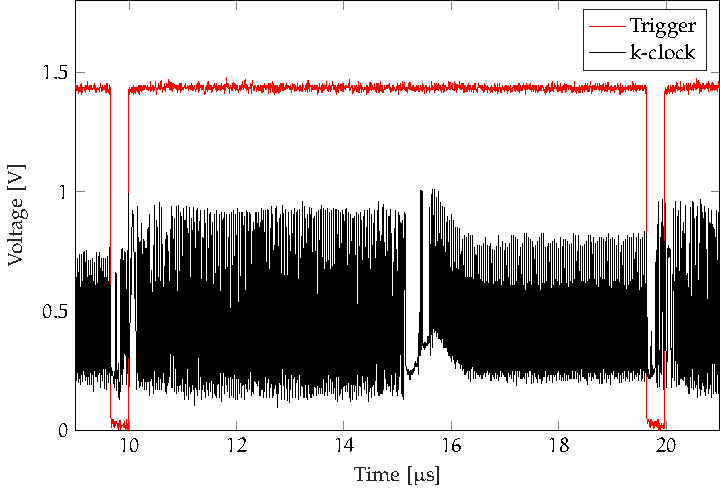
\includegraphics[width=0.8\linewidth]{gfx/ch3/clock}}\\
	\caption{Estimate of the istantaneous frequency of the k-clock.}\label{fig:kclock}
\end{figure}

In \autoref{fig:clock-zoom} are depicted two 50 nanoseconds windows at the start (left) and in the middle (right) of the useful clock, where the variable frequency of signal is clearly visible. Also worth noting is that at the start of the sweep the signal appears much more distorted than in the middle of the sweep. Fortunately, this behaviour did not compromise the performance of the system. 

\begin{figure}[bth]
	\myfloatalign
	{\includegraphics[width=.45\linewidth]{gfx/ch3/clock1}} \quad
	{\includegraphics[width=.45\linewidth]{gfx/ch3/clock2}} \\
	\caption{Behaviour of the useful k-clock at different time instants.}\label{fig:clock-zoom}
\end{figure}

To gain further insights on the nature of the frequency sweep, it is interesting to estimate the istantaneous frequency of the k-clock. A method to perform this estimate is the following
\begin{enumerate}
	\item Subtract the average value from the signal
	\item Interpolate the signal $(t, y)$ to obtain $(\hat{t}, \hat{y})$
	\item Determine the time instants $\hat{t}_i$ at which the signal $\hat{y}$ crosses 0, from which a vector $\mathcal{I} = \left[\hat{t}_{i_1}, \hat{t}_{i_2}, \dots,  \hat{t}_{i_N}\right]$ is built.
	\item Compute the difference between the adjacent elements of $\mathcal{I}$ and obtain $\mathcal{T} = \left[\hat{\tau}_{i_1}, \hat{\tau}_{i_2}, \dots,  \hat{\tau}_{i_{N-1}}\right]$,
	\item The istantaneous frequency of the signal is then estimated as $\hat{f}_i = 1/2 \hat{\tau}_i$.
\end{enumerate} 

The result of this method is illustrated in \autoref{fig:kclock-frequency}. Since the estimate is rather noisy, a low pass filter was applied to the $\hat{f}_i$ signal, resulting in a much cleaner estimation (depicted in red). As we can observe, the istantaneous frequency rapidly changes at the start and at the end of the sweep, while in the middle it stabilizes at about 320 MHz. Since a constant k-clock frequency implies a linear frequency sweep, we can infer that the sweep nonlinearities are much more prevalent at the edge of the sampling interval. 

The maximum estimated frequency is $\hat{f}_{clk}^{max} = 339$ MHz, as opposed to the value that was reported in \autoref{tab:axsun-datasheet} of $f_{clk}^{max} = 332.2$ MHz. This slight overestimation is also visible in \autoref{fig:kclock-frequency}, where we can see that the low-pass filtered signal is slightly higher than the average value of the non filtered one.

\begin{figure}[hbt]
	\myfloatalign
	{\includegraphics[width=0.8\linewidth]{gfx/ch3/lowpass}}\\
	\caption{Estimate of the istantaneous frequency of the k-clock.}\label{fig:kclock-frequency}
\end{figure}

From the maximum frequency of the k-clock signal we can measure the maximum imaging depth obtainable by the system. 

Two replicas of the pulse overlapping with a relative time delay $\tau$ will generate a beat frequency $f_b$ given by

	\begin{equation}
		f_b = \sigma_f \tau
	\end{equation}
	
where $\sigma_f$, the sweep speed, was determined in \autoref{eq:sweep-speed}. In a OCT setup, the time delay $\tau$ is related to the path mismatch of reference and sample arm, which in turn depends on the depth of the layer of the sample that generates the reflection. In this way	
	\begin{equation}
		\tau = \frac{2dn}{c_0},
	\end{equation}
where $c_0$ is the speed of light in vacuum, $n$ is the refractive index of the sample and $d$ is the depth. By the Nyquist theorem, the maximum beat frequency that can be digitized using the $k$-clock is
	
	\begin{equation}
		f_b^{max} = \frac{f_{clk}^{max}}{2},
	\end{equation}
which results in a maximum depth in air ($n=1$) of  
	\begin{equation}
		d_{max} = \frac{c_0 f_{b}^{max}}{2\sigma_f}  =  \frac{c_0 f_{clk}^{max}}{4\sigma_f} \simeq 5.1 \text{ mm}.
	\end{equation}

\subsection{Coherence length}
In \autoref{ch:theory} we have seen that the coherence length of a source is one of the most important parameters of optical sources, independently of the type of OCT system. In \ac{TD-OCT}, this parameter determines the axial resolution of the system, while \ac{FD-OCT} schemes it also affects the imaging range, as the reference arm is fixed. In particular, complex conjugate artifacts arising from the Fourier trasform of the detected signals halve the maximum imaging range. For this reason, the coherence length of a swept source satisfies the following inequality
\begin{equation}
	l_c \geq 2 \cdot d_{max},
\end{equation}
which implies that the coherence length of the SSOCT-1310 source is at least
\begin{equation}
	l_c \geq 2\cdot d_{max} \approx 10.2 \text{ mm.}
\end{equation}

The exact value was experimentally determined in \cite{Calabrese2017}, measuring the normalized coherence function $|\gamma(\Delta z)|$ by placing a mirror in the sample arm and acquiring the interference signal for different values of \ac{OPD}. The path length difference was changed by translating the reference mirror. The intensity of the interference signal, normalized by its maximum value, is plotted in  \autoref{fig:axsun-coherence-length} as a function of the \ac{OPD}. When the \ac{OPD} increases above a certain value, the coherence function decays exponentially as
\begin{equation}
|\gamma(\Delta z)| \propto e^{-\alpha |\Delta z|},
\end{equation}
which corresponds to a linear decay in the logarithmic domain. The parameter $\alpha$ was estimated by fitting the data points to a line using a Least-Squares fit. The coherence length is finally determined as the $\Delta z$ value such that $|\gamma(\Delta z)| = 1/2$, resulting in
\begin{equation}
	l_c = 2 \cdot \frac{\ln 2}{\alpha} \approx 12.3 \text{ mm.}
\end{equation}


\begin{figure}[hbt]
	\myfloatalign
	{\includegraphics[width=0.8\linewidth]{gfx/ch3/axsun-coherence-length}}\\
	\caption{Experimental estimation of the normalized coherence function.}\label{fig:axsun-coherence-length}
\end{figure}

\section{Scanning System}
One of the most critical components of an OCT is the scanning system. Its role is to receive the light emitted by the source, focus it on the sample under test, and collect the backreflections. A scanning system usually comprises of three different devices

\begin{enumerate}
	\item Fiber collimator
	\item Galvanometric Mirrors
	\item Focusing lens
\end{enumerate}

\begin{figure}[bth]
	\myfloatalign
	{\includegraphics[width=0.8\linewidth]{gfx/setup-diagrams/scanning-diagram.pdf}}
	\caption{Diagram of a OCT scanning system.}\label{fig:scanning-diagram}
\end{figure}

A schematic of this system is depicted in \autoref{fig:scanning-diagram}. Light coming from a single mode optical fiber is deflected by a system of galvanometric mirrors towards a lens which in turns focuses the radiation on the sample. By rotating the mirrors the light beam is focused on a different position on the sample. The reflected beam travels the same path in the opposite direction and is collected by the optical fiber. The correct design of these components is paramount in order to guarantee small transversal and axial resolutions of the OCT system. 



\subsection{Collimator}
The role of the fiber collimator is to collect light coming from a single mode fiber and collimate the beam on the galvanometric mirrors. The divergence angle at the output of the collimator is approximated with the following equation when the beams have a Gaussian intensity profile:
\begin{equation}
	\theta \approx \frac{D}{f} \frac{180}{\pi},
\end{equation}
where $D$ is the mode diameter and $f$ is the focal length of the collimator. This approximation works well for sigle mode fibers, but will underestimate the real divergence angle in the case of multimode fibers, as the intensity profile has a non-Gaussian shape. 

The collimator used in this setup is the Thorlabs F280APC-C\footnote{\url{https://www.thorlabs.com/thorproduct.cfm?partnumber=F280APC-C}}, which is designed to work in the 1310 nm range. Its main specifications are summarized in \autoref{tab:collimator-datasheet}. 

\begin{table}[h]
	\myfloatalign
	\begin{tabularx}{\textwidth}{Xll} \toprule
		\tableheadline{Parameter} & \tableheadline{Units} & \tableheadline{Value}
		\\ \midrule
		Central wavelength & nm & 1310 \\
		Beam diameter & mm & 3.4 \\
		Divergence angle & degrees & 0.028 \\
		Lens numerical aperture (NA) & -- & 0.15 \\
		Focal length & mm & 18.67 \\
		\bottomrule
	\end{tabularx}
	\caption{Thorlabs F280APC-C datasheet.}
	\label{tab:collimator-datasheet}
\end{table}

\subsection{Scanning lens}
The light beam deviated by the galvanometric mirrors has to be focused on the sample under test in order to guarantee high resolution images. This is accomplished by a telecentric focusing lens. This type of lenses is characterized by flat image planes which are ideal for OCT applications. 

The main parameters that characterize this device are the following:
\begin{itemize}
	\item Entrance Pupil Size (EP): it specifies the diameter of the collimated laser beam that will maximize the resolution of the imaging system. When using a single galvanometric mirror, the EP is located at the pivot point of the mirror. When two mirrors are used, the EP is located between the two mirrors. 

	\item Scanning Distance (SD): the distance between the EP and the base of the lens. 
	
	\item Scan Angle (SA): the angle between the incoming light beam and the optical axis of the lens. 
	
	\item Working Distance (WD): the distance between the tip of the lens and the focal plane.
	
	\item Parfocal Distance (PD): the distance between the base of the lens and the focal plane. It is equal to the WD plus the objective length.
	
	\item Field of View (FOV): the area on the focal plane that can be imaged with a resolution equal or better than the one guaranteed by the lens. 
	
	\item Depth of View (DOV): it corresponds to the distance between parallel planes on either side of the focal plane, where the beam spot diameter is $\sqrt{2}$ greater than it is at the focal plane. Using lenses with a high DOV value yields images with high lateral resolution in a larger interval of depths. 
	
	\item Spot size: the diameter of the beam on the focal plane. 
\end{itemize}


 The lens used for the SS-OCT system developed in this thesis is the Thorlabs LSM04\footnote{\url{https://www.thorlabs.com/thorproduct.cfm?partnumber=LSM04}}. Its main specifications are listed in \autoref{tab:lens-datasheet}. A simulation of the beam spot size on the focal plane is available in \autoref{fig:spotsize}, where we can see that it increases for bigger scan angles. This behaviour has the effect of reducing the lateral resolution at the edge of the FOV. 
 
\begin{figure}[bth]
 	\myfloatalign
 	{\includegraphics[width=0.6\linewidth]{gfx/ch3/spotsize}}
 	\caption{The Thorlabs GVS002 galvo system.}\label{fig:spotsize}
 \end{figure}
 
 
 
 \begin{table}[h]
 	\myfloatalign
 	\begin{tabularx}{\textwidth}{Xll} \toprule
 		\tableheadline{Parameter} & \tableheadline{Units} & \tableheadline{Value}
 		\\ \midrule
 		Wavelength range & nm & 1250-1380\\
 		Effective Focal Length (EFL) & mm & 54 \\
 		Entrance Pupil size & mm & 4 \\
 		Working Distance & mm & 42.3 \\		
 		Parfocal Distance & mm & 80.8 \\
 		Scan Distance & mm & 18.9 \\
 		Maximum Scan Angle & degrees & $\pm 7.5 \times \pm 7.5$ \\
 		Field of View & mm$^2$ & $14.1 \times 14.1$ \\
 		Depth of View & mm & 0.61\\
 		\bottomrule
 	\end{tabularx}
 	\caption{Thorlabs LSM04 datasheet.}
 	\label{tab:lens-datasheet}
 \end{table}
 
 
 
 \subsubsection{Lateral resolution}
 
 Using the parameters listed in \autoref{tab:lens-datasheet} it is also possible to obtain an estimate of the lateral resolution of the system, which is dictated by the diffraction limited spot size of the focused optical beam. For Gaussian-shaped beams, it is approximated as \cite{Drexler2015}
 \begin{equation}
 	\delta x \simeq \frac{4\lambda_0}{\pi} \frac{f}{d}
 \end{equation}
 where $\lambda_0$ is the central wavelength of operation, $f$ is the focal length of the focusing lens and $d$ is the diameter of the beam at the entrance of the lens. The lateral resolution guaranteed by the LSM04 lens is thus
 \begin{equation}
 	\delta x \simeq \frac{4\lambda_0}{\pi} \frac{EFL}{EP} \approx 22.5 \,\,\mu\text{m.}
 \end{equation}
 
 Since the diameter of the beam exiting the fiber collimator is slightly smaller ($d=3.4$ mm) than the EP size, the resulting lateral resolution becomes
 \begin{equation}
	\delta x \approx 26.5 \,\,\mu\text{m}.
 \end{equation}
 
 The depth of view, also called confocal parameter, limits the imaging depth of the system. Due to diffraction, this paramer is also governed by the lateral resolution of the system through the following equation
 \begin{equation}
	 b = \frac{2 \delta x^2}{\lambda_0}.
 \end{equation}
 
 This effect is illustrated in \autoref{fig:na}, where we can observe that using lenses with a high numerical aperture (NA), or small spot size, the depth of view is limited. In OCT systems it is preferred to use low NA lenses to sacrifice lateral resolution in favor of a depth of view comparable to the coherence length of the source. Following this criterion the coherence length is fully exploited. 
 
  \begin{figure}[bth]
 	\myfloatalign
 	{\includegraphics[width=0.6\linewidth]{gfx/ch3/na}}
 	\caption{Basic diagram of a  SS-OCT setup}\label{fig:na}
 \end{figure}
 
 
 Using the EP size the confocal parameter is $b \approx 0.61$ mm, equal to the value reported in \autoref{tab:lens-datasheet}, while using the beam size diameter $d = 3.4$ mm it becomes $b \approx 0.84$ mm. 
 
 

\subsection{Galvanometric Mirrors}

\begin{figure}[bth]
	\myfloatalign
	{\includegraphics[width=0.6\linewidth]{gfx/ch3/galvo}}
	\caption{The Thorlabs GVS002 galvo system.}\label{fig:galvo}
\end{figure}

\begin{figure}[bth]
	\myfloatalign
	{\includegraphics[width=0.75\linewidth]{gfx/ch3/galvo-distortion}}
	\caption{Field distortion using two mirrors.}\label{fig:galvo-distortion}
\end{figure}


\begin{figure}[bth]
	\myfloatalign
	{\includegraphics[width=0.75\linewidth]{gfx/ch3/testa}}
	\caption{Field distortion using two mirrors.}\label{fig:testa}
\end{figure}
	
\section{Acquisition Board}

    \begin{figure}[bth]
    \myfloatalign
    {\includegraphics[width=.6\linewidth]{gfx/board}}
    \caption{The acquisition board, AlazarTech ATS9350.}\label{fig:acq-board}
    \end{figure}
	\subsection{}

    \begin{figure}[bth]
    \myfloatalign
    \subfloat[Acquisition using Single-Port Memory.]
    {\label{fig:single-port-acq}
    \includegraphics[width=.75\linewidth]{gfx/single-port-acq}} \\
    \subfloat[Acquisition using Dual-Port Memory.]
    {\label{fig:dual-port-acq}
    \includegraphics[width=.75\linewidth]{gfx/dual-port-acq}}
    \caption{Diagram highlighting the differences between Sigle-Port acqusitions and Dual-Port acqusitions}\label{fig:single-vs-dual-port}
    \end{figure}

    In \autoref{fig:single-vs-dual-port} a comparison between the two acquisition techniques is available. For Single-port Acquisitions, in \autoref{fig:dual-port-acq} we can see that no trigger events are missed and over 95\% of CPU time is available for data processing, while in \autoref{fig:single-port-acq} trigger events happening while the DMA transfer is ongoing are missed completely, and virtually all CPU cycles are used in managing the data acquisition. This leaves no room for data processing on the CPU. 
    


\section{Optical Circuit}

\subsection{ Mach-Zender Interferometer }
In order to test the k-clock and the acquisition device blah blah blah used AlazarDSO softeare to obtani the beating signal of unbalanced MZI -> show difference also on images
\begin{figure}[bth]
	\myfloatalign
	{\includegraphics[width=\linewidth]{gfx/setup-diagrams/interferometer.pdf}}
	\caption{Diagram of an unbalanced Mach-Zender Interferometer.}\label{fig:unbalanced-mzi}
\end{figure}

\subsection{Basic setup and Stability Analysis}


\subsection{Final Setup with OBR balancing}
Add couplers length measurements;  focus in the middle of the imaging range. 

\subsection{Axial Resolution}
Try with new measurements

\subsection{Thickness measurements}
No scattering detected, only reflections caused by the surface


\begin{figure}[hbt]
\myfloatalign
{\includegraphics[width=\linewidth]{gfx/falloff}}
\caption{Signal spectrum at various depths.}\label{fig:power-falloff}
\end{figure}


\begin{figure}[hbt]
\myfloatalign
{\includegraphics[width=0.9\linewidth]{gfx/falloff-fit}}
\caption{Signal-to-noise ratio falloff.}\label{fig:falloff-fit}
\end{figure}



\begin{figure}[hbt]
\centering
\includegraphics[width=\linewidth]{gfx/tikz/axsun/banana-peel}
\caption{B-scan of banana peel.}\label{fig:banana-peel}
\end{figure}%----------------------------------------------------------------------------------------
\begin{figure}[hbt]
\myfloatalign
{\includegraphics[width=\linewidth]{gfx/tikz/axsun/dry-orange-peel}}
\caption{B-scan of dry orange peel.}\label{fig:dry-orange-peel}
\end{figure}%----------------------------------------------------------------------------------------

\begin{figure}[hbt]
\myfloatalign
{\includegraphics[width=\linewidth]{gfx/tikz/axsun/finger}}
\caption{B-scan of a human finger.}\label{fig:finger}
\end{figure}%----------------------------------------------------------------------------------------
%----------------------------------------------------------------------------------------

% Chapter X

\chapter{Results} % Chapter title
\label{ch:results} % For referencing the chapter elsewhere, use \autoref{ch:name} 

This chapter is dedicated to the description of the OCT software that was developed for this thesis. This application handles the data acquisition task, controls the galvanometric system and performs real-time processing and visualization of the acquired OCT data. \\

\noindent The transversal resolution of the system described in \autoref{ch:setup} is also evaluated using the test resolution target introduced in the same chapter. \\

\noindent Finally, a series of B-scans, C-scans and \emph{en-face} images of a variety of different samples is presented. A part of these were acquired using a second SS-OCT system designed to work in the 1060 nm range. 


%----------------------------------------------------------------------------------------

\section{Data Acquisition Software}

The final component that is needed to obtain a working SS-OCT system is a computer application that handles data acquisition and image visualization. This program should be able to achieve real-time performances, enabling a low-delay video stream of cross-sectional OCT data. Ideally, the total acquisition rate of the system in terms of B-scan/s should be limited by the scanning speed of the galvanometric mirrors and not by the OCT software. In fact, given the transversal resolution of the system, the FOV of the scanning lens and the spot size on the focal plane, there exists a maximum frequency at which the mirrors can be driven in order to obtain distortion-free images. An extensive analysis on this matter is carried out in \cite{Calabrese2017}. \\


%Leave this chapter for the explanation of the software, technologies used, performance achieved and showcase of the measurements. B-scans, volumes and enface. Also include control of the galvo mirrors in here since it's about C++ programming. 

%Explain in detail the fact that for real time the average time to process has to be < frame time and explain buffer ring to get buffer from board using DMA. Check datasheet in the pdfviwer since there is a nice explanation of async drivers. 

\noindent The application is developed for the Windows 10 Operating System using the Object-Oriented C++ programming language, which is the only one that allows low-level memory management among those supported by the ATS9350 acquisition board. Additionally, it permits the native integration of the high performance graphics library called OpenGL\footnote{\url{https://www.opengl.org/}}. \\


The code is built using the Qt application framework\footnote{\url{https://www.qt.io/}}, which consists in a set of tools for event handling and the design of \acp{GUI}. In Qt, asynchronous code can be easily written using the Signals and Slots paradigm: when a particular event occurs, an object \emph{emits} a signal; objects that are connected to this signal will execute the appropriate slot, which is a function that takes the parameters passed by the emitted signals and perform some actions. For example, the object dealing with OCT data acquisition can emit a signal with a newly acquire B-scan, while a data visualization object connected to this signal can retrieve this data and display it without blocking the acquisition task. 

\begin{figure}[htb]
	\myfloatalign
	\includegraphics[width=0.6\linewidth]{gfx/ch4/dataflow}
	\caption{Data flow of the OCT application.}\label{fig:dataflow}
\end{figure}

The data flow of the application in illustrated in \autoref{fig:dataflow}. The \ac{GUI} initiates an acquisition by communicating with the ATS9350 board and an additional \ac{DAQ} board dedicated to the control of the galvo mirrors and supplying a "B-scan start" signal. This device is the National Instruments USB-6343\footnote{\url{http://www.ni.com/it-it/support/model.usb-6343.html}}, which is a USB board equipped with 4 analog outputs, 32 analog inputs and 48 digital I/O ports capable of 900 kilosamples/s. Once the ATS9350 receives the "B-scan start" signal, it will listen for A-scan triggers provided by the Axsun laser and start sampling the interference signal using the $k$-clock. After the acquisition of a B-scan is complete, the board returns a memory block containing the acquired data to the application, that will then process it and send it to two objects which asynchronously display it using OpenGL and save it to disk. 

\subsection{Controlling the galvanometric mirrors}
In order to control the galvo system, voltage signals that are proportional to the scan angle have to be sent to its driver boards. As explained in \autoref{ch:setup}, two separate signals are needed for each mirror: one for positive and one for negative angles. This requires the use of a \ac{DAQ} board with at least 4 analog output ports, explaining the choice of the USB-6434. 

To scan an area of the sample, the $X$ motor is driven with a triangle wave of frequency $f_B$ while the $Y$ motor is controlled with a "staircase" signal with a number of "steps" equal to the number of frames in the volume. At the start of each rising edge of the triangle wave, a TTL pulse will also be generated and sent to the AUX port of the ATS9350 board to signal the start of a B-scan. An example is available in \autoref{fig:galvo-signals}, where the B-scan frequency is $f_b = 20$ Hz, and the number of frames per volume is equal to 4. Using these voltages, the area that will be scanned is equal to 

\begin{equation}
	A = \left[2 EFL \tan\left( 2 \times 2 V \times 1  ^ \circ/V \times \frac{\pi}{180}\right)\right]^2 \approx 7.55\times 7.55 \text{ mm}^2.
\end{equation}
If only cross-sectional images are required, the $Y$ motor will be controlled with a constant voltage. 

During the falling edge of the triangle wave the $X$ mirror will return to its initial position, meaning that the data generated in this time interval is not useful. Hence, the number of A-scans to acquire in order to scan the entire interval covered by this mirror is

\begin{equation}\label{eq:bscan-maxwidth}
	N = \frac{1}{2} \frac{f_a}{f_b},
\end{equation}
where $f_a = 100$ kHz is the sweep repetition rate of the laser. 

\begin{figure}[htb]
	\myfloatalign
	\includegraphics[width=0.9\linewidth]{gfx/ch4/galvo-signals}
	\caption{Signals used to control the galvanometric mirrors.}\label{fig:galvo-signals}
\end{figure}

Recalling that the each signal must be split in its positive and negative parts as in \autoref{eq:galvo-split-signals}, the actual signals that will be sent to the galvo driver boards will look like those in \autoref{fig:galvo-signals}.

\begin{figure}[htb]
	\myfloatalign
	\includegraphics[width=0.9\linewidth]{gfx/ch4/galvo-signals-split}
	\caption{Signals used to control the galvanometric mirrors.}\label{fig:galvo-signals-split}
\end{figure}

\subsubsection*{Configuring the NI-6343 board}
The control of the USB-6343 board is integrated in the OCT application using the DAQmx drivers developed by National Instruments. The program is organized in \emph{tasks}; each task is a collection of channels which corresponds to a measurement or generation to perform and that can be configured independently to other tasks, specifying triggering, timing and other properties. 

In our case two tasks are created:
\begin{enumerate}
	\item Digital Task: handles the generation of the "Frame start" signal. It consists in a single digital channel which can be configured as a "digital pulse" with the \texttt{DAQmxCreateCOPulseChanFreq} function, specifying the output port of the board, the frequency of the pulse and its duty cycle. In order to generate a sequence of pulses instead of just a single one, the function \texttt{DAQmxCfgImplicitTiming} must be called to configure the task as "continuous generation". 


	
	\item Analog Task: drives the galvo system with the aforementioned signals. This task is a collection of four analog channels, which can be added with the \texttt{DAQmxCreateAOVoltageChan} command, specifying the output ports and a maximum expected voltage. 
	
	The signals are computed and stored in an array of floating point samples which will be uploaded to a buffer on the board and converted into a continuous signal by a Digital-to-Analog converter. The length of each signal is determined by the selected generation rate $R_{clk}$, the B-scan rate $f_B$ and the number of frames per volume $N_v$ as 
	\begin{equation}
		N_{\text{samples}} = R_{clk} \cdot \frac{1}{f_B} \cdot N_v,
	\end{equation}
	meaning that the length of the buffer uploaded to the board has length $4 \cdot N_{\text{samples}}$, as two analog signals are required for each mirror. Just like before, "continuous generation" must be configured, otherwise a single volume (or a single frame in case of 2D acquisition) will be scanned. To synchronize the two tasks, analog data generation is triggered by the digital pulse train created above using the \texttt{DAQmxCfgDigEdgeStartTrig} function. 
		
\end{enumerate}


\subsection{Programming the ATS9350}
In \autoref{ch:setup}, the different acquisition modes supported by the ATS9350 board were introduced. In particular, for OCT applications No-Pre-Trigger AutoDMA must be used, as it is the only method which supports high trigger repeat rates. 

Data is organized in records and buffers: records correspond to a series of samples acquired for each trigger event, while buffers are a collection of 1 or more records. In OCT, records correspond to A-scans while buffers contain a complete B-scan. 

The data transfer between the board and the software works as follows:
\begin{enumerate}
	\item A list of data buffers are allocated on the PC and assigned to the board

	\item The board will acquire the number of records necessary to fill a buffer into its main memory. 

	\item Once the records have been acquired, an AutoDMA transfer will start copying the records from the board memory to the application buffer. At the same time, the board is acquiring new records to fill the next buffer, so no trigger events are missed while copying data to the PC.

	\item After the DMA transfer is complete, the board generates an interrupt, causing an event message to be sent to the application so it can start consuming data. 
	
	\item Once the buffer has been processed by the application, it must be returned to the board. The processing time must be sufficiently low so that the board will always have one buffer available, otherwise the acquisition will fail with a BUFFER\_OVERFLOW error.
\end{enumerate}


\subsubsection{Triggering and Clocking}
Using the C++ library and headers supplied by AlazarTech, the board can be integrated in the OCT application and configured as needed. To start the acquisition of a B-scan, the AUX connector of the board is configured as "Trigger Enable In", meaning that every time a positive edge is detected on this connector the board will begin capturing a set amount of A-scans. This can be done with the following command:

\begin{lstlisting}[language=C,frame=tb]
AlazarConfigureAuxIO(boardHandle, AUX_IN_TRIGGER_ENABLE, TRIGGER_SLOPE_POSITIVE);
\end{lstlisting}

To trigger the acquisition of an A-scan instead, the sweep trigger provided by the laser is connected to the external trigger port. The board provides an advanced triggering system with two separate trigger engines, called J and K, that can either be used independently or combined to generate complex trigger events. In our case, engine K is disabled and engine J is configured to generate a trigger event when the signal connected to the external port reaches $V_{trig} = 0.71$ V. This value is passed to the board as an 8-bit integer code, calculated as 
\begin{align}
	\text{trigger code} &= 128 + 127 \times \frac{\text{trigger voltage}}{\text{input range}}\\
					&= 128 + 127 \times \frac{0.71}{5} = 146.
\end{align}

\begin{lstlisting}[language=C,frame=tb]

AlazarSetTriggerOperation(
	boardHandle,
	TRIG_ENGINE_OP_J,
	TRIG_ENGINE_J,
	TRIG_EXTERNAL,
	TRIGGER_SLOPE_POSITIVE,
	triggerCode, 
	TRIG_ENGINE_K, 
	TRIG_DISABLE, 
	TRIGGER_SLOPE_POSITIVE,
	128);

\end{lstlisting}

Similarly, clocking the board with the $k$-clock is achieved by using the \texttt{AlazarSetCaptureClock} command to select the clock source and the \texttt{AlazarSetExternalClockLevel} to select the voltage level at which samples are captured.


\subsubsection{FFT module configuration}
Achieving real-time performance without the use of \ac{GPGPU} is possible only with the use of the onboard FPGA module that computes the FFT of acquired records. To configure this module, the following code snippet is used
\begin{lstlisting}[language=C,frame=tb]
AlazarFFTSetup(	fftHandle,
	CHANNEL_A,
	samplesPerAscan,
	fftLength,
	FFT_OUTPUT_FORMAT_U16_LOG,
	fftFooter,
	0,
	&bytesPerOutputRecord
);
\end{lstlisting}
where 

\begin{itemize}
	\item \texttt{CHANNEL\_A} is the channel used for data acquisition,
	\item  \texttt{samplesPerAscan} = 1536 is the number of useful sampling clocks of the $k$-clock (\autoref{tab:axsun-datasheet}).
	\item \texttt{fftLength} = 2048 is the length of the computed FFT.
	\item \texttt{FFT\_OUTPUT\_FORMAT\_U16\_LOG} is the format in which FFT data is returned to the application, meaning that an FFT sample is computed in logarithmic scale and stored in an unsigned 16-bit integer.
	\item \texttt{bytesPerOutputRecord} is the size of an FFT record, which in this case is equal to 2 $\times$ \texttt{fftLength} = 4096 bytes.
\end{itemize}

This means that setting a B-scan frequency $f_b$, the size of a buffer is given by
\begin{equation}\label{eq:bytesperbuffer}
	\texttt{bytesPerBuffer} = \frac{1}{2} \frac{f_a}{f_b} \cdot 4096 \text{ bytes},
\end{equation}
which for $f_b = 20$ Hz is equal to 10.24 Megabytes, corresponding to $2500$ A-scans per B-scan.\\

Additionally, the FFT module can be configured to zero-pad and multiply time domain records by a windowing function:
\begin{lstlisting}[language=C,frame=tb]
AlazarDSPGenerateWindowFunction(
	windowType, // type of window to generate
	window, // memory to store window
	samplesPerAscan, // length of the fft input
	fftLength - samplesPerAscan	// zero-padding
);

AlazarFFTSetWindowFunction(
	fftHandle,
	fftLength,
	window,
	NULL // reserved 
);
\end{lstlisting}

\subsubsection{The acquisition loop}\label{sub:acq-loop}
After determining the width of each B-scan, and consequently the buffer size, a list of buffers has to be allocated on the PC and posted to the board to be used for AutoDMA transfers. 

\begin{lstlisting}[language=C,frame=tb]
for (unsigned int i = 0; i < bufferCount; i++)
{
   U16 *buffer = (U16*)VirtualAlloc(NULL, bytesPerBuffer, MEM_COMMIT, PAGE_READWRITE);
   AlazarPostAsyncBuffer(boardHandle, buffer, bytesPerBuffer);
}
\end{lstlisting}

The application will wait for the board to fill these buffers with a B-scan by using the \texttt{AlazarDSPGetBuffer} function, which returns when a DMA transfer has completed. Once this happens, the B-scan will be converted to floating point values, copied to a new buffer to be stored on disk, and then converted to suitable format to be uploaded to the GPU and be visualized on screen. After these operations are completed, the buffer is returned to the board. 

In order to keep the GUI responsive, the following loop has to be run on a separate thread:

\begin{lstlisting}[language=C,frame=tb]
unsigned int acquiredBuffers = 0;
while (acquiredBuffers < totalBscans)
{
   int bufferIndex = acquiredBuffers % bufferCount;
   U16* buffer = bufferArray[bufferIndex];
	
   // wait for the buffer to be filled
   AlazarDSPGetBuffer(boardHandle, buffer, timeout)

   // process B-scan
   float *floatBscan = convertToFloat(buffer);
   byte *Bscan = convertToImage(floatBscan);
   
   emit saveToDisk(floatBscan);
   emit uploadToGPU(Bscan);
   
   // return buffer to the board
   AlazarPostAsyncBuffer(boardHandle, buffer, bytesPerBuffer)
}
\end{lstlisting}

To remove the complex conjugate artifacts introduced in \autoref{ch:theory}, half of the data points are dropped, reducing the number of samples of each B-scan to 
\begin{equation}
	N_{\text{samples}}^{\text{B-scan}} = \frac{1}{2} \frac{f_a}{f_b} \cdot 1024
\end{equation}

B-scans are processed using a multi-processing approach enabled by the OpenMP\footnote{\url{http://www.openmp.org/}} \ac{API}, reducing the processing time needed and minimizing the total delay. \\

The floating point values from which the image is computed are first clipped in an interval $[I_{min}, I_{max}]$ controlled through the \ac{GUI} and then mapped to a 1-byte integer with values in $[0, 255]$, enabling the user to filter out the noise floor and improve the contrast of the image. 
\begin{lstlisting}[language=C,frame=tb]
...
   if (sample > Imax)
     sample = Imax;
   if (sample < Imin)
     sample = Imin;
   float range = Imax-Imin;
   byte pixelValue = 255*(sample - Imin)/range;
...
\end{lstlisting}

Finally, the raw floating point data are sent to an object that asynchronously saves it to disk while the computed image is displayed with OpenGL. 

\subsection{Processing time and delay}
Real-time data acquisition and visualization is achieved if the mean processing time of a B-scan is smaller than the time between two consecutive "frame start" signals:
\begin{equation}\label{eq:processing-limit}
	\mathbb{E}[T_p] < T_b = \frac{1}{f_b}.
\end{equation}
If this inequality is not respected the delay will grow indefinitely, regardless of the amount of buffers posted to the board. In fact, if $T_p$ is constant and smaller than $T_b$, two buffers would be sufficient, but given that the processing time is a stochastic process, allocating more buffers can prevent the board from overflowing due to external factors temporarily slowing down the processing speed, like processes with higher priority in non-real time Operating Systems. 

The average processing times were measured varying the B-scan frequency $f_b$ and the number of CPU cores used in the acquisition loop, acquiring 1000 B-scans for each scenario. As can be observed in \autoref{fig:processing-time}, the application can comfortably sustain the processing load for the entire range of framerates that was tested using just a single core. 

\begin{figure}[htb]
	\myfloatalign
	\includegraphics[width=0.8\linewidth]{gfx/ch4/processing-time}
	\caption{Processing time at different framerates and varying the number of CPU cores utilized.}\label{fig:processing-time}
\end{figure}

Even though a single core is enough to satisfy \autoref{eq:processing-limit}, using two or more is useful to reduce the total delay between the end of the acquisition of the B-scan and its visualization. This delay is computed as 
\begin{equation}
T_{\text{delay}} = T_{\text{DMA}} + T_p + T_{\text{GPU}},
\end{equation}
where $T_{\text{DMA}}$ is the time to transfer a B-scan from the ATS9350 to the application and $T_{\text{GPU}}$ is the time needed to upload the final image to the GPU and display it. Using \autoref{fig:gpu-throughput}, the DMA transfer time is computed as 

\begin{equation}
	T_{\text{DMA}} = \frac{\text{bytes per DMA buffer}}{\text{PCIe 2.0 throughput}} = \frac{\frac{1}{2}\frac{f_a}{f_b}\times 4096}{1.735 \text{ GB/s}},
\end{equation} 

where the PCIe throughput was measured in \autoref{ch:setup} using the AlazarDSO software. $T_{\text{GPU}}$ was instead measured directly inside the application. The result is visible in \autoref{fig:delay}: using 4 cores, delays shorter than 10 milliseconds are achievable even for large B-scans. 


\begin{figure}[htb]
	\myfloatalign
	\includegraphics[width=0.8\linewidth]{gfx/ch4/delay}
	\caption{Total delay due to DMA transfer, CPU processing and GPU upload time.}\label{fig:delay}
\end{figure}

Finally, the GPU throughput is estimated as 
\begin{equation}
\eta_{\text{GPU}} = \frac{\text{bytes per image}}{\text{image upload time}} = \frac{\frac{1}{2}\frac{f_a}{f_b} \times 1024}{T_{\text{GPU}}},
\end{equation}
and illustrated in \autoref{fig:gpu-throughput}. The maximum throughput achieved by OpenGL is $\approx 9.8$ GB/s at 50 frames per second, corresponding to an image size of 1.024 MB. For lower framerates, and hence for bigger image sizes, the throughput decreases down to $7.7$ GB/s, which is about half the  maximum theoretical throughput supported by the PCIe 3.0 bus. 
\begin{figure}[htb]
	\myfloatalign
	\includegraphics[width=0.8\linewidth]{gfx/ch4/gpu-throughput}
	\caption{GPU throughput using OpenGL.}\label{fig:gpu-throughput}
\end{figure}


\subsection{Saving data to disk}
A desirable feature for a OCT software is the ability to save the acquired data to disk so that further post-processing can be performed. In \autoref{sub:acq-loop} it was explained that each buffer returned by the board to the user application is duplicated, converted to floating point format and emitted using a Qt signal. A filesaving object is connects to this signal and appends the received buffer to a dynamic FIFO queue. This structure is then emptied in an asynchronous loop running on a separate thread, writing each buffer to file. If the writing speed is not sufficiently high, the buffer fills up until the amount of RAM available on the workstation is completely used or the acquisition stops. 

Considering that the size of each buffer is

\begin{equation}
	S = \frac{1}{2} \frac{f_a}{f_b} \times 1024 \times 4 \text{ bytes},
\end{equation}

the queue fills up at a rate of
\begin{equation}
\eta_{q} = S \cdot f_b = f_a \times 2046\text{ bytes/s} = 204.8\text{ Megabytes/s},
\end{equation}
meaning that a \ac{SSD} is needed for long acquisitions as regular \acp{HDD} usually do not exceed write speeds of $\sim 150$ MB/s. In fact, the write speed of the HDD installed in the OCT workstation was benchmarked with the AlazarDSO software, resulting in $141.3$ MB/s while the SSD averaged $348.7$ MB/s. 

\subsubsection{The SSD write cliff}
Even though this value is higher than $\eta_q$, for long acquisition sessions (tens of Gigabytes of data), the write speed of the SSD drops significantly, the queue fills up and the application exhibits lags and unresponsiveness. This behaviour is due to the \emph{SSD write cliff}. In flash-based SSDs, the memory consists in a number of blocks, each of which contains a number of pages. Blocks are the smallest erasable units whereas pages are the smallest writable units. After an SSD is filled with data, unused pages must be erased before new data is written. Since a block is the smallest erasable unit, in order to erase the unused pages the SSD must erase all pages on the block, regardless if they are active or unused. This means that active pages must be rewritten into another block with free cells. Writing a single page can result in multiple corresponding re-write operations, which can then trigger additional erase operations, causing a \emph{write amplification}\footnote{\url{http://crestingwave.com/sites/default/files/collateral/velobit_whitepaper_ssdperformancetips.pdf}}. 

\begin{figure}[htb]
	\myfloatalign
	\includegraphics[width=0.8\linewidth]{gfx/ch4/write-cliff}
	\caption{The SSD write cliff.}\label{fig:write-cliff}
\end{figure}

Solutions to mitigate this effect could not be investigated in detail and will be addressed in future works. 


\begin{figure}[htb]
	\myfloatalign
	\includegraphics[width=0.8\linewidth]{gfx/ch4/gui}
	\caption{The SSD write cliff.}\label{fig:gui}
\end{figure}

\section{Acquisitions}
In this section I will showcase a series of acquisitions made with the SS-OCT system that was described in the previous chapters and the custom-made OCT software. \\

\noindent The first sample that was imaged is the Thorlabs test target introduced in \autoref{sub:thickness-measurements}. In \autoref{fig:target-bscan} we can see the highly reflective chrome coating on the top, while the bottom surface is only visible where the clear pattern is present.
\begin{figure}[hbt]
	\centering
	\includegraphics[width=0.8\linewidth]{gfx/ch4/axsun/target-bscan}
	\caption{B-scan of the Thorlabs test target.}\label{fig:target-bscan}
\end{figure}%----------


As explained in \autoref{sub:thickness-measurements}, the BPD utilized up until now does not amplify the received signal, meaning that the scattering generated by the analyzed samples could not be detected. To solve this issue, the BPD was replaced with another photodiode available in our laboratory, the Exalos EBR370010-02\footnote{\url{http://www.exalos.com/balanced-receivers/}}, which is equipped with a 50 dB transimpedance amplifier. A few comments have to be made in this regard:
\begin{itemize}
	\item Even though this receiver is designed to work in the 900-1200 nm range, acquisitions in the 1300 nm window were still possible. 
	
	\item The nominal bandwidth of 100 MHz will theoretically limit the imaging depth of the system, but in practice this effect was not appreciable. 
	
	\item The saturation power of $-13$ dBm required a slight adjustment of the reference arm: the collimator was misaligned until the received power was sufficiently low. 
\end{itemize}

The use of this receiver enabled the imaging of a lot of different samples. In \autoref{fig:bscans-artifacts} a few are presented:
\begin{itemize}
	\item Scotch tape (\autoref{fig:tape-bande}): the various layers of tape are clearly distinguishable. Each layer is measured at $\sim 60$ $\mu$m of thickness using $n=1$. 
		\item A fiber optic ribbon cable consisting of 12 \acp{SMF} (\autoref{fig:nastro-bande})
		
	\item A dry orange peel (\autoref{fig:dry-orange-peel-bande}). 
	
	
\end{itemize} 

\begin{figure}[bth]
	\myfloatalign
	\subfloat[Scotch tape.]
	{\label{fig:tape-bande}
		\includegraphics[width=0.75\linewidth]{gfx/ch4/axsun/bande/tape}}\\
	\subfloat[Fiber optic ribbon cable.]
	{\label{fig:nastro-bande}
		\includegraphics[width=.45\linewidth]{gfx/ch4/axsun/bande/nastro}} \quad
	\subfloat[Dry orange peel.]
	{\label{fig:dry-orange-peel-bande}
		\includegraphics[width=.45\linewidth]{gfx/ch4/axsun/bande/dry-orange-peel}}
	\caption{B-scans of various samples afflicted by striped artifacts.}\label{fig:bscans-artifacts}
\end{figure}


%\begin{figure}[htb]
%	\centering
%	\includegraphics[width=0.75\linewidth]{gfx/ch4/axsun/bande/nastro}
%	\caption{B-scan of a fiber optic ribbon cable.}\label{fig:nastro-bande}
%\end{figure}
%
%
%\begin{figure}[htb]
%	\centering
%	\includegraphics[width=0.75\linewidth]{gfx/ch4/axsun/bande/dry-orange-peel}
%	\caption{B-scan of dry orange peel.}\label{fig:dry-orange-peel-bande}
%\end{figure}


%\begin{figure}[hbt]
%	\myfloatalign
%	\includegraphics[width=\linewidth]{gfx/tikz/axsun/spurious-frequencies}
%	\caption{Spurious beat frequencies detected by the Exalos \ac{BPD}.}\label{fig:spurious-frequencies}
%\end{figure}



In these images a series of horizontal bands occupies the middle of the imaging range. The cause of this effect has not yet been determined, but it has been observed that placing a polarization controller after the reference arm reduces the visibility of these artifacts. 

This can be seen in the following images, representing:
\begin{itemize}
	\item a fresh orange peel (\autoref{fig:orange-peel}). The glans containing the natural oil are visible.
	
	\item a sliced cherry tomato (\autoref{fig:tomato-1}). Notice the highly scattering seeds and the reticular structure of the pulp;
	
	\item an onion (\autoref{fig:red-onion-2});
	
	\item human fingernail (\autoref{fig:finger-gian}) and fingertip (\autoref{fig:finger-leo-2}): fingerprints, epidermis and dermis layers are all clearly recognizable.
	
	\item a piece of beef steak (\autoref{fig:steak}): \autoref{fig:beef-steak} represents the various layers of muscle of a lean part of the steak, while in \autoref{fig:fat-steak} a section of fat tissue is illustrated.
\end{itemize}

\begin{figure}[hbt]
	\centering
	\includegraphics[width=0.9\linewidth]{gfx/ch4/axsun/no-bande/orange-peel}
	\caption{B-scan of an orange peel.}\label{fig:orange-peel}
\end{figure}

\begin{figure}[hbt]
	\centering
	\includegraphics[width=0.9\linewidth]{gfx/ch4/axsun/no-bande/tomato-1}
	\caption{B-scan of a cherry tomato.}\label{fig:tomato-1}
\end{figure}

\begin{figure}[htb]
	\centering
	\includegraphics[width=0.9\linewidth]{gfx/ch4/axsun/no-bande/red-onion-2}
	\caption{B-scan of an onion.}\label{fig:red-onion-2}
\end{figure}	

\begin{figure}[htb]
	\myfloatalign
	\subfloat[Human nail.]
	{\label{fig:finger-gian}
		\includegraphics[width=.47\linewidth]{gfx/ch4/axsun/no-bande/finger-gian}} \quad
	\subfloat[Fingertip.]
	{\label{fig:finger-leo-2}
		\includegraphics[width=.47\linewidth]{gfx/ch4/axsun/no-bande/finger-leo-2}} \\
	\caption{B-scans of a human finger.}\label{fig:human-finger}
\end{figure}


\begin{figure}[htb]
	\myfloatalign
	\subfloat[Lean tissue.]
	{\label{fig:beef-steak}
		\includegraphics[width=.47\linewidth]{gfx/ch4/axsun/no-bande/steak-2}} \quad
	\subfloat[Fat tissue.]
	{\label{fig:fat-steak}
		\includegraphics[width=.47\linewidth]{gfx/ch4/axsun/no-bande/steak-fat-2}} \\
	\caption{B-scans of a beef steak.}\label{fig:steak}
\end{figure}

%%%%%%%%%%%%%%%%%%%%%

%\begin{figure}[hbt]
%	\centering
%	\includegraphics[width=0.8\linewidth]{gfx/ch4/axsun/no-bande/finger-gian}
%	\caption{B-scan of the Thorlabs test target.}\label{fig:finger-gian}
%\end{figure}
%
%
%\begin{figure}[hbt]
%	\centering
%	\includegraphics[width=0.8\linewidth]{gfx/ch4/axsun/no-bande/finger-leo-2}
%	\caption{B-scan of the Thorlabs test target.}\label{fig:finger-leo-2}
%\end{figure}

%%%%%%%%%%%%%%%%%%%%%
\FloatBarrier
\subsection{SS-OCT at 1060 nm}
A second SS-OCT system working in the 1060 nm range and based on the design presented in this thesis was also tested. The setup is available in \autoref{fig:santec-setup}: using a fixed fiber reflector in the reference arm requires a \ac{VOA} to limit the power received by the BPD and a more complicated calibration of the sample arm. In fact, after measuring the length of the reference arm with a \ac{OFDR}, a fiber patch cord of the appropriate length was built by cutting and splicing two separate patch cords. 

Optical components such as scanning lens and collimators are equivalent to those introduced in \autoref{ch:setup}. The laser is instead a Santec HSL, capable of a selectable sweep rate and maximum imaging depth of $\sim 9$ mm. 


\begin{figure}[H]
	\centering
	\includegraphics[width=\linewidth]{gfx/ch4//santec-setup}
	\caption{Setup of the SS-OCT system working in the 1060 nm range.}\label{fig:santec-setup}
\end{figure}

\subsubsection{B-scans}

Two B-scans acquired with this system are available in \autoref{fig:santec-bscans}: the juice vesicles of an orange slice are reported \autoref{fig:santec-orange}, while a scotch tape covering the entire imaging range is visible in \autoref{fig:santec-tape}. 

\begin{figure}[H]
	\myfloatalign
	\subfloat[Orange slice.]
	{\label{fig:santec-orange}
		\includegraphics[width=.47\linewidth]{gfx/ch4/santec/orange-2}} \quad
	\subfloat[Scotch tape.]
	{\label{fig:santec-tape}
		\includegraphics[width=.47\linewidth]{gfx/ch4/santec/tape-3}} \\
	\caption{B-scans acquired with the 1060 nm system.}\label{fig:santec-bscans}
\end{figure}

By changing the state of polarization of the field reflected by the reference arm with the polarization controller, some birefringence-induced effects can be observed. An example is provided in \autoref{fig:santec-tape-birefringence}, where B-scans of a roll of scotch tape are acquired with the polarization controller in two different positions. We can see that in the right image a black band appears in the middle of the tape. The birefringence of the material at that specific depth causes a reflection with a state of polarization that is almost-orthogonal to that imposed by the polarization controller, resulting in a lower intensity interference. 

\begin{figure}[htb]
	\myfloatalign
	\subfloat[]
	{\label{fig:tape-no-birefringence}
		\includegraphics[width=.47\linewidth]{gfx/ch4/santec/tape-no-birefringence}} \quad
	\subfloat[]
	{\label{fig:tape-birefringence}
		\includegraphics[width=.47\linewidth]{gfx/ch4/santec/tape-birefringence}} \\
	\caption{Birefringence of a scotch tape.}\label{fig:santec-tape-birefringence}
\end{figure}

\subsubsection{Imaging of dynamic samples}
In order to test the OCT software with a dynamic sample, vinegar was poured in a microscope slide containing a small quantity of sodium bicarbonate. The two components cause a small reaction resulting in the generation of foam and bubbles. 
\begin{figure}[htb]
	\centering
	\includegraphics[width=\linewidth]{gfx/ch4/santec/aceto}
	\caption[]{3D rendering of a human finger.}\label{fig:aceto}
\end{figure}
A few frames of the acquired video are presented in \autoref{fig:aceto}: in the top left the bicarbonate is in its resting state; after pouring vinegar with a syringe, bubbles start forming (top right); after a few seconds, the reaction slows down and the bicarbonate begins to settle on the bottom surface (bottom left) while a few particles jump out of the slide; finally the reaction halts (bottom right) with the particles completely sedimented on the bottom of the slide. 

\FloatBarrier
\subsection{En-face images}
In the introductory chapters of this thesis the concept of \emph{en-face} images was explained: a frontal view of the imaged sample can be reconstructed from a series of B-scans acquired at slightly different positions on the transverse plane. Usually, each pixel of the \emph{en-face} image is obtained from the corresponding A-scan by summing its values: in this way parts of the sample that are beneath the surface are represented in the frontal view. Another method that can be used to build the image is selecting the maximum value of each A-scan. Since the reflection coming from the surface of the sample is usually the most intense, the resulting image is essentially a magnified version of the sample. 


\begin{figure}[hbt]
	\centering
	\includegraphics[width=\linewidth]{gfx/ch4/axsun/enface/onion-surf}
	\caption{\emph{En-face} view of a sliced onion.}\label{fig:onion-surf}
\end{figure}

\begin{figure}[hbt]
	\centering
	\includegraphics[width=\linewidth]{gfx/ch4/santec/fingervolume-2}
	\caption{\emph{En-face} view of fingerprints.}\label{fig:enface-fingerprint}
\end{figure}

\begin{figure}[hbt]
	\centering
	\includegraphics[width=\linewidth]{gfx/ch4/axsun/enface/tomato-surf}
	\caption{\emph{En-face} view of a sliced cherry tomato.}\label{fig:tomato-surf}
\end{figure}


\begin{figure}[hbt]
	\centering
	\includegraphics[width=\linewidth]{gfx/ch4/axsun/enface/strawberry-surf}
	\caption{\emph{En-face} view of a strawberry.}\label{fig:strawberry-surf}
\end{figure}

\begin{figure}[hbt]
	\centering
	\includegraphics[width=\linewidth]{gfx/ch4/axsun/enface/orange-surf}
	\caption{\emph{En-face} view of an orange slice.}\label{fig:orange-surf}
\end{figure}


\begin{figure}[hbt]
	\centering
	\includegraphics[width=\linewidth]{gfx/ch4/axsun/enface/orange-peel-surf}
	\caption{\emph{En-face} view of an orange peel.}\label{fig:orange-peel-surf}
\end{figure}


\FloatBarrier
\subsection{Measuring the transversal resolution}
\begin{figure}[hbt]
	\centering
	\includegraphics[width=\linewidth]{gfx/ch4/axsun/target/grid}
	\caption{B-scan of the Thorlabs test target.}\label{fig:target-grid}
\end{figure}

\begin{figure}[hbt]
	\centering
	\includegraphics[width=1\linewidth]{gfx/ch4/axsun/target/ronchi}
	\caption{B-scan of the Thorlabs test target.}\label{fig:target-ronchi}
\end{figure}

\begin{figure}[hbt]
	\centering
	\includegraphics[width=1\linewidth]{gfx/ch4/axsun/target/star-sector}
	\caption{B-scan of the Thorlabs test target.}\label{fig:target-star}
\end{figure}

\begin{figure}[hbt]
	\centering
	\includegraphics[width=0.6\linewidth]{gfx/ch4/axsun/target/usaf}
	\caption{B-scan of the Thorlabs test target.}\label{fig:target-usaf}
\end{figure}




%\begin{figure}[bth]
%	\myfloatalign
%	\subfloat[Asia personas duo.]
%	{\includegraphics[width=.45\linewidth]{gfx/tikz/axsun/banana-peel}} \quad
%	\subfloat[Pan ma signo.]
%	{\label{fig:banan-peel}
%		\includegraphics[width=.45\linewidth]{gfx/tikz/axsun/tape}} \\
%	\subfloat[Methodicamente o uno.]
%	{\includegraphics[width=.45\linewidth]{gfx/tikz/axsun/nastro}} \quad
%	\subfloat[Titulo debitas.]
%	{\includegraphics[width=.45\linewidth]{gfx/tikz/axsun/spugna-1}}
%	\caption{Tu duo titulo debitas latente.}\label{fig:example}
%\end{figure}


\FloatBarrier
\subsection{Volumetric Data}
    \begin{figure}[hbt]
        \centering
        \includegraphics[width=0.8\linewidth]{gfx/3d/finger}
        \caption[]{3D rendering of a human finger.}\label{fig:finger-3d}
    \end{figure}

	\begin{figure}[hbt]
		\centering
		\includegraphics[width=0.8\linewidth]{gfx/3d/strawberry}
		\caption[]{3D rendering of a strawberry.}\label{fig:strawberry-3d}
	\end{figure}

	\begin{figure}[hbt]
		\centering
		\includegraphics[width=0.8\linewidth]{gfx/3d/onion}
		\caption[]{3D rendering of an onion slice.}\label{fig:onion-3d}
	\end{figure}

	\begin{figure}[hbt]
		\centering
		\includegraphics[width=0.8\linewidth]{gfx/3d/orange}
		\caption[]{3D rendering of an orange slice.}\label{fig:orange-3d}
	\end{figure}

    \begin{figure}[hbt]
        \centering
        \includegraphics[width=1\linewidth]{gfx/3d/target}
        \caption[]{3D rendering of the USAF target}\label{fig:targer-3d}
    \end{figure}

\chapter{Conclusions}
\label{ch:conclusions}

This thesis continued the work presented in \cite{Calabrese2017}, completing the design and implementation of a working high-speed SS-OCT system. An axial resolution of $\sim 11$ $\mu$m was achieved in air,  comparable to the theoretical value of $\sim9$ $\mu$m. Using a resolution test target the lateral resolution was experimentally determined, reaching values as low as $\sim 14$ $\mu$m and thus providing a substantial improvement on the $22$ $\mu$m predicted by theory. \\

\noindent A multi-processing C++ OCT software capable of real-time low-delay video performance was entirely developed, integrating the control of the galvanometric mirrors and the high speed data acquisition board. Using this system, a wide range of samples have been imaged, producing axial, cross-sectional and volumetric data. Additionally, two methods to obtain \emph{en-face} projections from volumetric data have been compared. Finally, a basic OpenGL volume rendering and slicing application has been implemented. \\

\noindent Future developments of this work include the design of a polarization sensitive scheme capable of birefringence measurements and the migration of the FFT computation from the FPGA module integrated on the DAQ board to the GPU using a GPGPU approach. Several other improvements can be made, including the use of photodiodes designed to work in the 1310 nm range and the design of a dispersion compensating technique. More advanced and efficient volume rendering algorithms can also be implemented to facilitate the visualization of 3D data. 


%\cleardoublepage
%\ctparttext{You can put some informational part preamble text here.
%Illo principalmente su nos. Non message \emph{occidental} angloromanic
%da. Debitas effortio simplificate sia se, auxiliar summarios da que,
%se avantiate publicationes via. Pan in terra summarios, capital
%interlingua se que. Al via multo esser specimen, campo responder que
%da. Le usate medical addresses pro, europa origine sanctificate nos se.}
%\part{The Showcase}\label{pt:showcase}
%% Chapter 2

\chapter{Basic Theory of Optical Coherence Tomograpy} % Chapter title
\label{ch:theory} % For referencing the chapter elsewhere, use \autoref{ch:examples} 

In this chapter I will report the basic theoretical background needed to comprehend the working mechanisms behind the OCT technique, introduce the different schemes and compare them in terms of performance. The content of this chapter is partially adapted from \cite{Midrio2006,Someda2006,Wolf1999}. 


\section{Principles of Coherence and Interference}
A solution to a generic electromagnetic problem is completely determined by the vector couple $\mathcal{S} = \left\{\mathbf{E}(\mathbf{r}, t),\; \mathbf{H}(\mathbf{r}, t)\right\}$, whose components represent the time-varying electric and magnetic field at a specific point $\textbf{r}$  in space. The electromagnetic field determined by $\mathcal{S}$ is considered a valid solution if it satisfies both Maxwell's Equations and the boundary conditions specific to the problem. 

For monochromatic waves, i.e. fields oscillating at a single frequency $\omega$, we can use Steinmetz notation and write
\begin{equation}\label{eq:steinmetz}
	\textbf{E}(\textbf{r}, t) = \Re\left[\widetilde{\mathbf{E}}(\textbf{r})e^{j\omega t}\right] \qquad \textbf{H}(\textbf{r}, t) = \Re\left[\widetilde{\mathbf{H}}(\textbf{r})e^{j\omega t}\right]\,,
\end{equation}
where $\widetilde{\textbf{E}}$ and $\widetilde{\textbf{H}}$ are complex 3D vectors and $\Re\left[\cdot\right]$ is the real value operator. In a linear, homogeneous, isotropic, and current-free medium, Maxwell's equations can be written in the frequency domain in the following way

\begin{subequations}\label{eq:maxwell-frequency}
\begin{align}
& \nabla \times \widetilde{\textbf{E}} = -j\omega\mu\widetilde{\textbf{H}} \label{eq:maxwell-e}\\
& \nabla \times \widetilde{\textbf{H}} = j\omega\varepsilon_c\widetilde{\textbf{E}}\label{eq:maxwell-h}
\end{align}
\end{subequations}
where $\mu$ is the magnetic permeability of the medium, $\varepsilon_c = \varepsilon - \sigma/\omega$ is the complex dielectric permettivity and $\sigma$ is the conductivity. The simplest solution of \autoref{eq:maxwell-frequency} is given by the \emph{homogeneous plane wave}. Using a cartesian coordinate system, the electric field can be expressed as
\begin{equation}\label{eq:e-field-expansion}
		\widetilde{\textbf{E}}(\textbf{r}) = \sum_{i=1}^3 A_i \cdot \hat{\textbf{x}}_i  = \sum_{i=1}^3 a_i \exp\left[jg_i(\textbf{r})\right]  \cdot \hat{\textbf{x}}_i
\end{equation}
where the amplitudes $a_i$ are constant and $g_i(\textbf{r}) = \textbf{k}\cdot\textbf{r} - \delta_i$ represent the phase functions of the electric field components. The propagation vector $\textbf{k}$ is given as a function of the wavelength $\lambda$ as follows
\begin{equation}
	|\textbf{k}| = \frac{2\pi}{\lambda},
\end{equation}
while the $\delta_i$'s are the phase differences which determine the state of polarization of the electromagnetic field. The magnetic field is instead obtained by applying \autoref{eq:maxwell-e} to \autoref{eq:e-field-expansion}. 

The intensity of an electromagnetic field is given by the average amount of energy which crosses in a unit time a unit area perpendicular to the direction of the energy flow. In the case of homogenous plane waves, it is expressed as
\begin{equation}\label{eq:intensity}
	I \propto \langle \textbf{E}^2 \rangle
\end{equation}

Using \autoref{eq:steinmetz}, we can express the electric field as
\begin{equation}\label{eq:e-steinmetz}
\textbf{E}(\textbf{r}, t) = \frac{1}{2}\left[ \widetilde{\textbf{E}}(\textbf{r})e^{-j\omega t} + \widetilde{\textbf{E}}^*(\textbf{r})e^{j\omega t}\right],
\end{equation}
so that \autoref{eq:intensity} can be written as
\begin{equation}
	\langle\textbf{E}^2\rangle = \frac{1}{4} \left\langle\widetilde{\textbf{E}}^2 e^{-2j\omega t} + \widetilde{\textbf{E}}^{*2}e^{2j\omega t} + 2  \widetilde{\textbf{E}}\cdot\widetilde{\textbf{E}}^*\right\rangle \,.
\end{equation}
Averaging over a time interval sufficiently larger than the period $T=2\pi/ \omega$, we obtain
\begin{equation}
	\langle \textbf{E}^2 \rangle =\frac{1}{2}\widetilde{\textbf{E}}\cdot\widetilde{\textbf{E}}^* =\frac{1}{2}\left(a_1^2 + a_2^2 + a_3^2\right) = \text{constant},
\end{equation}
as the high frequency terms at $2\omega$ are canceled by the detector.

Suppose now that the field $\textbf{E}$ is split in two components $\textbf{E}_1$ and $\textbf{E}_2$ which are then superimposed in a certain point $\textbf{r}'$ in space, then
\begin{equation}
\textbf{E}(\textbf{r}') = \textbf{E}_1(\textbf{r}') + \textbf{E}_2(\textbf{r}'),
\end{equation}

which implies that
\begin{equation}
	\textbf{E}^2 (\textbf{r}')= \textbf{E}_1^2(\textbf{r}') + \textbf{E}_2^2(\textbf{r}') + 2\textbf{E}_1(\textbf{r}')\cdot\textbf{E}_2(\textbf{r}')
\end{equation}

The field intensity is thus
\begin{equation}\label{eq:intensity-interference}
I = I_1 + I_2 + J_{12} = \langle\textbf{E}_1^2\rangle + \langle\textbf{E}_2^2\rangle + 2\langle\textbf{E}_1\cdot\textbf{E}_2\rangle.
\end{equation}
The last term in \autoref{eq:intensity-interference} is called \emph{interference}. Depending on the phase difference between the two fields, the total intensity can assume different values.  If the difference between the optical paths traveled by the two components is $\Delta z$, the phase difference will be $\delta = \Delta z \cdot 2\pi/\lambda $, and the interference term will be equal to
\begin{equation}
	J_{12} = 2\langle\textbf{E}_1\cdot\textbf{E}_2\rangle = \left(a_1^2 + a_2^2 + a_3^2\right)\cos\delta.
\end{equation}
In the simple case in which the two fields are linearly polarized along the $\textbf{x}_1$ direction, we have that $a_2 = a_3 = 0$, and $I_1 = I_2 = 1/2\, a_1^2$, while the interference is
given by $J_{12} = a_1^2\cos\delta = 2\sqrt{I_1 I_2}\cos \delta$. 
The total intensity is then
\begin{equation}
	I = I_1 + I_2 + 2 \sqrt{I_1I_2}\cos\delta = 2I_1 + 2I_1\cos\delta \in [0, 4I_1].
\end{equation}
The intensity profile is displayed in \autoref{fig:intensity-interference}. In this first approximation of perfectly monochromatic waves there are no constraint on the phase offset $\delta$ or on the optical path difference $\Delta z$ for the presence of intereference. 

\begin{figure}[hbt]
	\myfloatalign
	\includegraphics[width=0.8\linewidth]{gfx/tikz/interference.pdf}
	\caption{Interference fringes created by two beams of equal intensity.}\label{fig:intensity-interference}
\end{figure}

\subsection{Michelson interferometer}
\label{sub:michelson}
A classical example of the application of interference is given by the scheme called \emph{Michelson interferometer}, whose schematic diagram is available in \autoref{fig:michelson}. A light source emits an electric field $\textbf{E}_0$ which is then split in two by a semitransparent mirror. The two replicas, $\textbf{E}_1$ and $\textbf{E}_2$, travel along the two \emph{arms} of the interferometer, of length $l_1$ and $l_2$, are reflected by two mirrors and finally recombined. The intensity of the superposition of two fields is then measured by a photodetector. The two replicas arrive at the detector with a time difference given by
\begin{equation}
	\tau = 2\frac{l_2 - l_1}{c},
\end{equation}
where $c$ is the speed of light in the considered medium. From \autoref{eq:intensity-interference} we then obtain
\begin{align}\label{eq:michelson-intensity}
	I &= I_1 + I_2 + 2 \langle\textbf{E}_1(t) \cdot \textbf{E}_2(t)\rangle =  2 \left[I_1 + \langle\textbf{E}_1(t) \textbf{E}_1(t-\tau) \rangle\right]\\
	 &= 2I_1\left\{ 1 + \cos\left[\frac{2\pi}{\lambda}2(l_2-l_1)\right]\right\}.
\end{align}

%\todo{Expand this formula defining the degree of coherence so that it's easier to describe TDOCT signals}

\begin{figure}[hbt]
	\myfloatalign
	\includegraphics[width=0.7\linewidth]{gfx/michelson}
	\caption{Diagram of a Michelson interferometer \cite{Someda2006}. }\label{fig:michelson}
\end{figure}

This type of interferometer can be used to perform high-precision measurements of distances by making one of the arms mobile and mantaining the other fixed as a reference. Counting the number of "peaks" and "valleys" of the intensity profile as the mobile arm is translated, an estimate of path length difference is given with a precision of $\lambda/2$. \\


\subsection{Fringe visibility}

\noindent We can define a useful parameter called \emph{fringe visibily} as follows
\begin{equation}
\label{eq:fringevisibily}
v = \frac{I_{max} - I_{min}}{I_{max} + I_{min}}.
\end{equation}


For a perfectly monochromatic source, $v$ will always be constant. In particular, in the case when $I_1 = I_2$  $v$ is equal to 1, as $I_{min} = 0$. Real-life optical sources however will always have a bandwidth $\Delta f$ greater than 0 due to random fluctuations of the electromagnetic radiation. In these cases $v$ is a monotonically decreasing function of the time delay $\tau$.  The \emph{coherence time} of a source is defined as the value $\tau_c$ such that $v(\tau_c) = 1/e$ (\autoref{fig:fringe-visibility}). 




\begin{figure}[hbt]
	\myfloatalign
	\includegraphics[width=0.8\linewidth]{gfx/fringe-visibility}
	\caption{Effect of the coherence time of a source on the interference fringes at the output of a Michelson interferometer \cite{Someda2006}.}\label{fig:fringe-visibility}
\end{figure}


Intuitively, we may think of the coherence time as the time slot after which the optical source loses memory of what it was at the beginning. In fact, after this time slot has passed, some properties of the source randomly change due to the stochastic nature of photon emission. A perfectly coherent source emits a sinusoidal field with a well defined and constant phase relation. Similarly, two electromagnetic fields are perfectly coherent if the phase difference between the two is mantained constant for an infinite amount of time. This property is however impossible to obtain in real life, as every source has a finite coherence time.
\subsection{The coherence function}
Another way to describe the coherence property of light other than the fringe visibility parameter, is through the so-called \emph{mutual coherence function}. It is defined for polychromatic, i.e., non-monochromatic fields as follows \cite{Wolf1999}:
\begin{equation}\label{eq:mutual-coherence}
	\Gamma_{12}(\tau) = \left\langle  \mathbf{E}_1(t+\tau)\mathbf{E}_2^*(t)   \right\rangle,
\end{equation}
If $\mathbf{E}_1 = \mathbf{E}_2$, it is called \emph{self-coherence function}, and it's written as $\Gamma_{11}(\tau)$. Notice that when $\tau = 0$ it reduces to the field intensity:
\begin{equation}
	\Gamma_{ii}(0) = I_i\,.
\end{equation}
It is then useful to apply the following normalization
\begin{equation}
	\gamma_{ij} (\tau) = \frac{\Gamma_{ij}(\tau)}{\sqrt{\Gamma_{ii}(0)}\sqrt{\Gamma_{jj}(0)}},
\end{equation}
so that the function assumes values in the $[0,1]$ interval. This normalized function is called \emph{complex degree of coherence}, and it allows the following definitions:
\begin{enumerate}
	\item Completely incoherent fields: $|\gamma_{ij}| = 0$, no interference fringes are visible.
	\item Completely coherent fields: $|\gamma_{ij}| = 1$, the total intensity includes the interference term. 
	\item Partially coherent fields: $0 < |\gamma_{ij}| < 1$, interference fringes are present, and assume a visibility parameter equal to 
	\begin{equation}
		v = \frac{2\sqrt{I_i I_j}}{I_i + I_j}|\gamma_{ij}|.
	\end{equation}
	When the two fields have equal intensity the two parameters coincide.
\end{enumerate}

Using this notation, the equation for the intensity of two partially-coherent beams is then
\begin{equation}
	I = I_1 + I_2 + 2\sqrt{I_1I_2}|\gamma_{12}(\tau)| \cos( \delta + \angle \gamma_{12}(\tau) )\,
\end{equation}
where we can clearly see the effect of coherence on the shaping of the interference fringes. Using the coherence function instead of the fringe visibility as a measure of coherence, the coherence time of a source, $\tau_c$, is defined as the \ac{FWHM} parameter of its self-coherence function, that is, the value of $\tau$ such that
\begin{equation}
	|\gamma(\tau)| = \frac{|\gamma(0)|}{2}.
\end{equation}

The shape of the coherence function of an optical source is completely determined by its spectrum $I(k)$ through the Wiener-Khintchine theorem, which states that the autocorrelation function and the \ac{PSD} of a random process are connected through their Fourier Transform. 




\subsection{Coherence length}

Starting from the coherence time of the source, $\tau_c$, we can also define its coherence length as follows
\begin{equation}
	l_c = c_0 \tau_c,
\end{equation}
where $c_0 \simeq 3\cdot10^8$ m/s is the speed of light in vacuum. Using a light source with a coherence length $l_c$ in the Michelson interferometer previously presented, we would observe an interference pattern at the photoreceiver only if the difference in length of the two arms is such that 
\begin{equation}
\Delta l = |l_2 - l_1| \leq l_c / 2,
\end{equation}
or, equivalently, if the total \ac{OPD} is matched to within the coherence length of the source. 


While we just defined the coherence \emph{length} of a source, it's important to note that it is a parameter that is directly related to the time coherence and does not describe the phenomenon of spatial coherence. 

\section{OCT Terminology}
Before introducing the different OCT techniques it is useful to introduce some terminology that will be used throughout this thesis. The most basic OCT measure is called A-scan (Axial-scan), which is a signal that represents the reflectivity of a sample as a function of depth. The amount of information carried by these measurements is limited, but can be used to perform thickness measurements if the structure of the sample is known a priori. 

 \begin{figure}[hbt]
	\myfloatalign
	\includegraphics[width=\linewidth]{gfx/ch2/terminology}
	\caption{Diffent types of OCT measurements. \cite{Drexler2015}}\label{fig:terminology}
\end{figure}

If multiple consecutive A-scans are acquired along a transverse direction on the sample, a cross-sectional image, called B-scan, is generated. They are the most direct way to determine the anatomy of an unknown sample and are often sufficient for diagnostic purposes, especially in Ophtalmology. Their visualization does not require advanced techniques, but if a real-time high-resolution video stream is desired then careful design choices have to be made. 

Finally, 3D volumetric data can be generated by acquiring consecutive B-scans along a second direction on the transverse plane. Intuitively, they are called C-scans. Contrary to B-scans, volume rendering requires sophisticated and efficient algorithms for a correct data interpretation and visualization \cite{Lacroute1994,Cabral1994,Engel2001}. Starting from 3D data its also possible to obtain frontal projections of the sample, called \emph{en-face} views (\autoref{fig:enface}), or to generate cross-sections along an arbitrary plane.

 \begin{figure}[hbt]
	\myfloatalign
	\includegraphics[width=\linewidth]{gfx/ch2/enface}
	\caption{\emph{En-face} view reconstructed from volumetric data\cite{Drexler2015}}\label{fig:enface}
\end{figure}

%The intensity profile given by \autoref{eq:michelson-intensity} can also be described through the \emph{coherence function} of the two fields, defined as
%\begin{equation}
%\Gamma_{ij}(\tau) = \left\langle  \textbf{E}_i(t)\cdot \textbf{E}_j(t+\tau)  \right\rangle,
%\end{equation}
%which gives
%\begin{equation}
%I = I_1 + I_2 + 2 \Re\left[\Gamma_{12}(\tau)\right] = I_1 + I_2 + 2 \Re\left[\Gamma_{21}(\tau)\right].
%\end{equation}
%
%In fact, since $\Gamma_{ii}(0) = I_i$, we can define the normalized coherence function as 
%\begin{equation}
%\gamma(\tau) = \frac{\Gamma(\tau)}{\Gamma(0)}
%\end{equation}




%In reality, eletromagnetic radiation consists in the emission of photons dictated by the decaying of atoms from a higher energy state to a lower energy state. The energy difference between these states, $E$, is directly proportional to the frequency $f$ of the emitted photon through Planck's constant $h$. The energy gap $E$ is however not uniquely defined, but is instead an interval of energies $\Delta E$, meaning that the frequency of the emitted photons will fall in a certain bandwidth $\Delta f = \Delta E / h$. 


%Copy from \cite{Wolf1999,Someda2006}

\section{Time Domain OCT}
 \acf{TD-OCT} is the first OCT technique that was demonstrated in the literature \cite{Huang1991}. The basic setup is that of a Michelson Interferometer in which one of the two mirrors is translatable and the other is replaced by the sample that we wish to analyze. The two arms are called respectively \emph{Reference arm} and \emph{Sample arm}. As explained in \autoref{sub:michelson}, the two beams arriving at the photodetector generate interference fringes if the \ac{OPD} is less than the coherence length $l_c$ of the source. A diagram of this setup is available in \autoref{fig:tdoct-michelson}. 
 
 
 \begin{figure}[hbt]
 	\myfloatalign
 	\includegraphics[width=0.8\linewidth]{gfx/tdoct}
 	\caption{Diagram of the basic \ac{TD-OCT} setup using a Michelson interferometer.}\label{fig:tdoct-michelson}
 \end{figure}
 
The light beam reflected by the reference mirror while in position $z_1$ will interfere with all the reflections occurring in the sample at depths $z \in [z_1 - l_c/2, z_1 + l_c/2]$. By measuring the intensity of the fringes it is then possible to obtain an estimate of the sample reflectivity at those depths. The whole axial measurement of the sample can be acquired by moving the translatable mirror along an adequate interval of positions. Since a single mirror position is mapped to an interval of length $l_c$ of axial positions in the sample, the coherence length of the source can be considered to be the axial resolution of the system. As a consequence short coherence lenghts are preferred, meaning that broadband sources are more widely employed. 

If the light source was perfectly monochromatic, the reference signal would interfere with an infinite number of reflected replicas generated at every depth in the sample, as there would be no constraint on the \ac{OPD}. 


To better understand this concept, suppose that the sample is an ideal reflector with a reflection coefficient $\rho_s$ is positioned in such a way that the \ac{OPD} is 0. The intensity measured by the detector when a \ac{OPD} equal to $\Delta z$ is introduced is then

\begin{align}\label{eq:tdoct-interference}
I(\Delta z) \propto |\rho_s|^2 |E_i|^2 + |\rho_r|^2 |E_i|^2 + |\rho_s\rho_r|^2|E_i|^2|\gamma(\Delta z)|\cos\left(\frac{2\pi}{\lambda_0}\Delta z\right)
\end{align}


\begin{figure}[hbt]
	\myfloatalign
	\includegraphics[width=0.8\linewidth]{gfx/tikz/tdoct-signal}
	\caption{Diagram of the basic \ac{TD-OCT} setup using a Michelson interferometer used in \cite{Huang1991}.}\label{fig:tdoct-signal}
\end{figure}


Apart from the DC offset given by the intensity of the two signals there is an oscillating term with period equal to $\lambda_0$, which is the central wavelength of the source. \autoref{fig:tdoct-signal} illustrates the oscillating term and its envelope, which is dictated by the coherence function $\gamma$ and the sample reflectivity $\rho_s$ (set equal to 1). With a perfectly coherent source $\gamma$ would be equal to 1 for all values of $\Delta z $ and we would not be able to identify the reflector. On the other hand, with an increasingly sharper $\gamma$, the ideal reflector would be more and more defined. 


Since the difference between the arm lengths is $\Delta l = \Delta z / 2$, when scanning the reference arm, interference fringes will be generated as a function of time with periodicity equal to $(\lambda/2) / \sigma$ where $\sigma$ is the mirror scanning speed. 

 
\begin{figure}[hbt]
	\myfloatalign
	\includegraphics[width=0.8\linewidth]{gfx/ch2/huang-setup}
	\caption{Diagram of the basic \ac{TD-OCT} setup using a Michelson interferometer used in \cite{Huang1991}.}\label{fig:huang-setup}
\end{figure}

A setup similar to \autoref{fig:tdoct-michelson} can be created using fiber optics components and lenses to focus the optical beam on the sample and collect the reflections, as in \autoref{fig:huang-setup} \cite{Huang1991}. The role of splitting and recombining the signals is assigned to a fiber coupler, while a \ac{PZT} is used to frequency-modulate the interference signal and shift it inside the photodetector's bandwidth. The generated electrical signal is then filtered, demodulated and acquired by an \ac{ADC}.



\begin{figure}[hbt]
	\myfloatalign
	\subfloat[Optical ranging setup]
	{\label{fig:fujimoto-setup}
		\includegraphics[width=0.45\linewidth]{gfx/ch2/fujimoto-setup}} \quad
	\subfloat[Lettuce leaf]
	{\label{fig:fujimoto-rabbit}
		\includegraphics[width=0.45\linewidth]{gfx/ch2/fujimoto-rabbit}}\\
	\caption{ Optical ranging setup (left) and measurement (right) of the cornea of the rabbit eye \cite{Fujimoto1986}. }\label{fig:fujimoto}
\end{figure}

This imaging technique is also called \emph{Optical Ranging}, and was demonstrated by \citeauthor{Fujimoto1986}\cite{Fujimoto1986} in 1986. An A-scan of the cornea of a rabbit's eye was performed \emph{in vivo}, and is available in \autoref{fig:fujimoto-rabbit}. The peaks in signal intensity located at $l = 0$ and $l \sim 450$ $\mu$m are due to the strong reflection occurring at the interface between two different media. Inbetween these two peaks it's also possible to notice the effect of light scattered by the cornea, which is not present in the air and aqueous regions. 


To acquire B-scans and C-scans, axial measurements can be repeatedly performed while moving the sample on the orthogonal plane or by deflecting the impinging optical beam by means of galvanometric mirrors. 

The main disadvantage of this scheme is the slow acquisition rate, as it requires the mechanical movement of the reference arm. Consequently, \emph{in vivo} imaging is difficult to achieve since the movement of the sample could introduce heavy distortions on both B-scans and C-scans. 

\section{Fourier Domain OCT}
\label{sec:fdoct}
\acf{FD-OCT} is a group of OCT techniques that encode the depth information of a sample in the frequency content of the interference signal and decode it through a Fourier trasform operation. As opposed to \ac{TD-OCT}, an axial scan is obtained without the need of a scanning mirror in the reference arm. This results in a much faster acquisition speed and higher quality measurements, since the distortions caused by the mechanical vibrations and uncertainty on the position of the mirror are removed. On the other hand, \ac{FD-OCT} systems require more advanced laser sources and detection schemes, other than some numerical compensation and high speed \acp{ADC}. 


The two main \ac{FD-OCT} schemes are called \acf{SD-OCT} and \acf{SS-OCT}, and will be presented in the next sections. 

\begin{figure}[hbt]
	\myfloatalign
	\includegraphics[width=0.5\linewidth]{gfx/ch2/oct-modalities}
	\caption{Diagram illustrating the different types of OCT modalities.}\label{fig:oct-modalities}
\end{figure}

\begin{figure}[hbt]
	\myfloatalign
	\includegraphics[width=0.95\linewidth]{gfx/ch2/td-fd-comparison}
	\caption{Comparison between images of the human retina obtained with standard \ac{TD-OCT} (left) and high-speed, high-resolution \ac{FD-OCT} (right).}\label{fig:td-fd-comparison}
\end{figure}

\subsection{Spectral Domain OCT}
\ac{SD-OCT} was the first type of \ac{FD-OCT} to be implemented, and was proposed by \citeauthor{Wojtkowski2002} in 2002 \cite{Wojtkowski2002}. This technique uses a \ac{SLD} as a broadband optical source, a Michelson interferometer similar to that in \autoref{fig:tdoct-michelson} and a detector consisting of a spectrometer. A diagram of the setup is available in \autoref{fig:fdoct-setup}. As already mentioned in \autoref{sec:fdoct}, \ac{SD-OCT} can acquire an A-scan with a single optical pulse, without the need to select the imaging depth through a scanning reference mirror. This comes at the price of a more complex detection scheme and the need for computationally intensive post-processing solutions. In order to achieve real-time performances, \ac{SD-OCT} schemes typically require the use of fast \acp{GPU}. 

\begin{figure}[hbt]
	\myfloatalign
	\includegraphics[width=0.75\linewidth]{gfx/ch2/fdoct-setup}
	\caption{Diagram of a typical \ac{SD-OCT} scheme.}\label{fig:fdoct-setup}
\end{figure}


To gain insight on the working principle of \ac{SD-OCT}, we can rewrite \autoref{eq:tdoct-interference} as a function of the wavenumber $k = 2\pi/\lambda$ and fixing the \ac{OPD}:
\begin{equation}
	I(k) \propto I_{source}(k)\cos\left(k \Delta z\right)
\end{equation}
This means that a reflector placed at a depth $d = \Delta z/2$ will frequency modulate the source spectrum with a frequency that is linearly dependant on $d$. This effect is illustrated in \autoref{fig:fdoct-spectrum} for a broadband source centered at 1310 nanometers, with ideal reflectors positioned at $d_1 = \Delta z/2 = 12.5$ $\mu$m and $d_2 = \Delta z/2 = 25$ $\mu$m. 

\begin{figure}[hbt]
	\myfloatalign
	\includegraphics[width=0.85\linewidth]{gfx/tikz/fdoct-spectrum}
	\caption{\ac{SD-OCT} interference spectrum generated by two reflective surfaces.}\label{fig:fdoct-spectrum}
\end{figure}

Using a diffraction grating or a prism, the spectrum of the interference signal is spatially separated and acquired through a linear photodetector, typically a \ac{CCD} or \ac{CMOS} camera. The corresponding A-scan is then computed using an inverse Fourier Transform operation, mapping modulation frequency to axial position. The depth of the various layers of the sample are encoded in the modulation frequency of the spectrum, while their reflectivity is encoded in the fringe visibility. 

A key observation has to be made regarding the role of the coherence function $\gamma$. In fact, the spectrum modulation induced by a reflection at depth $d=\Delta z /2$ can only be detected if $\gamma(d/2)$ is non-zero, that is, only the portion of the sample that is within the coherence length of the source can be imaged. This is the main disadvantage compared to \ac{TD-OCT} schemes, in which the depth of focus in the sample was selected with the mechanical movement of the reference mirror.


\subsubsection{Drawbacks}

\paragraph{Sampling distortion}
One of the major problems corcerning this detection technique is that the interference spectrum is usually detected linearly in the wavelength domain. For example, a diffraction grating spatially separates the different wavelengths at an angle $\beta_m$ with respect to the axis normal to the grating such that
\begin{equation}
	\sin\beta_m = m \frac{\lambda}{\Lambda} + \sin\alpha,
\end{equation}
where $\Lambda$ is the spacing between each line of the grating, $\alpha$ is the angle of the inpinging wave and $m$ is the order of diffraction. 
This behaviour requires a re-sampling of the acquired spectrum before computing the Fourier Transform in order to obtain a signal which is linearly spaced in frequency instead of wavelength. If this post-processing step is ignored, an oscillating term with a fixed frequency $\propto \Delta z$ in the interference spectrum will result in a broadened peak in the Fourier domain, as can be observed in \autoref{fig:fdoct-resampling}. The linear sampling in the $\lambda$ domain will induce a chirp on the spectrum (red). Such behaviour has a detrimental effect on the axial resolution of the system. 


\begin{figure}[hbt]
	\myfloatalign
	\includegraphics[width=0.95\linewidth]{gfx/tikz/fdoct-resampling}
	\caption{Interference distortion induced by linear sampling in the $\lambda$ space. }\label{fig:fdoct-resampling}
\end{figure}

\paragraph{Sensitity falloff}
A second harmful effect on the performance of this type of FD-OCT devices is the so-called \emph{Sensitivity falloff}. Sensitivity is defined as the \ac{SNR} when the sample is an ideal reflector. It's been experimentally demostrated that for increasing imaging depths, the sensitivity value drops. Such effect is illustrated in \autoref{fig:falloff}. This behaviour is due to the fact that when increasing the \ac{OPD} between reference and sample arm, the coherence function $\gamma(\Delta z)$ decreases as the two reflected signals only partially overlap, resulting in a lower signal intensity. 

\begin{figure}[bth]
	\myfloatalign
	\includegraphics[width=\linewidth]{gfx/ch2/falloff}
	\caption{Sensitivity falloff in \ac{FD-OCT} systems \cite{Choi2012}.}\label{fig:falloff}
\end{figure}


An additional factor that contributes to this detrimental effect is the resolution of the photodetector arrays used to acquire the interference signal. As previously explained, higher imaging depths correspond to higher spectrum modulation frequencies. If the number of pixel $N$ of, e.g., a \ac{CCD} camera is not sufficiently high, the higher frequency components will be undersampled, reducing the range of visibility. Beam diameter and camera's pixel size also influence the loss of sensitivity. 

\paragraph{Imaging Artifacts} The massive gain in acquisition rate that comes from detecting the whole imaging range in a single shot is offset by the introduction of different artifacts in the reconstructed A-scans. The interference pattern acquired by the photodetectors array comprises three terms:
\begin{enumerate}
	\item \emph{DC component}. All the reflected replicas of the impinging signal coming from the sample contribute to a constant DC offset in the interference signal. These are equivalent to the non-interfering terms in the Michelson interferometer formula. When Fourier-transformed, they will appear as a reflector positioned at the very start of the imaging range, where the \ac{OPD} is close to zero. A simple solution to this problem is to compute and subtract the average value of the spectrum before applying the Fourier Transform.
	
	\item \emph{Cross-Correlation terms}. These are the interference terms that arise from the correlation between the reference signal and the reflections coming from the sample arm. As previously discussed, they contain the information required to reconstruct the reflectivity profile of the sample. 
	
	\item \emph{Auto-Correlation terms}. They result from the interference between reflectors in the sample that are less than a coherence length apart. 
\end{enumerate}


\begin{figure}[hbt]
	\myfloatalign
	\includegraphics[width=\linewidth]{gfx/ch2/fdoct-artifacts}
	\caption{Artifacts contained in the \ac{FD-OCT} A-scans\cite{Drexler2015}}\label{fig:artifacts}
\end{figure}

These components are visible in \autoref{fig:artifacts}, who depicts the Fourier Transform of the interference signal generated by two reflectors. A further issue that is highlighted by this plot is the presence of the so called \emph{complex conjugate artifacts}, or mirror image artifacts. This phenomenon arises from the Fourier Transformation of a real signal, which will have the property of Hermitian simmetry (even magnitude and odd phase). This means that \ac{FD-OCT} techniques cannot differentiate between positive and negative frequencies, or equivalently, between a sample placed before or after the zero \ac{OPD} position. 

The easiest way to deal with this problem is to simply drop one half of the acquired A-scan, effectively halving the maximum imaging depth of the system. Mirror artifacts will still appear in the image if the sample is too close to the scanning lens and crosses the zero \ac{OPD} position, which is fixed by the reference mirror. The part of the sample which is in the "negative" \ac{OPD} range will appear flipped and superimposed to the other part of the sample. This effect is illustrated in \autoref{fig:artifacts-mirror}, in which the scanning lens is progressively moved forward, closer to the patient's retina. 

Different methods to solve this issue and restore the full imaging range have been proposed, including complex-signal detection schemes using 3x3 fiber couplers \cite{Sarunic2005}, heterodyne detection \cite{Davis2005} and phase-shifting techniques \cite{Tao2007} using either \acp{PZT} or \acp{EOM}. 

\begin{figure}[bth]
	\myfloatalign
	{\includegraphics[width=.45\linewidth]{gfx/ch2/a}} \hspace{0.3cm}
    {\includegraphics[width=.45\linewidth]{gfx/ch2/b}} \\[0.5cm]
	{\includegraphics[width=.45\linewidth]{gfx/ch2/c}} \hspace{0.3cm}
	{\includegraphics[width=.45\linewidth]{gfx/ch2/d}}
	\caption{Complex conjugate artifacts in \ac{SD-OCT}.}\label{fig:artifacts-mirror}
\end{figure}




\subsection{Swept-Source OCT}
\acf{SS-OCT}, also known as \ac{OFDI}, is a \ac{FD-OCT} technique that employs a narrow-bandwidth frequency-swept laser as an optical source. The introduction of tunable sources simplifies the detection scheme, removing the need for diffraction gratings and photodetector arrays. Ideally, a swept-source laser for \ac{SS-OCT} should present a frequency sweep that is linear, i.e, the istantaneous optical frequency should be expressed as
\begin{equation}\label{eq:frequency-sweep-linear}
	f(t) = f_0 + \sigma_f \cdot t,
\end{equation}
where $\sigma_f$, typically measured in Terahertz per microsecond, is the sweep speed of the source. If this requirement is satisfied, the intensity at the ouput of the interferometer when the sample is a single reflector positioned at the depth $d = \Delta z/2$, can be expressed as
\begin{equation}
	I(t) = I_1 + I_2 + 2\sqrt{I_1I_2}\cos\left( 2\pi \Delta f  t\right)\,
\end{equation}
where 
\begin{equation}
	\Delta f = \sigma_f \cdot \Delta t = \sigma_f \cdot \frac{\Delta z}{c} = \sigma_f \cdot \frac{d}{2c},
\end{equation}

 called the \emph{beat frequency}, is linearly dependant on the depth of the reflector. When the reflector is replaced by a real sample, multiple beat frequencies arise in the photodetector's current and the reflectivity profile can be reconstructed with a Fourier Transform. This technique is equivalent to \ac{SD-OCT}, with the key difference that the frequency sweep enables the detection as a function of time through a simple photodetector, while the diffraction grating spatially separates the different wavelengths and directs over a photodetector array.


\begin{figure}[hbt]
	\myfloatalign
	\includegraphics[width=\linewidth]{gfx/ch2/ssoct}
	\caption{Diagram of a typical SS-OCT scheme \cite{Drexler2015}}\label{fig:ssoct}
\end{figure}

\subsubsection{Sweep nonlinearity}
A tunable laser generally consists of a gain medium, typically a semiconductor optical amplifier (\acs{SOA}), a tunable wavelength filter and a laser cavity that supports a large bandwidth. The frequency-sweep is achieved by controlling the tunable filter through electrical signals to select the desired wavelength. \autoref{fig:sslaser} shows the diagram of an Axsun swept source in which frequency tuning is achieved by tilting a \ac{MEMS} mirror at the end of a Fabry-Perot filter. Rapidly changing the selected wavelength can affect the linearity frequency sweep, contributing to a nonlinear term in \autoref{eq:frequency-sweep-linear}, which then becomes

\begin{equation}
	f(t) = f_0 + \sigma_f \cdot t + \eta (t),
\end{equation}

where $\eta(t)$ contains the aforementioned nonlinearities. If the detector's output is digitized with a uniform clock rate, a similar effect to that described for \ac{SD-OCT} systems can arise (\autoref{fig:fdoct-resampling}), resulting in a non-linear sampling in the $k$-space. Consequently, distortions in the acquired A-scans can appear, hindering the image quality. A resampling of the acquired signal is then required in order to linearize the frequency sweep, adding to the total computational cost and possibly reducing the acquisition rate of the system. 


\begin{figure}[hbt]
	\myfloatalign
	\includegraphics[width=0.7\linewidth]{gfx/ch2/sslaser}
	\caption{Frequency-swept optical source by Axsun \cite{Drexler2015}.}\label{fig:sslaser}
\end{figure}

\subsubsection{k-clocking}

While in \ac{SD-OCT} the resampling step is the only possible solution for this issue, \ac{SS-OCT} enables a hardware approach through a non-uniform clocking of the \ac{DAQ} device. This is accomplished by extracting a clock signal, called \emph{k-clock}, by means of an unbalanced \acf{MZI} which detects the frequency-sweep and generates a sinusoidal signal with a variable frequency. This approach removes the need for the computationally-intensive resampling step, but requires special \ac{DAQ} devices that can handle external clocks with a wide range of frequencies and duty cycles.  

\subsubsection{Acquisition rate}

The acquisition speed of \ac{SS-OCT} systems is dictated by the source sweep repetition rate, that is, the frequency at which the source is able to sweep the entire bandwidth. This parameter is determined by the laser cavity length. In fact, for a given frequency, the spontaneous emission has to build up in order to reach a saturation limit to be correctly amplified by the active region. Shorter cavities with a smaller round-trip generally guarantee higher repetition rates than longer cavities. Novel swept-source designs enable acquisition speeds in the order of 100,000 A-scans per second, with \ac{FDML} and \acp{VCSEL} reaching repetition rates above 500 kHz. These unprecedented values make \ac{SS-OCT} the primary candidate for real-time 3D visualization of \emph{in vivo} samples, where motion artifacts could hinder image quality. This is possible because the detection scheme is no longer the bottleneck like in \ac{SD-OCT}, where slow camera response times limited the overall rate of the system. 

\subsubsection{Axial resolution}
Just like in the case of \ac{SD-OCT}, the axial resolution depends on the tuning range of the source, $\Delta \lambda$, which is defined as the \ac{FWHM} of the spectrum. In the case of a Gaussian spectrum, the axial resolution, defined as the \ac{FWHM} of the reflection peak generated by a perfect reflector, is given by
\begin{equation}\label{eq:ss-axial-resolution}
	\delta z \simeq 0.75 \cdot \frac{\lambda_0^2}{\Delta \lambda},
\end{equation}
where $\lambda_0$ is the central wavelength of operation, which is chosen based on the application (1060 nm for Ophtalmology, 1300 nm for tissue imaging). 

\subsubsection{Imaging range}
Imaging range of \ac{SS-OCT} systems is, like other \ac{FD-OCT} schemes, limited by the coherence length of the source, which we have previously defined as the \ac{OPD} at which the visibility of the interference fringes drops to half of its maximum. This parameter is controlled by the istantaneous linewidth of the source $\delta \lambda$ by the following equation:
\begin{equation}
	l_c \approx 0.44 \frac{\lambda_0^2}{\delta \lambda}.
\end{equation}

As with \ac{SD-OCT}, complex conjugate artifacts typically limit the imaging range to be half of the coherence length. 

When using a $k$-clock to acquire A-scans, the imaging range is also dependant on the path difference of the \ac{MZI}'s arms, which has to be 4 times the maximum imaging depth, $d_{max}$. A factor of 2 is needed because a reflector positioned at $d_{max}$ will have \ac{OPD} equal to $\Delta z = 2d_{max}$ with respect to the reference mirror. The other factor of 2 is needed to satisfy Nyquist's criterion, so that the $k$-clock will have a maximum frequency that is 2 times the beat frequency generated by the reflector at $d_{max}$. 

\subsubsection{Balanced detection}
The use of simple photodetectors instead of more complex setups involving diffraction gratings and prisms allows for a dual balanced detection scheme. By collecting the reference and sample signals through a circulator and feeding them to a 3 dB fiber coupler, two interference signals can be obtained. A balanced detector can then subtract the common DC component and excess noise, while at the same time summing the interference term. This detection scheme has been proved to be more efficient than a simple Michelson interferometer. A complete \ac{SS-OCT} scheme with dual balanced detection and external $k$-clock is illustrated in \autoref{fig:ssoct-scheme}.

\begin{figure}[hbt]
	\myfloatalign
	\includegraphics[width=\linewidth]{gfx/ch2/ssoct-scheme}
	\caption{Complete fiber optic SS-OCT scheme using an external clock source and balanced detection \cite{Drexler2015}.}\label{fig:ssoct-scheme}
\end{figure}

%\addtocontents{toc}{\protect\clearpage} % <--- just debug stuff, ignore
%% Chapter 3

\chapter{Description of the Setup} % Chapter title
\label{ch:setup} % For referencing the chapter elsewhere, use \autoref{ch:mathtest}

This chapter details the setup that was used in the design of a Swept Source OCT system developed for this thesis work, describing the optical and electrical components that were employed. 

\noindent Particular care will be given to the characterization of the \ac{DAQ} board and the design of the acquisition software. 

\section{Optical Source}
As already discussed in \autoref{ch:theory}, \ac{SS-OCT} systems employ a narrow-bandwidth tunable laser to enable a simple detection scheme and is one of the most critical components of the entire system. The source that was used in this thesis is a SSOCT-1310 by Axsun Technologies, which is a class 3 laser that uses a \ac{MEMS} tunable filter to sweep wavelengths in the 1300 nm range. 

The two most important features of this laser are the fast sweep rate, which enables high speed imaging, and the presence of the $k$-clock signal used for equalizing the nonlinear frequency sweep. 

\begin{figure}[bth]
	\myfloatalign
	{\includegraphics[width=.6\linewidth]{gfx/ch3/axsun}}
	\caption{The acquisition board, AlazarTech ATS9350.}\label{fig:axsun-laser}
\end{figure}

An photo of the laser is available in \autoref{fig:axsun-laser}. The emitted light is collected by connecting a fiber optic patch cord to the FC/APC connector on the front panel, which also includes two SMA connectors for the sweep-start trigger and the $k$-clock signal.


  \begin{table}
	\myfloatalign
	\begin{tabularx}{\textwidth}{Xll} \toprule
		\tableheadline{Parameter} & \tableheadline{Units} & \tableheadline{Value}
		\\ \midrule
		Sweep Rate &  kHz & 100.2 \\
		Center Wavelength & nm & 1305 \\
		Wavelength Tuning Range & nm & 140.38 \\
		Average Power & mW & 25.7 \\
		Duty Cycle & \% & 77.3 \\
		Sampled Duty Cycle & \% & 50.5 \\
		External Clock Min Frequency & MHz & 183.1 \\
		External Clock Average Frequency & MHz & 307.0 \\
		External Clock Max Frequency & MHz & 332.1 \\
		Sampling Clocks & -- & 1536 \\
		\bottomrule
	\end{tabularx}
	\caption{Axsun laser datasheet.}
	\label{tab:axsun-datasheet}
\end{table}

\subsection{Optical Spectrum}
A critical parameter in swept sources for OCT applications is the wavelength interval over which the laser is able to tune. From \autoref{tab:axsun-datasheet}, we can see that the Axsun SSOCT-1310 is centered at $\lambda_0 = 1305$ nm with a bandwidth of $\Delta\lambda = 140.38$ nm. These values were verified by connecting the laser output directly to an \ac{OSA}, measuring its spectrum. 

\begin{figure}[hbt]
	{\myfloatalign
		\includegraphics[width=\linewidth]{gfx/tikz/axsun/spectrum}}\\
	\caption{Spectrum of the Axsun SSOCT-1310 laser, obtained with a 1 nm resolution.}\label{fig:axsun-spectrum}
\end{figure}

The measurement was executed with a resolution of 1 nanometer, resulting in the spectrum visible in \autoref{fig:axsun-spectrum}. The edge wavelengths turned out to be $\lambda_1 \approx 1237$ nm and $\lambda_2\approx1376$ nm, which result in a bandwith of $\Delta \lambda \approx 139$ nm and central wavelength of $\lambda_0\approx 1307$ nm. These values slightly differ from those reported in the datasheet, but not enough to compromise the performance of the laser. 

The bandwidth is swept at a frequency $f_a = 100.2$ kHz and with a duty cycle $d_c=0.505$, meaning that the average sweep speed is 
\begin{equation}
\sigma_{\lambda} = \frac{\Delta\lambda f_c}{d_c} \approx 27.8 \,\,\text{nm}/\mu\text{s}.
\end{equation}

Since the goal of SS-OCT sources is to perform a linear frequency sweep, it is more useful to define this parameter in the following manner
\begin{equation}\label{eq:sweep-speed}
\sigma_f = c_0 \left(	\frac{1}{\lambda_0 - \Delta\lambda/2} - \frac{1}{\lambda_0 + \Delta\lambda/2}\right) \frac{f_a}{d_c} \approx 4.9 \,\,\text{THz}/\mu\text{s}
\end{equation}

The istantaneous frequency, after linearization, is thus expressed by 
\begin{equation}
	f(t) = f_0 + \sigma_f t
\end{equation}
where the starting frequency is determined by
\begin{equation}
f_0 = \frac{c_0}{\lambda_0 + \Delta\lambda /2} \approx 218.2 \,\,\text{THz}.
\end{equation}

\subsection{Axial Resolution}
Using \autoref{eq:ss-axial-resolution} and the data provided by \autoref{tab:axsun-datasheet} it is possible to obtain an estimate of the axial resolution provided by the employed optical source. The axial resolution is then
\begin{equation}
\delta z \simeq 0.75 \frac{\lambda_0^2}{\Delta \lambda} \approx 9.2 \,\, \mu\text{m.}
\end{equation}

This approximation is valid for sources with a Gaussian spectrum, and can lead to an overestimation of the real axial resolution of the system in case this condition is not met. 

\subsection{Sweep trigger}
The Axsun laser provides a square-wave signal that determines the start of the frequency sweep  and that is used to trigger the acquisition of A-scans. This signal is acquired with a high-speed oscilloscope and illustrated in \autoref{fig:axsun-trigger}. The voltage range was measured as $V_{range} \approx [0 ,1.48] $ V, while the duty cycle is found to be 
\begin{equation}
	d_c = \frac{t_{high}}{t_{high} + t_{low}} \approx 0.97\,.
\end{equation}

For a correct acquisition of A-scans, the datasheet recommends to trigger the acquisition device when the signal level reaches the value of $V_{trig} = 0.71$ V, pictured in \autoref{fig:axsun-trigger} with a red line. 


\begin{figure}[hbt]
	\myfloatalign
	{\includegraphics[width=0.8\linewidth]{gfx/ch3/trigger}}\\
	\caption{Sweep trigger of the SSOCT-1310 laser.}\label{fig:axsun-trigger}
\end{figure}

\subsection{Power profile}
Using a photodiode it's possible to measure the istantaneous power profile of the laser emission. The photodiode generates an electrical current which is proportional to the power of the detected electromagnetic field: 
\begin{equation}
	I_{ph} = \mathcal{R} \cdot P 
\end{equation}
The constant $\mathcal{R}$ is called \emph{responsivity} [A/W] and is specific to the detector used. The current can then be measured with an oscilloscope. In order to avoid the saturation of the receiver, a 3 dB coupler was inserted between the source and the photodiode. The obtained power profile is depicted in \autoref{fig:axsun-power} along with the sweep trigger. We can observe that in the first $\sim 5$ $\mu$s after the positive edge of the trigger, the istantaneous power behaves like a typical laser pulse while outside of this interval it assumes an irregular profile. 


\begin{figure}[hbt]
	\myfloatalign
	{\includegraphics[width=0.8\linewidth]{gfx/ch3/power-profile}}\\
	\caption{Sweep trigger of the SSOCT-1310 laser.}\label{fig:axsun-power}
\end{figure}


\subsection{k-clock}
As already stated, this particular SS-OCT laser is equipped with an internal \ac{MZI} which generates the variable-frequency clock, called $k$-clock, used to sample the A-scan signal at a variable rate and equalize the nonlinear terms in the frequency sweep. As we can see in \autoref{fig:kclock}, this signal assumes values in the $[0, 900]$ mV range with an average value of about 460 mV. This sinusoidal signal will be used to drive the acquisition board for the first $5$ $\mu$seconds of the sweep and from this point forward will be referred to as \emph{useful clock}. As per \autoref{tab:axsun-datasheet}, the total number of samples that cab be acquired using this clock is $N_s = 1536$. In the last 5 $\mu$seconds the clock is called "dummy" because of its undefined behaviour that could lead to issues in the clocking of the DAQ devices.

\begin{figure}[hbt]
	\myfloatalign
	{\includegraphics[width=0.8\linewidth]{gfx/ch3/clock}}\\
	\caption{Estimate of the istantaneous frequency of the k-clock.}\label{fig:kclock}
\end{figure}

In \autoref{fig:clock-zoom} are depicted two 50 nanoseconds windows at the start (left) and in the middle (right) of the useful clock, where the variable frequency of signal is clearly visible. Also worth noting is that at the start of the sweep the signal appears much more distorted than in the middle of the sweep. Fortunately, this behaviour did not compromise the performance of the system. 

\begin{figure}[bth]
	\myfloatalign
	{\includegraphics[width=.45\linewidth]{gfx/ch3/clock1}} \quad
	{\includegraphics[width=.45\linewidth]{gfx/ch3/clock2}} \\
	\caption{Behaviour of the useful k-clock at different time instants.}\label{fig:clock-zoom}
\end{figure}

To gain further insights on the nature of the frequency sweep, it is interesting to estimate the istantaneous frequency of the k-clock. A method to perform this estimate is the following
\begin{enumerate}
	\item Subtract the average value from the signal
	\item Interpolate the signal $(t, y)$ to obtain $(\hat{t}, \hat{y})$
	\item Determine the time instants $\hat{t}_i$ at which the signal $\hat{y}$ crosses 0, from which a vector $\mathcal{I} = \left[\hat{t}_{i_1}, \hat{t}_{i_2}, \dots,  \hat{t}_{i_N}\right]$ is built.
	\item Compute the difference between the adjacent elements of $\mathcal{I}$ and obtain $\mathcal{T} = \left[\hat{\tau}_{i_1}, \hat{\tau}_{i_2}, \dots,  \hat{\tau}_{i_{N-1}}\right]$,
	\item The istantaneous frequency of the signal is then estimated as $\hat{f}_i = 1/2 \hat{\tau}_i$.
\end{enumerate} 

The result of this method is illustrated in \autoref{fig:kclock-frequency}. Since the estimate is rather noisy, a low pass filter was applied to the $\hat{f}_i$ signal, resulting in a much cleaner estimation (depicted in red). As we can observe, the istantaneous frequency rapidly changes at the start and at the end of the sweep, while in the middle it stabilizes at about 320 MHz. Since a constant k-clock frequency implies a linear frequency sweep, we can infer that the sweep nonlinearities are much more prevalent at the edge of the sampling interval. 

The maximum estimated frequency is $\hat{f}_{clk}^{max} = 339$ MHz, as opposed to the value that was reported in \autoref{tab:axsun-datasheet} of $f_{clk}^{max} = 332.2$ MHz. This slight overestimation is also visible in \autoref{fig:kclock-frequency}, where we can see that the low-pass filtered signal is slightly higher than the average value of the non filtered one.

\begin{figure}[hbt]
	\myfloatalign
	{\includegraphics[width=0.8\linewidth]{gfx/ch3/lowpass}}\\
	\caption{Estimate of the istantaneous frequency of the k-clock.}\label{fig:kclock-frequency}
\end{figure}

From the maximum frequency of the k-clock signal we can measure the maximum imaging depth obtainable by the system. 

Two replicas of the pulse overlapping with a relative time delay $\tau$ will generate a beat frequency $f_b$ given by

	\begin{equation}
		f_b = \sigma_f \tau
	\end{equation}
	
where $\sigma_f$, the sweep speed, was determined in \autoref{eq:sweep-speed}. In a OCT setup, the time delay $\tau$ is related to the path mismatch of reference and sample arm, which in turn depends on the depth of the layer of the sample that generates the reflection. In this way	
	\begin{equation}
		\tau = \frac{2dn}{c_0},
	\end{equation}
where $c_0$ is the speed of light in vacuum, $n$ is the refractive index of the sample and $d$ is the depth. By the Nyquist theorem, the maximum beat frequency that can be digitized using the $k$-clock is
	
	\begin{equation}
		f_b^{max} = \frac{f_{clk}^{max}}{2},
	\end{equation}
which results in a maximum depth in air ($n=1$) of  
	\begin{equation}
		d_{max} = \frac{c_0 f_{b}^{max}}{2\sigma_f}  =  \frac{c_0 f_{clk}^{max}}{4\sigma_f} \simeq 5.1 \text{ mm}.
	\end{equation}

\subsection{Coherence length}
In \autoref{ch:theory} we have seen that the coherence length of a source is one of the most important parameters of optical sources, independently of the type of OCT system. In \ac{TD-OCT}, this parameter determines the axial resolution of the system, while \ac{FD-OCT} schemes it also affects the imaging range, as the reference arm is fixed. In particular, complex conjugate artifacts arising from the Fourier trasform of the detected signals halve the maximum imaging range. For this reason, the coherence length of a swept source satisfies the following inequality
\begin{equation}
	l_c \geq 2 \cdot d_{max},
\end{equation}
which implies that the coherence length of the SSOCT-1310 source is at least
\begin{equation}
	l_c \geq 2\cdot d_{max} \approx 10.2 \text{ mm.}
\end{equation}

The exact value was experimentally determined in \cite{Calabrese2017}, measuring the normalized coherence function $|\gamma(\Delta z)|$ by placing a mirror in the sample arm and acquiring the interference signal for different values of \ac{OPD}. The path length difference was changed by translating the reference mirror. The intensity of the interference signal, normalized by its maximum value, is plotted in  \autoref{fig:axsun-coherence-length} as a function of the \ac{OPD}. When the \ac{OPD} increases above a certain value, the coherence function decays exponentially as
\begin{equation}
|\gamma(\Delta z)| \propto e^{-\alpha |\Delta z|},
\end{equation}
which corresponds to a linear decay in the logarithmic domain. The parameter $\alpha$ was estimated by fitting the data points to a line using a Least-Squares fit. The coherence length is finally determined as the $\Delta z$ value such that $|\gamma(\Delta z)| = 1/2$, resulting in
\begin{equation}
	l_c = 2 \cdot \frac{\ln 2}{\alpha} \approx 12.3 \text{ mm.}
\end{equation}


\begin{figure}[hbt]
	\myfloatalign
	{\includegraphics[width=0.8\linewidth]{gfx/ch3/axsun-coherence-length}}\\
	\caption{Experimental estimation of the normalized coherence function.}\label{fig:axsun-coherence-length}
\end{figure}

\section{Scanning System}
One of the most critical components of an OCT is the scanning system. Its role is to receive the light emitted by the source, focus it on the sample under test, and collect the backreflections. A scanning system usually comprises of three different devices

\begin{enumerate}
	\item Fiber collimator
	\item Galvanometric Mirrors
	\item Focusing lens
\end{enumerate}

\begin{figure}[bth]
	\myfloatalign
	{\includegraphics[width=0.8\linewidth]{gfx/setup-diagrams/scanning-diagram.pdf}}
	\caption{Diagram of a OCT scanning system.}\label{fig:scanning-diagram}
\end{figure}

A schematic of this system is depicted in \autoref{fig:scanning-diagram}. Light coming from a single mode optical fiber is deflected by a system of galvanometric mirrors towards a lens which in turns focuses the radiation on the sample. By rotating the mirrors the light beam is focused on a different position on the sample. The reflected beam travels the same path in the opposite direction and is collected by the optical fiber. The correct design of these components is paramount in order to guarantee small transversal and axial resolutions of the OCT system. 



\subsection{Collimator}
The role of the fiber collimator is to collect light coming from a single mode fiber and collimate the beam on the galvanometric mirrors. The divergence angle at the output of the collimator is approximated with the following equation when the beams have a Gaussian intensity profile:
\begin{equation}
	\theta \approx \frac{D}{f} \frac{180}{\pi},
\end{equation}
where $D$ is the mode diameter and $f$ is the focal length of the collimator. This approximation works well for sigle mode fibers, but will underestimate the real divergence angle in the case of multimode fibers, as the intensity profile has a non-Gaussian shape. 

The collimator used in this setup is the Thorlabs F280APC-C\footnote{\url{https://www.thorlabs.com/thorproduct.cfm?partnumber=F280APC-C}}, which is designed to work in the 1310 nm range. Its main specifications are summarized in \autoref{tab:collimator-datasheet}. 

\begin{table}[h]
	\myfloatalign
	\begin{tabularx}{\textwidth}{Xll} \toprule
		\tableheadline{Parameter} & \tableheadline{Units} & \tableheadline{Value}
		\\ \midrule
		Central wavelength & nm & 1310 \\
		Beam diameter & mm & 3.4 \\
		Divergence angle & degrees & 0.028 \\
		Lens numerical aperture (NA) & -- & 0.15 \\
		Focal length & mm & 18.67 \\
		\bottomrule
	\end{tabularx}
	\caption{Thorlabs F280APC-C datasheet.}
	\label{tab:collimator-datasheet}
\end{table}

\subsection{Scanning lens}
The light beam deviated by the galvanometric mirrors has to be focused on the sample under test in order to guarantee high resolution images. This is accomplished by a telecentric focusing lens. This type of lenses is characterized by flat image planes which are ideal for OCT applications. 

The main parameters that characterize this device are the following:
\begin{itemize}
	\item Entrance Pupil Size (EP): it specifies the diameter of the collimated laser beam that will maximize the resolution of the imaging system. When using a single galvanometric mirror, the EP is located at the pivot point of the mirror. When two mirrors are used, the EP is located between the two mirrors. 

	\item Scanning Distance (SD): the distance between the EP and the base of the lens. 
	
	\item Scan Angle (SA): the angle between the incoming light beam and the optical axis of the lens. 
	
	\item Working Distance (WD): the distance between the tip of the lens and the focal plane.
	
	\item Parfocal Distance (PD): the distance between the base of the lens and the focal plane. It is equal to the WD plus the objective length.
	
	\item Field of View (FOV): the area on the focal plane that can be imaged with a resolution equal or better than the one guaranteed by the lens. 
	
	\item Depth of View (DOV): it corresponds to the distance between parallel planes on either side of the focal plane, where the beam spot diameter is $\sqrt{2}$ greater than it is at the focal plane. Using lenses with a high DOV value yields images with high lateral resolution in a larger interval of depths. 
	
	\item Spot size: the diameter of the beam on the focal plane. 
\end{itemize}


 The lens used for the SS-OCT system developed in this thesis is the Thorlabs LSM04\footnote{\url{https://www.thorlabs.com/thorproduct.cfm?partnumber=LSM04}}. Its main specifications are listed in \autoref{tab:lens-datasheet}. A simulation of the beam spot size on the focal plane is available in \autoref{fig:spotsize}, where we can see that it increases for bigger scan angles. This behaviour has the effect of reducing the lateral resolution at the edge of the FOV. 
 
\begin{figure}[bth]
 	\myfloatalign
 	{\includegraphics[width=0.6\linewidth]{gfx/ch3/spotsize}}
 	\caption{The Thorlabs GVS002 galvo system.}\label{fig:spotsize}
 \end{figure}
 
 
 
 \begin{table}[h]
 	\myfloatalign
 	\begin{tabularx}{\textwidth}{Xll} \toprule
 		\tableheadline{Parameter} & \tableheadline{Units} & \tableheadline{Value}
 		\\ \midrule
 		Wavelength range & nm & 1250-1380\\
 		Effective Focal Length (EFL) & mm & 54 \\
 		Entrance Pupil size & mm & 4 \\
 		Working Distance & mm & 42.3 \\		
 		Parfocal Distance & mm & 80.8 \\
 		Scan Distance & mm & 18.9 \\
 		Maximum Scan Angle & degrees & $\pm 7.5 \times \pm 7.5$ \\
 		Field of View & mm$^2$ & $14.1 \times 14.1$ \\
 		Depth of View & mm & 0.61\\
 		\bottomrule
 	\end{tabularx}
 	\caption{Thorlabs LSM04 datasheet.}
 	\label{tab:lens-datasheet}
 \end{table}
 
 
 
 \subsubsection{Lateral resolution}
 
 Using the parameters listed in \autoref{tab:lens-datasheet} it is also possible to obtain an estimate of the lateral resolution of the system, which is dictated by the diffraction limited spot size of the focused optical beam. For Gaussian-shaped beams, it is approximated as \cite{Drexler2015}
 \begin{equation}
 	\delta x \simeq \frac{4\lambda_0}{\pi} \frac{f}{d}
 \end{equation}
 where $\lambda_0$ is the central wavelength of operation, $f$ is the focal length of the focusing lens and $d$ is the diameter of the beam at the entrance of the lens. The lateral resolution guaranteed by the LSM04 lens is thus
 \begin{equation}
 	\delta x \simeq \frac{4\lambda_0}{\pi} \frac{EFL}{EP} \approx 22.5 \,\,\mu\text{m.}
 \end{equation}
 
 Since the diameter of the beam exiting the fiber collimator is slightly smaller ($d=3.4$ mm) than the EP size, the resulting lateral resolution becomes
 \begin{equation}
	\delta x \approx 26.5 \,\,\mu\text{m}.
 \end{equation}
 
 The depth of view, also called confocal parameter, limits the imaging depth of the system. Due to diffraction, this paramer is also governed by the lateral resolution of the system through the following equation
 \begin{equation}
	 b = \frac{2 \delta x^2}{\lambda_0}.
 \end{equation}
 
 This effect is illustrated in \autoref{fig:na}, where we can observe that using lenses with a high numerical aperture (NA), or small spot size, the depth of view is limited. In OCT systems it is preferred to use low NA lenses to sacrifice lateral resolution in favor of a depth of view comparable to the coherence length of the source. Following this criterion the coherence length is fully exploited. 
 
  \begin{figure}[bth]
 	\myfloatalign
 	{\includegraphics[width=0.6\linewidth]{gfx/ch3/na}}
 	\caption{Basic diagram of a  SS-OCT setup}\label{fig:na}
 \end{figure}
 
 
 Using the EP size the confocal parameter is $b \approx 0.61$ mm, equal to the value reported in \autoref{tab:lens-datasheet}, while using the beam size diameter $d = 3.4$ mm it becomes $b \approx 0.84$ mm. 
 
 

\subsection{Galvanometric Mirrors}

\begin{figure}[bth]
	\myfloatalign
	{\includegraphics[width=0.6\linewidth]{gfx/ch3/galvo}}
	\caption{The Thorlabs GVS002 galvo system.}\label{fig:galvo}
\end{figure}

\begin{figure}[bth]
	\myfloatalign
	{\includegraphics[width=0.75\linewidth]{gfx/ch3/galvo-distortion}}
	\caption{Field distortion using two mirrors.}\label{fig:galvo-distortion}
\end{figure}


\begin{figure}[bth]
	\myfloatalign
	{\includegraphics[width=0.75\linewidth]{gfx/ch3/testa}}
	\caption{Field distortion using two mirrors.}\label{fig:testa}
\end{figure}
	
\section{Acquisition Board}

    \begin{figure}[bth]
    \myfloatalign
    {\includegraphics[width=.6\linewidth]{gfx/board}}
    \caption{The acquisition board, AlazarTech ATS9350.}\label{fig:acq-board}
    \end{figure}
	\subsection{}

    \begin{figure}[bth]
    \myfloatalign
    \subfloat[Acquisition using Single-Port Memory.]
    {\label{fig:single-port-acq}
    \includegraphics[width=.75\linewidth]{gfx/single-port-acq}} \\
    \subfloat[Acquisition using Dual-Port Memory.]
    {\label{fig:dual-port-acq}
    \includegraphics[width=.75\linewidth]{gfx/dual-port-acq}}
    \caption{Diagram highlighting the differences between Sigle-Port acqusitions and Dual-Port acqusitions}\label{fig:single-vs-dual-port}
    \end{figure}

    In \autoref{fig:single-vs-dual-port} a comparison between the two acquisition techniques is available. For Single-port Acquisitions, in \autoref{fig:dual-port-acq} we can see that no trigger events are missed and over 95\% of CPU time is available for data processing, while in \autoref{fig:single-port-acq} trigger events happening while the DMA transfer is ongoing are missed completely, and virtually all CPU cycles are used in managing the data acquisition. This leaves no room for data processing on the CPU. 
    


\section{Optical Circuit}

\subsection{ Mach-Zender Interferometer }
In order to test the k-clock and the acquisition device blah blah blah used AlazarDSO softeare to obtani the beating signal of unbalanced MZI -> show difference also on images
\begin{figure}[bth]
	\myfloatalign
	{\includegraphics[width=\linewidth]{gfx/setup-diagrams/interferometer.pdf}}
	\caption{Diagram of an unbalanced Mach-Zender Interferometer.}\label{fig:unbalanced-mzi}
\end{figure}

\subsection{Basic setup and Stability Analysis}


\subsection{Final Setup with OBR balancing}
Add couplers length measurements;  focus in the middle of the imaging range. 

\subsection{Axial Resolution}
Try with new measurements

\subsection{Thickness measurements}
No scattering detected, only reflections caused by the surface


\begin{figure}[hbt]
\myfloatalign
{\includegraphics[width=\linewidth]{gfx/falloff}}
\caption{Signal spectrum at various depths.}\label{fig:power-falloff}
\end{figure}


\begin{figure}[hbt]
\myfloatalign
{\includegraphics[width=0.9\linewidth]{gfx/falloff-fit}}
\caption{Signal-to-noise ratio falloff.}\label{fig:falloff-fit}
\end{figure}



\begin{figure}[hbt]
\centering
\includegraphics[width=\linewidth]{gfx/tikz/axsun/banana-peel}
\caption{B-scan of banana peel.}\label{fig:banana-peel}
\end{figure}%----------------------------------------------------------------------------------------
\begin{figure}[hbt]
\myfloatalign
{\includegraphics[width=\linewidth]{gfx/tikz/axsun/dry-orange-peel}}
\caption{B-scan of dry orange peel.}\label{fig:dry-orange-peel}
\end{figure}%----------------------------------------------------------------------------------------

\begin{figure}[hbt]
\myfloatalign
{\includegraphics[width=\linewidth]{gfx/tikz/axsun/finger}}
\caption{B-scan of a human finger.}\label{fig:finger}
\end{figure}%----------------------------------------------------------------------------------------
%----------------------------------------------------------------------------------------

%\include{multiToC} % <--- just debug stuff, ignore for your documents
% ********************************************************************
% Backmatter
%*******************************************************
\appendix
%\renewcommand{\thechapter}{\alph{chapter}}
\cleardoublepage
\part{Appendix}
% Appendix A

\chapter{Appendix - OFDR traces}
\label{ch:appendixA}
 \autoref{fig:couplerA}, \autoref{fig:couplerB} and \autoref{fig:couplerC} represent the ODFR traces acquired for determining the length of the arms of the three fiber couplers, as discussed in \autoref{ch:setup}. The title on top of each graph indicates the corresponding input port, while the color of the traces refers to the port which was connected to the patch cord (black is used  instead of white).
 
\begin{figure}[hbt]
	\myfloatalign
	\includegraphics[width=\linewidth]{gfx/ch3/couplers/couplerA}
	\caption{OFDR traces of the first 50-50 coupler (Coupler A).}\label{fig:couplerA}
\end{figure}

\begin{figure}[hbt]
	\myfloatalign
	\includegraphics[width=\linewidth]{gfx/ch3/couplers/couplerB}
	\caption{OFDR traces of the second 50-50 coupler (Coupler B).}\label{fig:couplerB}
\end{figure}

\begin{figure}[hbt]
	\myfloatalign
	\includegraphics[width=\linewidth]{gfx/ch3/couplers/couplerC}
	\caption{OFDR traces of the 90-10 coupler.}\label{fig:couplerC}
\end{figure}


\section{Appendix Section Test}
\graffito{More dummy text}

%----------------------------------------------------------------------------------------
\section{Another Appendix Section Test}

\begin{table}
\myfloatalign
\begin{tabularx}{\textwidth}{Xll} \toprule
\tableheadline{labitur bonorum pri no} & \tableheadline{que vista}
& \tableheadline{human} \\ \midrule
fastidii ea ius & germano &  demonstratea \\
suscipit instructior & titulo & personas \\
\midrule
quaestio philosophia & facto & demonstrated \\
\bottomrule
\end{tabularx}
\caption[Autem usu id]{Autem usu id.}
\label{tab:moreexample}
\end{table}


There is also a useless Pascal listing below: \autoref{lst:useless}.

\begin{lstlisting}[float=b,language=C,frame=tb,caption={A floating example (\texttt{listings} manual)},label=lst:useless]

int index = 0;
float timeout = 2000;
while (! stopAcquisition)
{
	index = index mod buffercount
	
	short integer* buffer = AlazarWaitBuffer(bufferArray[index], timeout);
	
	float* toDisk = processBuffer(buffer);
	byte*  Bscan = createBitmap(buffer);
	
	emit newBuffer(toDisk);
	emit newFrame(Bscan);
	
	index++;
}
\end{lstlisting}

%********************************************************************
% Other Stuff in the Back
%*******************************************************
\cleardoublepage%********************************************************************
% Bibliography
%*******************************************************
% work-around to have small caps also here in the headline
% https://tex.stackexchange.com/questions/188126/wrong-header-in-bibliography-classicthesis
% Thanks to Enrico Gregorio
\defbibheading{bibintoc}[\bibname]{%
  \phantomsection
  \manualmark
  \markboth{\spacedlowsmallcaps{#1}}{\spacedlowsmallcaps{#1}}%
  \addtocontents{toc}{\protect\vspace{\beforebibskip}}%
  \addcontentsline{toc}{chapter}{\tocEntry{#1}}%
  \chapter*{#1}%
}
\printbibliography[heading=bibintoc]

% Old version, will be removed later
% work-around to have small caps also here in the headline
%\manualmark
%\markboth{\spacedlowsmallcaps{\bibname}}{\spacedlowsmallcaps{\bibname}} % work-around to have small caps also
%\phantomsection
%\refstepcounter{dummy}
%\addtocontents{toc}{\protect\vspace{\beforebibskip}} % to have the bib a bit from the rest in the toc
%\addcontentsline{toc}{chapter}{\tocEntry{\bibname}}
%\label{app:bibliography}
%\printbibliography

%\cleardoublepage%*******************************************************
% Declaration
%*******************************************************
\refstepcounter{dummy}
\pdfbookmark[0]{Declaration}{declaration}
\chapter*{Declaration}
\thispagestyle{empty}
Put your declaration here.
\bigskip

\noindent\textit{\myLocation, \myTime}

\smallskip

\begin{flushright}
    \begin{tabular}{m{5cm}}
        \\ \hline
        \centering\myName \\
    \end{tabular}
\end{flushright}

%\cleardoublepage\pagestyle{empty}

\hfill

\vfill


\pdfbookmark[0]{Colophon}{colophon}
\section*{Colophon}
This document was typeset using the typographical look-and-feel \texttt{classicthesis} developed by Andr\'e Miede and Ivo Pletikosić.
The style was inspired by Robert Bringhurst's seminal book on typography ``\emph{The Elements of Typographic Style}''.
\texttt{classicthesis} is available for both \LaTeX\ and \mLyX:
\begin{center}
\url{https://bitbucket.org/amiede/classicthesis/}
\end{center}
Happy users of \texttt{classicthesis} usually send a real postcard to the author, a collection of postcards received so far is featured here:
\begin{center}
\url{http://postcards.miede.de/}
\end{center}
Thank you very much for your feedback and contribution.

\bigskip

\noindent\finalVersionString

%Hermann Zapf's \emph{Palatino} and \emph{Euler} type faces (Type~1 PostScript fonts \emph{URW
%Palladio L} and \emph{FPL}) are used. The ``typewriter'' text is typeset in \emph{Bera Mono},
%originally developed by Bitstream, Inc. as ``Bitstream Vera''. (Type~1 PostScript fonts were made
%available by Malte Rosenau and
%Ulrich Dirr.)

%\paragraph{note:} The custom size of the textblock was calculated
%using the directions given by Mr. Bringhurst (pages 26--29 and
%175/176). 10~pt Palatino needs  133.21~pt for the string
%``abcdefghijklmnopqrstuvwxyz''. This yields a good line length between
%24--26~pc (288--312~pt). Using a ``\emph{double square textblock}''
%with a 1:2 ratio this results in a textblock of 312:624~pt (which
%includes the headline in this design). A good alternative would be the
%``\emph{golden section textblock}'' with a ratio of 1:1.62, here
%312:505.44~pt. For comparison, \texttt{DIV9} of the \texttt{typearea}
%package results in a line length of 389~pt (32.4~pc), which is by far
%too long. However, this information will only be of interest for
%hardcore pseudo-typographers like me.%
%
%To make your own calculations, use the following commands and look up
%the corresponding lengths in the book:
%\begin{verbatim}
%    \settowidth{\abcd}{abcdefghijklmnopqrstuvwxyz}
%    \the\abcd\ % prints the value of the length
%\end{verbatim}
%Please see the file \texttt{classicthesis.sty} for some precalculated
%values for Palatino and Minion.
%
%    \settowidth{\abcd}{abcdefghijklmnopqrstuvwxyz}
%    \the\abcd\ % prints the value of the length

% ********************************************************************
% Game Over: Restore, Restart, or Quit?
%*******************************************************
\end{document}
% ********************************************************************
